\documentclass[a4paper, oneside, 11pt]{memoir}
\usepackage[utf8]{inputenc}
\usepackage{amsmath, amsfonts, amsthm, amssymb, graphicx}
\usepackage{geometry}  % For margins, read documentation for more options
\usepackage{physics}
\usepackage{hyperref}
\usepackage{acronym}
\hypersetup{
    colorlinks=true,
    linkcolor=blue,
    filecolor=magenta,      
    urlcolor=cyan,
    pdftitle={Overleaf Example},
    pdfpagemode=FullScreen,
    }
    
% \usepackage[Glenn]{fncychap}
\usepackage{booktabs}
\usepackage[style=phys, biblabel=brackets]{biblatex}
\addbibresource{bib/references.bib}
\usepackage{caption}
\usepackage{subcaption}
\usepackage{tikz}
\usetikzlibrary{shapes.geometric}
\usetikzlibrary{calc}
\usepackage{pgfplots}
\pgfplotsset{compat=1.18}
\usepackage{euscript}
\setsecnumdepth{subsection}
\settocdepth{subsection}
\OnehalfSpacing{}

% Commands
\newcommand{\twovec}[2]{\ensuremath{\begin{pmatrix}#1\\#2\end{pmatrix}}}
\newcommand{\spinmag}{\ensuremath{|\langle \hat{\vb{F}} \rangle |}}
\newcommand\scalemath[2]{\scalebox{#1}{\mbox{\ensuremath{\displaystyle #2}}}}

% Define chapter style
\usepackage{color, calc, soul, fourier}
\definecolor{nicered}{rgb}{.647,.129,.149}
\makeatletter
\newlength\dlf@normtxtw
\setlength\dlf@normtxtw{\textwidth}
\def\myhelvetfont{\def\sfdefault{mdput}}
\newsavebox{\feline@chapter}
\newcommand\feline@chapter@marker[1][4cm]{%
    \sbox\feline@chapter{%
    \resizebox{!}{#1}{\fboxsep=1pt%
    \colorbox{nicered}{\color{white}\bfseries\sffamily\thechapter}%
    }}%
    \rotatebox{90}{%
    \resizebox{%
    \heightof{\usebox{\feline@chapter}}+\depthof{\usebox{\feline@chapter}}}%
    {!}{\scshape\so\@chapapp}}\quad%
    \raisebox{\depthof{\usebox{\feline@chapter}}}{\usebox{\feline@chapter}}%
}
\newcommand\feline@chm[1][4cm]{%
    \sbox\feline@chapter{\feline@chapter@marker[#1]}%
    \makebox[0pt][l]{% aka \rlap
    \makebox[1cm][r]{\usebox\feline@chapter}%
}}
\makechapterstyle{daleif1}{
    \renewcommand\chapnamefont{\normalfont\Large\scshape\raggedleft\so}
    \renewcommand\chaptitlefont{\normalfont\huge\bfseries\scshape\color{nicered}}
    \renewcommand\chapternamenum{}
    \renewcommand\printchaptername{}
    \renewcommand\printchapternum{\null\hfill\feline@chm[2.5cm]\par}
    \renewcommand\afterchapternum{\par\vskip\midchapskip}
    \renewcommand\printchaptertitle[1]{\chaptitlefont\raggedleft ##1\par}
}
\makeatother
\chapterstyle{daleif1}

\newlength\drop
\makeatletter
\newcommand*\titleM{\begingroup% Misericords, T&H p 153
\setlength\drop{0.08\textheight}
\centering
\vspace*{\drop}
{\LARGE\bfseries From non-equilibrium phase transitions to topological interfaces
in spinor Bose-Einstein condensates}\\[\baselineskip]
\vspace*{\drop}
{\Large Matthew Wheeler}\par
\vspace*{\drop}
{A thesis presented for the degree of Doctor of Philosophy}\\
\vspace*{1.4\drop}

\includegraphics[width=0.75\textwidth]{gfx/UEA_logo.png}\\
{Physics, Faculty of Science\\ Norwich, UK \\ 2023}\\
\vspace*{2.2\drop}
{\small \copyright \ This copy of the thesis has been supplied on condition that
anyone who  consults it is understood to recognise that its copyright rests with
the author and that use of any information derived therefrom must be in
accordance with current UK Copyright Law.
In addition, any quotation or extract must include full attribution.}
\endgroup}
\makeatother

\begin{document}

\begin{titlingpage}
    \titleM
\end{titlingpage}

\thispagestyle{empty}

\frontmatter
\chapter*{Abstract}
Put the big abstract here.

\newpage
\chapter*{Acknowledgements}
Acknowledgements go here.

\newpage
\tableofcontents

\newpage
\listoffigures
\clearpage
\listoftables

\clearpage
\chapter*{List of abbreviations}
\begin{acronym}
    \acro{1D}[1D]{One-dimensional}
    \acro{2D}[2D]{Two-dimensional}
    \acro{3D}[3D]{Three-dimensional}
    \acro{BEC}[BEC]{Bose-Einstein condensate}
    \acro{GPE}[GPE]{Gross-Pitaevskii equation}
    \acro{FM}[FM]{Ferromagnetic}
    \acro{BA}[BA]{Broken-axisymmetry}
    \acro{UN}[UN]{Uniaxial nematic}
    \acro{BN}[BN]{Biaxial nematic}
    \acro{KZM}[KZM]{Kibble-Zurek mechanism}
    \acro{DQCP}[DQCP]{Discontinuous quantum critical point}
    \acro{HQV}[HQV]{Half-quantum vortex}
\end{acronym}

\mainmatter{}

\part{Introduction and background}
\chapter{Introduction}


\section{Bose-Einstein condensates}
The first theoretical prediction of Bose-Einstein condensation occurred in 1924,
when Indian physicist Satyendra Nath Bose, by re-deriving Planck's law of
black-body radiation, developed a theory of statistical mechanics of photons
by treating them as a collection of particles~\cite{Bose1924}.
Einstein firstly helped Bose publish his work, before later going on to
generalise the theory by applying it to a system of \(N\)-interacting
bosons~\cite{Einstein1925}.
This then led to the Bose-Einstein distribution, which describes the
statistics of bosons over single-particle energy states:
\begin{equation}\label{eq: Bose-Einstein-distribution}
    f(\epsilon_i) = \frac{1}{e^{(\epsilon_i-\mu)/k_B T} - 1},
\end{equation}
where \(\epsilon_i\) is the energy of level \(i\), \(\mu \) is the chemical
potential, \(k_B\) is the Boltzmann constant, and \(T\) is the temperature.

Since the total number of particles is conserved, the chemical potential enters
the above distribution.
The chemical potential itself is calculated from the total particle number \(N\)
and \(T\) by the condition that the total number of particles be equal to the
sum of the particles in the individual levels.
Mathematically, \(N\) is written as
\begin{equation}
    N = \sum_i N_i = \sum_i g(\epsilon_i)f(\epsilon_i),
\end{equation}
where \(N_i\) gives the mean occupation of level \(i\) and \(g(\epsilon_i)\)
gives the degeneracy of level \(i\) (i.e., the number of distinct states with
energy level \(\epsilon_i\)).

As \(T \rightarrow 0\), Eq.~\eqref{eq: Bose-Einstein-distribution} diverges,
which implies that the total excited state capacity has to decrease to keep
the number of particles fixed.
At the precise point where the total excited states cannot accommodate the total
number of particles, Bose-Einstein condensation occurs.
At \(T=0\), all atoms must occupy the lowest energy level of the system, called
the ground state.

The critical temperature at which Bose-Einstein condensation occurs can be
derived as follows.
Let us consider a system of non-interacting bosons at thermal equilibrium at
temperature \(T\).
According to de Broglie, particles behave like waves and as such have an
associated wavelength termed the de Broglie wavelength.
This wavelength characterises the length scale of the particles localised
wave packet, and is conventionally written as
\begin{equation}\label{eq: de-Broglie-wavelength}
    \lambda_\text{dB} = \frac{h}{\sqrt{2\pi mk_B T}},
\end{equation}
where \(h\) is Planck's constant and \(m\) is the mass of the particle.
Since \(\lambda_\text{dB} \propto 1 / \sqrt{T}\), high temperatures
(\(T > T_c\)) imply that the de Broglie wavelength is small compared to the
average inter-particle spacing.
In this limit, the system exhibits classical, particle-like behaviour and the
particles closely follow the Boltzmann distribution.
Conversely, as the temperature decreases, the de Broglie wavelength associated
with each particle grows.
At some critical temperature, \(T_c\), the wavelengths of each particle become
comparable to the average inter-particle spacing and as such individual
particles become indistinguishable.
At this point the system exhibits quantum behaviour, and the particles form a
degenerate gas.

Assuming a uniform, three-dimensional system with volume \(\mathcal{V}\) and
number density \(N/\mathcal{V}\), the Bose-Einstein transition occurs when
\(n\lambda_{\text{dB}}^3 \leq \zeta(3/2)\)~\cite{Pethick2008}, where
\(\zeta \) is the Riemann zeta function.
Substituting in Eq.~\eqref{eq: de-Broglie-wavelength}, we find the critical
temperature for Bose-Einstein condensation:
\begin{equation}
    T_c = \frac{h^2}{2\pi mk_B}{\left(\frac{n}{\zeta(3/2)}\right)}^{2/3}.
\end{equation}

\subsection{Experimental realisation}
Alkali atoms, such as rubidium and sodium, present ideal candidates
for Bose-Einstein condensate experiments due to being weakly-interacting, easily
trapped magnetically, and their ability to be cooled using laser techniques.
Cooling such atoms, however, can lead to a transition into a liquid or a solid.
To prevent this, it is necessary to reduce the atomic density of the gas such
that elastic, binary collisions dominate.
Typical required densities for this to hold are around \(n \sim 10^{-14}
\text{cm}^3\).
Using the estimate for the critical temperature derived above, one can then
estimate that Bose-Einstein condensation would occur at \(T_c \sim 10^{-6}\)K
for such a system.

The first experimental realisations of Bose-Einstein condensates occurred in
1995, where the groups at JILA~\cite{Anderson1995}, MIT~\cite{Davis1995}, and
Rice University~\cite{Bradley1995} successfully cooled atoms of \(^{87}\)Rb,
\(^{23}\)Na, and \(^{7}\)Li, respectively, observing Bose-Einstein condensation.
For their pioneering work on ``the achievement of Bose-Einstein condensation in
dilute gases of alkali atoms, and for early fundamental studies of the
properties of the condensates'', Carl Wieman, Eric Cornell, and Wolfgang
Ketterle earned the 2001 Nobel Prize in Physics.
These works gave birth to a whole new field of research, and today, interest in
BECs has only accelerated further, with applications of such condensates ranging
from precision measurements~\cite{Obrecht2007} to quantum
computing~\cite{Byrnes2012}.

\section{Spin degree of freedom: Spinor Bose-Einstein condensates}
In experiments, a consequence of strong magnetic trapping of the atoms is the
``freezing'' of the atoms spin, where such condensates are referred to as
scalar (or spinless).
However, atomic spin, usually denoted as \(f\), need not be constrained, and
can instead become a degree of freedom within the system.
Experimentally, this is typically achieved through the use of optical trapping
potentials, which utilise the AC-Stark shift of atom to form a conservative
potential that traps all the Zeeman sublevels equally.
In this case, atoms can Bose-condense into each of the available component spin
states, \(m_F\), producing a multi-component condensate.
Such a condensate is called a spinor Bose-Einstein condensate, and forms the
main interest of this thesis.

The first experimental realisation of a spinor BEC occurred just three years
after the pioneering work in scalar systems, where, in 1998, a group at MIT
successfully produced a spin-1 condensate of \({^{23}}\)Na
atoms~\cite{StamperKurn1998}.
Around the same time, seminal theory works by Ho~\cite{Ho1998} and Ohmi and
Machida~\cite{Ohmi1998} were developed, which kickstarted a new wave of research
into spinor BEC systems.
Advances in optical trapping and laser cooling since then have led to the
formation of spinor condensates in spin-1 and spin-2
\(^{87}\)Rb~\cite{Barrett2001, Schmaljohann2004},
spin-2 \(^{23}\)Na~\cite{Gorlitz2003}, and
even spin-3 \(^{52}\)Cr~\cite{Beaufils2008}.


\section{Topological defects in spinor Bose-Einstein condensates}

\section{Outline of the thesis}

\chapter{Mathematical models of Bose-Einstein condensates}\label{chap: theory}

In this chapter we provide the theoretical background necessary to understand
the dynamics of ultracold atomic gases.
We begin by introducing the most simple form of a BEC, the scalar condensate.
This lays the framework for building to more complex systems.
We then go on to discuss the two-component condensate, where additional
interactions arise between atoms of differing components.
Finally, we construct the framework needed to understand spinor BECs, which is
the main basis of this thesis.

\section{Mean-field description of scalar condensates}
Consider a system of bosons which is dilute enough such that we may approximate
interactions between bosons as two-body interactions only.
Such a system is described by the Hamiltonian~\cite{Pethick2008}
\begin{align}\label{eq: scalar-hamiltonian}
    \hat{H} = \hat{H}_0 + \hat{H}_I,
\end{align}
where \(\Psi(\vb{r}, t)\) is the field operator that annihilates a boson at
position \(\vb{r}\) at time \(t\).
Here, \(\hat{H}_0\) is the single-particle Hamiltonian:
\begin{align}
    \hat{H}_0 = \int \hat{\Psi}^\dagger(\vb{r}, t)\left[
        -\frac{\hbar^2\nabla^2}{2m} + V(\vb{r}, t)
    \right]\hat{\Psi}(\vb{r}, t)\, \dd^3\vb{r},
\end{align}\
where the first term represents the kinetic energy operator and \(V(\vb{r}, t)\)
is a trapping potential.
Additionally, \(\hat{H}_I\) represents the interacting part of the Hamiltonian,
which describes binary collisions between bosons at positions \(\vb{r}_1\) and
\(\vb{r}_2\) whose interactions are described by the interaction potential
\(\mathcal{U}(\vb{r}_1 - \vb{r}_2)\):
\begin{align}
    \hat{H}_I = \int \int \Psi^\dagger(\vb{r}_1, t)\Psi^\dagger(\vb{r}_2, t)
    \mathcal{U}(\vb{r}_1 - \vb{r}_2)\Psi(\vb{r}_2, t)\Psi(\vb{r}_1, t)
    \, \dd^3\vb{r}_1 \, \dd^3\vb{r}_2.
\end{align}
The dilute nature of the BEC justifies that any binary interaction
between two particles at positions \(\vb{r}_1, \vb{r}_2\) can be approximated by
a contact interaction modelled by the following delta function:
\begin{equation}
    \mathcal{U}(\vb{r}_1 - \vb{r}_2) = g\delta(\vb{r}_1 - \vb{r}_2),
\end{equation}
where the interaction coefficient, \(g\), is coupled to the s-wave scattering
length, \(a_s\), as
\begin{align}
    g = \frac{4\pi\hbar^2a_s}{m},
\end{align}
for a boson with atomic mass \(m\).

\subsection{The Gross-Pitaevskii equation}
The Heisenberg picture states that the time evolution for the field operator
\(\hat{\Psi}(\vb{r}, t)\) is given by~\cite{Pethick2008}
\begin{align}
    i\hbar\pdv{\hat{\Psi}(\vb{r}, t)}{t} = \left[\hat{H}, \hat{\Psi}(\vb{r}, t)
    \right],
\end{align}
which, using Eq.~\eqref{eq: scalar-hamiltonian}, is calculated to be
\begin{align}\label{eq: scalar-field-operator-motion}
    i\hbar\pdv{\hat{\Psi}(\vb{r}, t)}{t} = \left[-\frac{\hbar^2\nabla^2}{2m}
    + V(\vb{r}, t)\right]\hat{\Psi}(\vb{r}, t)
    + g\hat{\Psi}^\dagger(\vb{r}, t)\hat{\Psi}(\vb{r}, t)\hat{\Psi}(\vb{r}, t).
\end{align}
Now, since we consider a system close to absolute zero, we make the assumption
that most atoms occupy the same quantum state, and hence we can decompose the
field operator into a mean and fluctuation parts as
\begin{align}
    \hat{\Psi}(\vb{r}, t) = \psi(\vb{r}, t) + \hat{\delta}(\vb{r}, t),
\end{align}
where \(\psi \equiv \langle \hat{\Psi}(\vb{r}, t)\rangle\) is a scalar field
denoted the wave function of the condensate, which describes the
spatially-coherent condensed state.
Here, \(\hat{\delta}(\vb{r}, t)\) describes deviations from this mean and
\(\langle \hat{\delta}(\vb{r}, t)\rangle = 0\).
Substituting the above form of the field operator into
Eq.~\eqref{eq: scalar-field-operator-motion}, taking the expectation and
ignoring terms of \(\delta^2\) or higher yields the equation of motion for the
wave function for a Bose-Einstein condensate, the Gross-Pitaevskii equation
(GPE):
\begin{equation}\label{eq: scalar-GPE}
    i\hbar \pdv{\psi(\vb{r}, t)}{t} = \left(-\frac{\hbar^2}{2m}\nabla^2
    + V(\vb{r}, t) +g|\psi(\vb{r}, t)|^2\right)\psi(\vb{r}, t).
\end{equation}
Neglecting the fluctuation terms is only valid when considering a system at zero
temperature, where there are no particles contributing to thermal or quantum
fluctuations beyond the classical field.

For \(g>0\) the interactions are repulsive and for \(g < 0\) attractive.
When \(g=0\) there are no interactions present and the system reduces to the
Schr\"{o}dinger equation.
The wave function of the system is normalised to the number of particles
\begin{equation}
    \int |\psi(\vb{r}, t)|^2 \, \dd^3\vb{r} = N,
\end{equation}
which remains conserved under the GPE\@.
Finally, the total energy of the system is given by
\begin{equation}
    E = \int  \left[\frac{\hbar^2}{2m}|\nabla\psi|^2
        + V|\psi|^2 + \frac{g}{2}|\psi|^4\right] \, \dd^3\vb{r}
    = E_\mathrm{kin} + E_\mathrm{pot} + E_\mathrm{int},
\end{equation}
where \(E_\mathrm{kin}, E_\mathrm{pot}\) and \(E_\mathrm{int}\) describes the
kinetic, potential, and interaction energies, respectively.

\section{Two-component Bose-Einstein condensates}\label{sec: two-comp-theory}
We now generalise part of the theory introduced in the previous section to
describe multi-component condensates.
The time-dependent coupled Gross-Pitaevskii equations each describe a condensate
similar to the standard GPE, but now with an additional non-linear term that
describes the interactions of atoms between condensate components.
The coupled GPEs are given as
\begin{equation}\label{eq: two-component-GPEs}
    \begin{aligned}
        i\hbar \pdv{\psi_1(\vb{r}, t)}{t} & =
        \left[-\frac{\hbar^2}{2m_1}\nabla^2 + V_1(\vb{r}, t)
            + g_1|\psi_1(\vb{r}, t)|^2
        + g_{12}|\psi_2(\vb{r}, t)|^2\right]\psi_1(\vb{r}, t), \\
        i\hbar \pdv{\psi_2(\vb{r}, t)}{t} & =
        \left[-\frac{\hbar^2}{2m_2}\nabla^2 + V_2(\vb{r}, t)
            + g_2|\psi_2(\vb{r}, t)|^2
            + g_{12}|\psi_1(\vb{r}, t)|^2\right]\psi_2(\vb{r}, t),
    \end{aligned}
\end{equation}
where \(\psi_j(\vb{r}, t)\) corresponds to the wave function of component \(j\)
with atomic mass \(m_j\) for \(j=1, 2\), and \(V_j(\vb{r}, t)\) is an external
trapping potential.
Additionally, the interaction terms are given by
\begin{equation}
    g_j = \frac{4\pi \hbar^2a_j}{2m_j}, \qquad
    g_{12} = g_{21} = \frac{2\pi\hbar^2(m_1+m_2)a_{12}}{m_1m_2},
\end{equation}
which describe the intraspecies and interspecies interaction strengths,
respectively.
Similar to the scalar case, the wave function of each component is normalised
to the number of atoms of that component
\begin{equation}
    \int |\psi_j|^2 d^3\vb{r} = N_j.
\end{equation}

The time-independent GPEs are obtained through the substitution
\(\psi_j(\vb{r}, t)=\psi_j(\vb{r})e^{-i\mu_j t/\hbar}\) in
Eq.~\eqref{eq: two-component-GPEs}, yielding
\begin{equation}\label{eq: time-indep-two-component-GPEs}
    \begin{aligned}
        \mu_1\psi_1(\vb{r}) & =
        \left[-\frac{\hbar^2}{2m_1}\nabla^2 + V_1(\vb{r})
            + g_1|\psi_1(\vb{r})|^2
        + g_{12}|\psi_2(\vb{r})|^2\right]\psi_1(\vb{r}) \\
        \mu_2\psi_2(\vb{r}) & =
        \left[-\frac{\hbar^2}{2m_2}\nabla^2 + V_2(\vb{r})
            + g_2|\psi_2(\vb{r})|^2
            + g_{12}|\psi_1(\vb{r})|^2\right]\psi_2(\vb{r}),
    \end{aligned}
\end{equation}
where \(\mu_j\) is the chemical potential of component \(j\).

The total energy of the two-component system is composed of the contributions
from each component as
\begin{equation}
    \begin{aligned}
        E & = \int \left[\frac{\hbar^2}{2m_1}|\nabla\psi_1|^2
        + V_1|\psi_1|^2 + \frac{g_1}{2}|\psi_1|^2 \right] d^3\vb{r}   \\
          & + \int \left[\frac{\hbar^2}{2m_2}|\nabla\psi_2|^2
        + V_2|\psi_2|^2 + \frac{g_2}{2}|\psi_2|^2 \right] d^3\vb{r}   \\
          & + \int \left[g_{12}|\psi_1|^2|\psi_2|^2\right] d^3\vb{r}.
    \end{aligned}
\end{equation}

\subsection{Miscible and immiscible regimes}
Two-component condensates can either be miscible or immiscible, depending on
the interactions present within the system.
Here, we derive the immiscibility criterion for two-component condensates
following the procedure in Ref.~\cite{Ao1998}.

We start by assuming, for simplicity, a square-well trapping potential with
\(V(\vb{r}) = 0\) inside the well and setting \(V\) to be infinitely large
outside.
Assuming a stationary solution and hence neglecting the kinetic energy
terms, Eq.~\eqref{eq: time-indep-two-component-GPEs} reduce to
\begin{equation}
    \begin{aligned}
        \mu_1 & = g_1|\psi_1|^2 + g_{12}|\psi_2|^2, \\
        \mu_2 & = g_2|\psi_2|^2 + g_{12}|\psi_1|^2.
    \end{aligned}
\end{equation}

Inside the trap the densities of each component can be re-written as
\(n_j=N_j/V\), where \(V\) is the volume of the condensate.
The above equations then reduce to \(g_1n_1 + g_{12}n_2 = \mu_1\) and
\(g_2n_2 + g_{12}n_1 = \mu_2\), and the energy becomes
\begin{equation}
    E_\mathrm{misc} = \frac{1}{2}\left[g_1\frac{N_1^2}{V} + g_2\frac{N_2^2}{V}
        + 2g_{12}\frac{N_1N_2}{V}\right].
\end{equation}
Provided \(g_{12}\) is small enough, any variation to this state will increase
the system energy, implying that this state is stable.
When \(g_{12}\) gets large enough, however, it can be shown that there exists
a state with a lower energy.

Let us consider an immiscible regime, where the two condensates do not spatially
overlap.
The volume of condensate \(j\) is given as \(V_j\) and the densities
subsequently become \(n_j=N_j/V_j\).
Eqs.~\eqref{eq: time-indep-two-component-GPEs} become \(g_j n_j = \mu_j\) with
total energy
\begin{equation}\label{eq: immiscible-energy}
    E_\mathrm{immisc} = \frac{1}{2}\left[g_1\frac{N_1^2}{V_1}
        + g_2\frac{N_2^2}{V_2}\right].
\end{equation}
Minimising the above energy with respect to \(V_1\) or \(V_2\) with
\(V=V_1+V_2\) results in the expressions for the volume of each component
\begin{equation}
    V_1 = \frac{1}{1 + \sqrt{g_2/g_1}(N_2/N_1)}V,
\end{equation}
\begin{equation}
    V_2 = \frac{1}{1 + \sqrt{g_1/g_2}(N_1/N_2)}V.
\end{equation}
The corresponding densities then become
\begin{equation}
    \begin{aligned}
        n_1 = \left(1 + \sqrt{\frac{g_2}{g_1}}\frac{N_2}{N_1}\right)
        \frac{N_1}{V},
        n_2 = \left(1 + \sqrt{\frac{g_1}{g_2}}\frac{N_1}{N_2}\right)
        \frac{N_2}{V}.
    \end{aligned}
\end{equation}
Substituting the above densities into the expression for the total energy
in Eq.~\eqref{eq: immiscible-energy} yields
\begin{equation}
    E_\mathrm{immisc} = \frac{1}{2}\left[g_1\frac{N_1^2}{V} + g_2\frac{N_2^2}{V}
        + 2\sqrt{g_1g_2}\frac{N_1N_2}{V}\right].
\end{equation}

The difference between the energies of the miscible and immiscible phases
is
\begin{equation}
    \Delta E = E_\mathrm{misc} - E_\mathrm{immisc} = (g_{12} - \sqrt{g_1g_2})
    \frac{N_1N_2}{V}
\end{equation}
Therefore, the condition \(g_{12} > \sqrt{g_1g_2}\) reveals that for large
enough interspecies interactions the system favours an immiscible phase
over a miscible one.
This criterion only depends on the interactions within the system, and is not
affected by condensate particle numbers or size.
Fig.~\ref{fig: miscible-vs-immiscible} shows the boundary between the two
phases for \(g_1=1\) in a parameter space of \(g_2, g_{12}\).
\begin{figure}
    \centering
    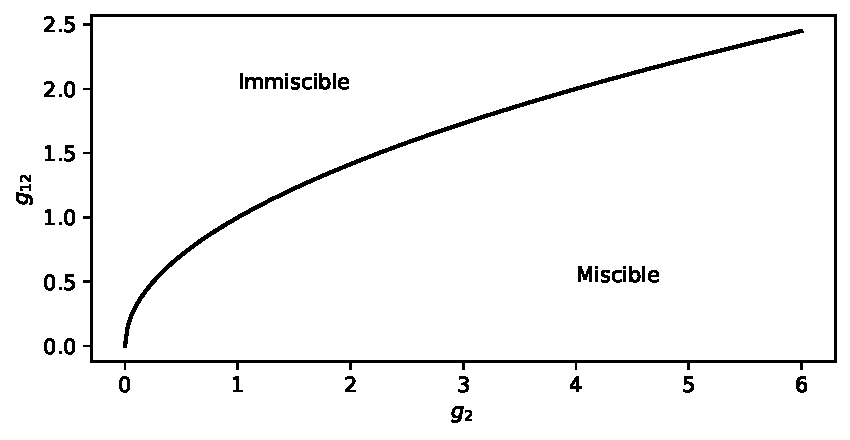
\includegraphics{gfx/ch-theory/miscible_vs_immiscible.pdf}
    \caption[Two-component miscible vs immiscible boundary]
    {\label{fig: miscible-vs-immiscible}Boundary between the miscible
        and immiscible regimes for a two-component condensate with \(g_1=1\).}
\end{figure}


\section{Spinor Bose-Einstein condensates}
Spinor systems comprise particles with total spin \(f\).
This implies there are \(2f + 1\) possible spin states along a given spin
quantisation axis.
Such a state is denoted \(\ket{f, m} \), where
\(m \in \{-f, -f+1, \ldots, 0, \ldots, f - 1, f\} \) denotes the magnetic
sublevel for total spin \( f\).

A general spin-\(f\) state is described by the (\(2f+1\))-component wave
function \(\psi \), defined as \(\ket{\psi} = \sum_m\psi_m\ket{f, m}\).
In the spin-1 case, we have \(\psi = {(\psi_1, \psi_0, \psi_{-1})}^T\), and for
the spin-2 case \(\psi = {(\psi_2, \psi_1, \psi_0, \psi_{-1}, \psi_{-2})}^T\).

Two identical spin-\(f\) bosons (atoms with integer spin) can collide to form a
total spin of \(\EuScript{F} = 0, 2, \ldots, 2f\) depending on the orientation
of the particles, with \(\EuScript{M} \equiv m+m' \in
\{-\EuScript{F}, \ldots, \EuScript{F}\} \).
In the s-wave scattering limit, where the orbital angular momentum is zero,
the total spin of two interacting particles must be even.
Due to the rotational symmetry, the scattering lengths depend only on the total
spin \(\EuScript{F}\), implying there are \(f + 1\) different scattering lengths
\(a_0, a_2, \ldots, a_{2f}\).

In a spinor BEC, the effective contact interaction is generalised to include
contributions from all spin channels as
\begin{equation}\label{eq: spin-f-interaction-potential}
    V_\mathrm{int} = \delta(\vb{r_1} - \vb{r_2})
    \sum_{\EuScript{F}=0}^{2f}g_\EuScript{F}\vb{P}_\EuScript{F},
\end{equation}
where \(g_\EuScript{F}=4\pi\hbar^2a_\EuScript{F}/M\) and
\(\vb{P}_\EuScript{F}\) is the projection operator which projects a pair
of atoms into a total spin \(\EuScript{F}\) state, defined as
\begin{equation}
    \vb{P}_\EuScript{F} = \sum_{m=-\EuScript{F}}^{\EuScript{F}}
    \ket{\EuScript{F}, \EuScript{M}}\bra{\EuScript{F}, \EuScript{M}}.
\end{equation}
For a system of identical bosons, the sum over all projection operators gives
\begin{equation}\label{eq: completeness-relation}
    \sum_{\EuScript{F}=0}^{2f}\vb{P}_\EuScript{F} = 1.
\end{equation}


\subsection{Spin-1 interaction Hamiltonian}\label{subsec: spin-1-int-hamil}
To calculate the spin-dependent mean-field interaction potential, it is common
to relate the projection operators to products of the single-particle spin
operators.
For a spin-1 condensate, the composition law of the angular momentum
gives~\cite{Kawaguchi2012, StamperKurn2013}
\begin{equation}\label{eq: composition-law}
    \vb{F}_1 \cdot \vb{F}_2 = \frac{1}{2}\left[{(\vb{F}_1 + \vb{F}_2)}^2
        - \vb{F}_1^2 - \vb{F}_2^2\right] = \frac{1}{2}\EuScript{F}(\EuScript{F} + 1)
    -f(f+1),
\end{equation}
where \(\vb{F}_i\) is the spin operator for atom \(i\).
From here we can construct the relation \(\vb{F}_1 \cdot \vb{F}_2 =
\sum_{\EuScript{F} = 0}^{2f}\lambda_\EuScript{F}\vb{P}_\EuScript{F}\), where
\(\lambda_\EuScript{F} = \frac{1}{2}\EuScript{F}(\EuScript{F} + 1)
-f(f+1)\).
In an \(f=1\) spinor condensate, only \(\EuScript{F} = 0\) or \(2\) channels
are allowed.
Therefore, we have
\begin{equation}\label{eq: spin-1-spin-relation}
    \vb{F}_1 \cdot \vb{F}_2 = \sum_{\EuScript{F} = 0}^{2f}
    \lambda_\EuScript{F}\vb{P}_\EuScript{F} = \vb{P}_2 - 2\vb{P}_0,
\end{equation}
and
\begin{equation}\label{eq: spin-1-completeness-relation}
    \sum_{\EuScript{F} = 0}^{2f} = 1 = \vb{P}_0 + \vb{P}_2.
\end{equation}
Using both Eq.~\eqref{eq: spin-1-spin-relation} and
Eq.~\eqref{eq: spin-1-completeness-relation}, one can re-write
Eq.~\eqref{eq: spin-f-interaction-potential} as
\begin{equation}
    V_\mathrm{int} = \delta(\vb{r}_1 - \vb{r}_2)
    (c_0 + c_1 \vb{F}_1 \cdot \vb{F}_2),
\end{equation}
where \(c_0 = (g_0+2g_2)/3\) and \(c_1=(g_2-g_0) / 3\).
Finally, the spin-1 interacting Hamiltonian is then given as
\begin{equation}\label{eq: spin-1-interacting-Hamiltonian}
    H_\mathrm{int} = \frac{1}{2}\int d\vb{r} (c_0n^2 + c_1|\vb{F}|^2).
\end{equation}

Here \(c_0\) is interpreted as the spin-independent interaction strength.
It becomes apparent from Eq.~\ref{eq: spin-1-interacting-Hamiltonian} that
\(c_0 > 0\) (repulsive interactions) is required for stability.
In the \(c_0 < 0\) limit (i.e., attractive interactions), the condensate would
favour becoming infinitely dense, and in the process would destroy itself.
Therefore, throughout this thesis we always consider \(c_0 > 0\).

The \(c_1\) term describes is the spin-dependent interaction strength.
Since \(c_0\) is constrained to be positive, \(c_1\) can take positive or
negative values.
When \(c_1 > 0\), the system energetically favours minimising the condensate
spin \(\vb{F}\), which are typically referred to as antiferromagnetic or polar
interactions.
Conversely, for \(c_1 < 0\) the system favours maximising the spin vector,
which are referred to as ferromagnetic interactions.

Finally, we note that since \(c_1\) is the difference of two s-wave scattering
lengths which are comparable in magnitude experimentally, the spin-dependent
interaction strength is usually much smaller than the spin-independent strength.

\subsection{Spin-2 interaction Hamiltonian}
For an \(f=2\) spinor condensate, we now have \(\EuScript{F}=0,2,4\) spin
channels.
For a spin-2 condensate, Eq.~\eqref{eq: composition-law} now gives
\begin{equation}
    \vb{F}_1 \cdot \vb{F}_2 = \sum_{\EuScript{F} = 0}^{2f}
    \lambda_\EuScript{F}\vb{P}_\EuScript{F} = -6\vb{P}_0-3\vb{P}_2+4\vb{P}_4.
\end{equation}
Using the above equation and the completeness relation in
Eq.~\eqref{eq: completeness-relation}, one can write \(\vb{P}_2\) and
\(\vb{P}_4\) in terms of \(\vb{P}_0\) and \(\vb{F}_1 \cdot \vb{F}_2\):
\begin{equation}
    \vb{P}_2 = \frac{1}{7}(4 - \vb{F}_1 \cdot \vb{F}_2 - 10\vb{P}_0), \qquad
    \vb{P}_4 = \frac{1}{7}(3 + \vb{F}_1 \cdot \vb{F}_2 + 3\vb{P}_0).
\end{equation}
From Eq.~\eqref{eq: spin-f-interaction-potential}, the spin-2 interaction
potential takes the form
\begin{equation}
    V_\mathrm{int}\delta(\vb{r}_1-\vb{r}_2)(c_0+c_1\vb{F}_1 \cdot \vb{F}_2
    +c_2\vb{P}_0),
\end{equation}
where \(c_0=(4g_2+3g_4)/7\), \(c_1=(g_4-g_2)/7\), and
\(c_2=(7g_0-10g_2+3g_4)/7\).
Both \(c_0\) and \(c_1\) are the spin-independent and -dependent interaction
strengths, respectively, analogous to the spin-1 system.
Due to the extra degree of freedom in the spin-2 system, a new interaction term,
\(c_2\), describing the spin-singlet interaction arises.

The spin-2 interaction Hamiltonian is given as
\begin{equation}\label{eq: spin-2-interacting-Hamiltonian}
    H_\mathrm{int} = \frac{1}{2}\int d\vb{r}\left(c_0n^2+c_1|\vb{F}|^2
    +c_2|A_{20}|^2\right),
\end{equation}
where \(|A_{20}|^2\) is the spin-singlet duo amplitude, defined in terms of
the condensate wave function as
\begin{equation}\label{eq: spin-singlet-duo}
    A_{20} = \frac{1}{\sqrt{5}}\left(\psi_0^2-2\psi_1\psi_{-1}
    +2\psi_2\psi_{-2}\right).
\end{equation}
For \(c_2 > 0\), it becomes energetically favourable to minimise the
spin-singlet amplitude, i.e., \(|A_{20}|^2 = 0\).
Conversely, for interactions where \(c_2 < 0\), the energy is minimised by
maximising the amplitude \(|A_{20}|^2=n/5\).

\subsection{Single-particle Hamiltonian}
When a magnetic field is applied to a spinor system, the field causes energy
shifts in the spin components.
When this field is aligned along the spin quantisation axis, linear, \(p\), and
quadratic, \(q\), Zeeman shifts arise.
In such a case, the single-particle (non-interacting) Hamiltonian is given
by~\cite{Kawaguchi2012}
\begin{equation}\label{eq: single-particle-Hamiltonian}
    H_0 = \int d\vb{r}\sum_{m,m'=-f}^{f} \psi_m^\dagger \left[
        -\frac{\hbar^2}{2M}\nabla^2 + V(\vb{r}) - pm + qm^2\right]\psi_{m'},
\end{equation}
where \(V(\vb{r})\) is a trapping potential.
Throughout most of this thesis we assume that the magnetic field applied is
uniform, such that the Zeeman shifts are constant.
In Chapter~\ref{chap: spin-1}, however, we introduce a time-dependent field
such that the quadratic Zeeman shift has a time-dependence.
Despite the time-dependence, the quadratic Zeeman shift is still spatially
uniform.

It becomes apparent from Eq.~\eqref{eq: single-particle-Hamiltonian} that the
quadratic shift uniformly alters the energetic separation between the
\(\psi_{\pm 1}\) and \(\psi_0\) components.
Conversely, the linear shift maintains the separation.

\section{Spinor Gross-Pitaevskii equations}
\subsection{Spin-1}\label{subsec: spin-1-gpes}
Combing the results of the previous sections, the energy functional of a spin-1
BEC is given as~\cite{Kawaguchi2012}
\begin{equation}\label{eq: spin-1-energy-functional}
    E = \int \left[\sum_{m=-1}^1\psi_m^*\left(-\frac{\hbar^2\nabla^2}{2M}
        + V(\vb{r}) - pm + qm^2\right)\psi_m + \frac{c_0}{2}n^2
        + \frac{c_1}{2}|\vb{F}|^2\right] d^3\vb{r},
\end{equation}
where \(n(\vb{r}) = \sum_{m=-1}^{1}|\psi_m(\vb{r})|^2\) is the total particle
density of the system.
Here, \(\vb{F}=(F_x, F_y, F_z)\) is the spin density vector, defined as
\begin{equation}\label{eq: spinor-spin-vector}
    F_\nu(\vb{r}) = \sum_{m,m'=-1}^{1}\psi_m^*(\vb{r}){(\vb{f}_\nu)}_{mm'}
    \psi_{m'}(\vb{r}), \qquad (\nu=x, y, z).
\end{equation}
The spin-1 Pauli matrices \(\vb{f}_\mu \) are given in the irreducible
representation as
\begin{equation}\label{eq: spin-1-Pauli-matrices}
    \vb{f}_x = \frac{1}{\sqrt{2}}\mqty(0 & 1 & 0 \\ 1 & 0 & 1 \\ 0 & 1 & 0),
    \qquad
    \vb{f}_y = \frac{i}{\sqrt{2}}\mqty(0 & -1 & 0 \\ 1 & 0 & -1 \\ 0 & 1 & 0),
    \qquad
    \vb{f}_z = \mqty(1 & 0 & 0 \\ 0 & 0 & 0 \\ 0 & 0 & -1).
\end{equation}
Substituting Eq.~\eqref{eq: spin-1-Pauli-matrices} into
Eq.~\eqref{eq: spinor-spin-vector} gives the exact expressions of the spin-1
spin vectors:
\begin{align}\label{eq: spin-1-spin-vectors}
    F_x & = \frac{1}{\sqrt{2}} \left(\psi_1^*\psi_0 + \psi_0^*(\psi_1+\psi_{-1})
    + \psi_{-1}^*\psi_0\right)                                                   \\
    F_y & = \frac{i}{\sqrt{2}}\left(-\psi_1^*\psi_0 + \psi_0^*(\psi_1-\psi_{-1})
    +\psi_{-1}^*\psi_0\right)                                                    \\
    F_z & = |\psi_1|^2-|\psi_{-1}|^2.
\end{align}

The spin-1 Gross-Pitaevskii equations are derived, though lengthy, from the
variational derivative of the energy functional in
Eq.~\eqref{eq: spin-1-energy-functional} as \(i\hbar\delta E/\delta \psi_m^*\).
This results in
\begin{equation}\label{eq: spin-1-GPEs}
    i\hbar \pdv{\psi_m}{t} = \left[-\frac{\hbar^2\nabla^2}{2M} + V(\vb{r})
        - pm + qm^2 + c_0n\right]\psi_m
    + c_1\sum_{m'=-1}^{1}\vb{F}\cdot \vb{f}_{mm'}\psi_{m'},
\end{equation}
which describe the mean-field evolution of spin-1 Bose-Einstein condensates.

Time-independent equations are found through the substitution
\(\psi_m = \psi_m(\vb{r})e^{-i\mu t/\hbar}\), where \(\mu \) is the chemical
potential.
Substituting into Eq.~\eqref{eq: spin-1-GPEs} and writing the equation for
each component explicitly gives
\begin{align}\label{eq: spin-1-GPEs-dimensional-psi1}
    \left[-\frac{\hbar^2\nabla^2}{2M} + V(\vb{r}) - p + q + c_0n + c_1F_z
    - \mu\right]\psi_1 + \frac{c_1}{\sqrt{2}}F_-\psi_0    & = 0  \\
    \frac{c_1}{\sqrt{2}}F_+\psi_1 + \left[-\frac{\hbar^2\nabla^2}{2M}
        + V(\vb{r}) + c_0n - \mu\right]\psi_0 + \frac{c_1}{\sqrt{2}}F_-\psi_{-1}
                                                          & = 0  \\
    \left[-\frac{\hbar^2\nabla^2}{2M} + V(\vb{r}) + p + q + c_0n - c_1F_z
    - \mu\right]\psi_{-1} + \frac{c_1}{\sqrt{2}}F_+\psi_0 & = 0,
    \label{eq: spin-1-GPEs-dimensional-psim1}
\end{align}
where \(F_{\pm} = F_x \pm iF_y\).
These equations can be solved to reveal more on the ground states and stationary
solutions of spinor BECs, which forms the basis of
Chapter~\ref{chap: ground-states}.

\subsection{Spin-2}
The spin-2 energy functional is written as~\cite{Kawaguchi2012}
\begin{equation}\label{eq: spin-2-energy-functional}
    E = \int \left[\sum_{m=-2}^{2}\psi_m^* \left(-\frac{\hbar^2\nabla^2}{2M}
    + V(\vb{r}) -pm + qm^2\right)\psi_m + \frac{c_0}{2}n^2
    + \frac{c_1}{2}|\vb{F}|^2 + \frac{c_2}{2}|A_{20}|^2\right] d^3\vb{r}.
\end{equation}
The spin-2 Pauli matrices are given in irreducible representation as
\begin{equation*}
    \vb{f}_x = \mqty(0 & 1  & 0 & 0 & 0 \\
    1 & 0 & \sqrt{\frac{3}{2}} & 0 & 0 \\
    0 & \sqrt{\frac{3}{2}} & 0 & \sqrt{\frac{3}{2}} & 0 \\
    0 & 0 & \sqrt{\frac{3}{2}} & 0 & 1 \\
    0 & 0 & 0 & 1 & 0), \qquad
    \vb{f}_y = \mqty(0 & -i  & 0 & 0 & 0 \\
    i & 0 & -i\sqrt{\frac{3}{2}} & 0 & 0 \\
    0 & i\sqrt{\frac{3}{2}} & 0 & -i\sqrt{\frac{3}{2}} & 0 \\
    0 & 0 & i\sqrt{\frac{3}{2}} & 0 & -i \\
    0 & 0 & 0 & i & 0),
\end{equation*}
\begin{equation}
    \vb{f}_z = \mqty(2 & 0 & 0 & 0 & 0 \\
    0 & 1 & 0 & 0 & 0 \\
    0 & 0 & 0 & 0 & 0 \\
    0 & 0 & 0 & -1 & 0 \\
    0 & 0 & 0 & 0 & -2).
\end{equation}

Similar to the spin-1 case, the GPEs are obtained through the variational
derivative of Eq.~\eqref{eq: spin-2-energy-functional}, resulting in
five coupled equations that model the mean-field dynamics of spin-2
Bose-Einstein condensates.
\begin{align}
    i\hbar\pdv{\psi_{\pm 2}}{t} & = \left[-\frac{\hbar^2\nabla^2}{2M}
        + V(\vb{r}) \mp 2p + 4q + c_0n \pm 2c_1F_z - \mu\right]\psi_{\pm 2}
    + c_1F_{\mp}\psi_{\pm 1} + \frac{c_2}{\sqrt{2}}A_{20}\psi_{\mp 2}^*
    \label{eq: spin-2-GPEs-pm2}                                            \\
    i\hbar\pdv{\psi_{\pm 1}}{t} & = \left[-\frac{\hbar^2\nabla^2}{2M}
        + V(\vb{r}) \mp p + q + c_0n \pm c_1F_z - \mu\right]\psi_{\pm 1}
    + c_1\left(\frac{\sqrt{6}}{2}F_{\mp}\psi_0 + F_{\pm}\psi_{\pm 2}\right)
    - \frac{c_2}{\sqrt{2}}A_{20}\psi_{\mp 1}^* \label{eq: spin-2-GPEs-pm1} \\
    i\hbar\pdv{\psi_0}{t}       & = \left[-\frac{\hbar^2\nabla^2}{2M}
        + V(\vb{r}) + c_0n - \mu\right]\psi_0
    + \frac{\sqrt{6}}{2}c_1\left(F_+\psi_1 + F_-\psi_{-1}\right)
    + \frac{c_2}{\sqrt{2}}A_{20}\psi_{\mp 2}^*, \label{eq: spin-2-GPEs-0}
\end{align}
where the spin vectors are given as
\begin{align}\label{eq: spin-2-spin-vectors}
    F_+ = F_-^* & = 2(\psi_2^*\psi_1 + \psi_{-1}^*\psi_{-2})
    + \sqrt{6}(\psi_1^*\psi_0 + \psi_0^*\psi_{-1}),                             \\
    F_z         & = 2(|\psi_2|^2 - |\psi_{-2}|^2) + |\psi_1|^2 - |\psi_{-1}|^2.
\end{align}

Following the same procedure as in the spin-1 case, the time-independent GPEs
can be found through the substitution
\(\psi_m(\vb{r}, t) = \psi_m(\vb{r})e^{-\mu t/\hbar}\).
\textcolor{red}{Worth listing time-independent GPEs for spin-2 case?}

\subsection{Conserved quantities}
In spinor BECs, there are three conserved quantities.
Firstly, the total energy of the system
    [Eq.~\eqref{eq: spin-1-energy-functional} and
        Eq.~\eqref{eq: spin-2-energy-functional}] is conserved.
In addition, the total atom number of the condensate
\begin{align}
    N = \int \sum_m |\psi_m|^2 d^3\vb{r}
\end{align}
is also conserved.
Different from the scalar case, however, is the additional conservation of the
\(z\)-component of the magnetisation
\begin{align}\label{eq: magnetisation-formula}
    M_z = \int F_z d^3\vb{r},
\end{align}
where \(F_z\) is given in Eq.~\eqref{eq: spin-1-spin-vectors} or
Eq.~\eqref{eq: spin-2-spin-vectors} for the spin-1 and spin-2 cases,
respectively.
\textcolor{red}{Appendix on derivations?}

\section{Reduction to lower dimensions}
One can reduce the full 3D coupled GPEs to lower dimensions by considering
sufficiently tight confinement of the condensate in one or more directions.
Here, we reduce both the spin-1 and spin-2 GPEs to their 2D and 1D counterparts.

\subsection{Spin-1}
To begin, we start with the full 3D dimensional equations given in
Eqs.~\eqref{eq: spin-1-GPEs-dimensional-psi1} ---
~\eqref{eq: spin-1-GPEs-dimensional-psim1}, written in matrix form as
\begin{align}\label{eq: spin-1-GPEs-matrix}
    i\hbar \pdv{\Psi}{t} = \left[-\frac{\hbar^2\nabla^2}{2M} + V(\vb{r}) + c_0n
    + c_1n \langle\hat{\vb{F}}\rangle \cdot \hat{\vb{F}} - p\hat{F}_z
    + q\hat{F}_z^2\right]\Psi,
\end{align}
where \(\Psi=(\psi_1, \psi_0, \psi_{-1})\) is the three-component wave function.
\textcolor{red}{Has \(\hat{\vb{F}}\) been defined before?}
To reduce the dimensionality, we assume the condensate has been tightly confined
in the \(z\) direction by means of a harmonic oscillator which has trapping
frequencies (\(\omega_x, \omega_y, \omega_z\)) in the (\(x, y, z\)) directions,
respectively.
A tight confinement in the \(z\) direction is achieving by having
\(\omega_z \gg \omega_x, \omega_y\).
In addition, we assume the trapping frequencies are sufficiently such that only
the ground state of the condensate is occupied.
With these assumptions, we can separate the wave function of the condensate into
its 2D counterpart:
\begin{align}\label{eq: Psi-2D}
    \Psi(x, y, z, t) = \tilde{\Psi}(x, y, t)\Phi(z)
    = \sqrt{\tilde{n}(x, y, t)}\zeta(x, y, t)\Phi(z),
\end{align}
where \(\Phi(z)\) is normalised as \(\int_{-\infty}^{\infty}|\Phi(z)|^2 \, \dd z
= 1\), and we apply the single-mode approximation (SMA) such that
\(\zeta(x, y, t)\) has no \(z\)-dependence.

Substituting Eq.~\eqref{eq: Psi-2D} into Eq.~\eqref{eq: spin-1-GPEs-matrix} we
obtain
\begin{equation}
\begin{split}
    i\hbar\pdv{\tilde{\Psi}}{t}\Phi = \left[
        -\frac{\hbar^2}{2M}\Phi\nabla_\perp^2
        - \frac{\hbar^2}{2M}\pdv[2]{\Phi}{z} + [V_\perp(x, y) + V_z(z)]\Phi
        +c_0\tilde{\Psi}^\dagger\tilde{\Psi}|\Phi|^2\Phi\right. \\
        \left.+c_1\tilde{\Psi}^\dagger\tilde{\Psi}|\Phi|^2\Phi
        \langle\hat{\vb{F}}\rangle \cdot \hat{\vb{F}}
        -p\Phi\hat{F}_z + q\Phi\hat{F}_z^2 \vphantom{\int_1^2}\right]\Psi.
\end{split}
\end{equation}
To reduce the equation further, we multiply from the left by \(\Phi^*\) and
integrate over the \(z\) direction, which gives:
\begin{equation}\label{eq: spin-1-GPEs-tildes}
\begin{split}
    \left[
        -\frac{\hbar^2}{2M}\Phi\nabla_\perp^2
        - \frac{\hbar^2}{2M}\int_{-\infty}^{\infty}\Phi^*\dv[2]{\Phi}{z} \dd z
        + V_\perp(x, y) + \int_{-\infty}^{\infty} V_z(z)|\Phi|^2 \dd z\right. \\
        \left.+c_0\tilde{n}\int_{-\infty}^{\infty}|\Phi|^4 \dd z
        +c_1\tilde{n}\langle\hat{\vb{F}}\rangle \cdot \hat{\vb{F}}
        \int_{-\infty}^{\infty}|\Phi|^4 \dd z
        -p\hat{F}_z + q\Phi\hat{F}_z^2 \right]\Psi.
\end{split}
\end{equation}
In the above equation, the constant \(C =
-\frac{\hbar^2}{2M}\int_{-\infty}^{\infty}\Phi^*\dv[2]{\Phi}{z} \dd z
+ \int_{-\infty}^{\infty} V_z(z)|\Phi|^2 \dd z\) can be removed from the
equation via the appropriate transformation \(\tilde{\Psi} \rightarrow
\tilde{\Psi}e^{-Ct/N}\), where \(N\) is the total atom number.
Now, we take \(\Phi(z)\) to be the harmonic oscillator ground state, which has
the form
\begin{align}
    \Phi(z) =
    {\left(\frac{\beta}{\pi}\right)}^{\frac{1}{4}}e^{-\frac{\beta}{2}z^2},
\end{align}
where \(\beta = M\omega_z/\hbar \).
This then leads to the integral
\begin{align}
    \int_{-\infty}^{\infty}|\Phi(z)|^4 \dd z = \sqrt{\frac{\beta}{2\pi}}.
\end{align}
We can then appropriately rescale the interaction strengths into their 2D
counterparts:
\begin{align}
    c_0^\text{2D} = c_0\sqrt{\frac{\beta}{2\pi}}, \qquad
    c_1^\text{2D} = c_1\sqrt{\frac{\beta}{2\pi}}.
\end{align}
Finally, substituting back into Eq.~\eqref{eq: spin-1-GPEs-tildes} yields the
2D GPEs for a spin-1 system:
\begin{align}
    i\hbar\pdv{\Psi}{t} = \left[-\frac{\hbar^2}{2M}\nabla_\perp^2 + V_\perp
    + c_0^\text{2D}n + c_1^\text{2D}n\langle\hat{\vb{F}}\rangle \cdot \hat{\vb{F}}
    -p\hat{F}_z + q\hat{F}_z^2\right]\Psi,
\end{align}
where we have dropped the tildes for notational convenience.

A similar process can be used to reduce the full 3D equations into their 1D
counterparts.
We now assume that the condensate is tightly confined in two directions, which
we will take to be the \(x, y\) directions (\(\omega_x, \omega_y \gg
\omega_z\)).
This time, we separate the wave function according to
\begin{align}
    \Psi(x, y, z, t) = \tilde{\Psi}(z, t)\Phi(x, y) = \sqrt{\tilde{n}(z, t)}
    \zeta(z, t)\Phi(x, y),
\end{align}
once again assuming \(\Phi(x, y)\) to be normalised as \(\int_{-\infty}^{\infty}
\int_{-\infty}^{\infty} |\Phi(x, y)|^2 \dd x \dd y = 1\) and using the SMA such
that \(\zeta(z, t)\) only has a \(z\) dependence.
We substitute the above expression in the GPEs
(Eq.~\eqref{eq: spin-1-GPEs-matrix}) and find
\begin{equation}
\begin{split}
    i\hbar\pdv{\tilde{\Psi}}{t}\Phi = \left[
        -\frac{\hbar^2}{2M}\Phi\pdv[2]{}{z}
        - \frac{\hbar^2}{2M}\nabla_\perp^2\Phi + [V_\perp(x, y) + V_z(z)]\Phi
        +c_0\tilde{\Psi}^\dagger\tilde{\Psi}|\Phi|^2\Phi\right. \\
        \left.+c_1\tilde{\Psi}^\dagger\tilde{\Psi}|\Phi|^2\Phi
        \langle\hat{\vb{F}}\rangle \cdot \hat{\vb{F}}
        -p\Phi\hat{F}_z + q\Phi\hat{F}_z^2 \vphantom{\int_1^2}\right]\Psi.
\end{split}
\end{equation}
Following the procedure before, we multiply from the left by \(\Phi^*\)
and integrate over \(x\) and \(y\) which yields
\begin{equation}
\begin{split}
    \left[
        -\frac{\hbar^2}{2M}\Phi\pdv[2]{}{z}
        - \frac{\hbar^2}{2M}\int_{-\infty}^{\infty}\int_{-\infty}^{\infty}
        \Phi^*\dv[2]{\Phi}{z} \dd x \dd y
        + V_\perp(x, y) + \int_{-\infty}^{\infty}\int_{-\infty}^{\infty}
        V_z(z)|\Phi|^2 \dd x \dd y\right. \\
        \left.+c_0\tilde{n}\int_{-\infty}^{\infty}\int_{-\infty}^{\infty}
        |\Phi|^4 \dd x \dd y
        +c_1\tilde{n}\langle\hat{\vb{F}}\rangle \cdot \hat{\vb{F}}
        \int_{-\infty}^{\infty}\int_{-\infty}^{\infty}|\Phi|^4 \dd x \dd y
        -p\hat{F}_z + q\Phi\hat{F}_z^2 \right]\Psi.
\end{split}
\end{equation}
Now, the constant term \(C = -\hbar^2/2M\int_{\infty}^{\infty}
\int_{\infty}^{\infty}|\nabla_\perp^2\Phi|^2\dd x \dd z
+\int_{\infty}^{\infty}\int_{\infty}^{\infty}V_\perp|\Phi|^2\dd x \dd y\) can
again be dropped from the equation via the appropriate substitution
\(\tilde{\Psi} = \tilde{\Psi}e^{-iCt/N}\).
We then take \(\tilde{\Psi}\) to be the lowest harmonic oscillator ground state,
which in 2D becomes
\begin{align}
    \Phi(x, y) = {\left(\frac{\beta}{\pi}\right)}^{1/2}
    e^{-\frac{\beta}{2}(x^2+y^2)},
\end{align}
where \(\beta=m\omega_\perp / \hbar \), which leads to the relation
\begin{align}
    \int_{\infty}^{\infty}\int_{\infty}^{\infty} |\Phi(x, y)|^4 \dd x \dd y
    = \frac{\beta}{2\pi}.
\end{align}
This then leads to the 1D rescaled interaction strengths
\begin{align}
    c_0^\text{1D} = c_0\frac{\beta}{2\pi}, \qquad
    c_1^\text{1D}=c_1\frac{\beta}{2\pi}.
\end{align}
Finally, we arrive at the 1D GPE given in matrix form:
\begin{align}
    i\hbar\pdv{\Psi}{t} = \left[-\frac{\hbar^2}{2M}
    \pdv[2]{}{z}+V_z(z) + c_0^\text{1D}n
    + c_1^\text{1D}\langle\hat{\vb{F}}\rangle \cdot \hat{\vb{F}} - p\hat{F}_z
    + q\hat{F}_z^2\right]\Psi,
\end{align}
again dropping the tildes for notational convenience.

\section{Dimensionless spinor Gross-Pitaevskii equations}
\label{sec: dimensionless-equations}
Systems that can undergo Bose-Einstein condensation, and hence become a
superfluid, can form at a variety of length scales, ranging from Bose-Einstein
condensates at the micron scale all the way to the cores of neutron stars,
which are theorised to be superfluid on the kilometre
scale~\cite{Warszawski2011}.
In addition, atomic Bose-Einstein condensates in experiment take on a wide range
of variable parameters and geometries.
Such geometries include box-like potentials~\cite{Gaunt2013}, toroidal ring
geometries~\cite{Ryu2007, Ramanathan2011}, both quasi-2D~\cite{Neely2010}
and quasi-1D systems~\cite{Burger1999}, and even arbitrary
potentials~\cite{Henderson2009}.

Due to these reasons, rescaling the quantities used in the corresponding GPEs
allows one to reformulate any calculation into a desired scale and parameter
regime.
In practice, this is done by casting the GPEs into a dimensionless form, where
each dimensional parameter in the equation is rescaled using an appropriate
quantity such that it becomes dimensionless.
An advantage of using a dimensionless form is that the parameters used within
numerical computation become normalised on the scale of unity, which,
when compared to values in the dimensional equation such as \(\hbar =
1.054\times 10^{-34}\), can reduce numerical errors that arise due to the
floating point representation used by computers.

The process of making the GPEs dimensionless can be done in different ways,
where the scaling parameters chosen typically depend on whether the system is
trapped or not.
Here, we derive the dimensionless 3D GPEs for both a homogeneous spin-1 BEC and
a trapped spin-2 BEC, which will aid the analysis in subsequent chapters.

\subsection{Homogeneous spin-1 BEC}
Consider a homogeneous system in the absence of a trapping potential
\(V(\vb{r}) = 0\).
In a spin-1 system, there are two choices of length scales one
can choose as their unit of length: the density healing length
\(\xi_d=\hbar /\sqrt{2Mc_0n_0}\), or the spin healing length
\(\xi_s = \hbar /\sqrt{2M|c_1|n_0}\), where \(n_0\) is the background density
of the uniform system.
Both choices are valid, but for this thesis we shall choose the spin healing
length, \(\xi_s\).
Then, an appropriate unit of energy is the spin energy: \(E_s = 2|c_1|n_0\),
which leads to the spin time \(\tau_s = \hbar / E_s\).
Now we have found appropriate units for length, time, and energy, we can
rescale each quantity as
\begin{align}
    \vb{r} \rightarrow \xi_s \tilde{\vb{r}}, \qquad
    t \rightarrow \tau_s\tilde{t}, \qquad
    \Psi \rightarrow \sqrt{n_0}\tilde{\Psi},
\end{align}
where a tilde denotes the dimensionless quantity.
Substituting these into Eq.~\eqref{eq: spin-1-GPEs-matrix} leads to the
dimensionless spin-1 GPEs:
\begin{align}
    i \pdv{\tilde{\psi}_{1}}{\tilde{t}} &= \left[-\frac{1}{2}\tilde{\nabla}^2
    + \tilde{c}_0\tilde{n} + \tilde{c}_1\tilde{n}\tilde{F}_z - \tilde{p}
    + \tilde{q}\right]\tilde{\psi}_{1}
    + \frac{\tilde{c}_1}{\sqrt{2}}\tilde{F}_-\tilde{\psi}_0, \\
    i \pdv{\tilde{\psi}_0}{\tilde{t}} &= \left[-\frac{1}{2}\tilde{\nabla}^2
    + \tilde{c}_0\tilde{n}\right]\tilde{\psi}_0
    + \frac{\tilde{c}_1}{\sqrt{2}}\left(\tilde{F}_+\tilde{\psi}_1
    + \tilde{F}_-\tilde{\psi}_{-1}\right), \\
    i \pdv{\tilde{\psi}_{-1}}{\tilde{t}} &= \left[-\frac{1}{2}\tilde{\nabla}^2
    + \tilde{c}_0\tilde{n} - \tilde{c}_1\tilde{n}\tilde{F}_z + \tilde{p}
    + \tilde{q}\right]\tilde{\psi}_{-1}
    + \frac{\tilde{c}_1}{\sqrt{2}}\tilde{F}_+\tilde{\psi}_0, \\
\end{align}
where the rescaled interaction strengths and Zeeman shifts are
\begin{align}
    \tilde{c}_0 = \frac{n_0c_0}{E_s} = \left|\frac{c_0}{2c_1}\right|, \quad
    \tilde{c}_1 = \frac{n_0c_1}{E_s} = \frac{1}{2} \cdot \text{sgn}(c_1),\quad
    \tilde{p} = \frac{q}{E_s}, \quad
    \tilde{q} = \frac{q}{E_s}.
\end{align}
By choosing our unit of length and time as \(\xi_s\) and \(\tau_s\),
respectively, the dimensionless spin-dependent interaction strength is fixed
at \(|\tilde{c}_1| = 1/2\).
Therefore, to set the spin-independent interaction strength, \(\tilde{c}_0\),
we need the ratio of the interaction strengths, \(c_0/c_1\), which is set by
the atomic species itself.

\subsection{Trapped spin-2 BEC}\label{subsec: spin-2-dimensionless}
Consider now a spin-2 BEC trapped by a uniform harmonic trap \(V(\vb{r})\).
Now, instead of choosing the healing length as our unit of length, it makes more
sense to instead choose the harmonic oscillator length \(\ell =
\sqrt{\hbar/(M\omega)}\), where \(\omega \) is the trapping frequency.
Then, time is measured in units of \(omega^{-1}\) and energy in
\(\hbar\omega \), which leads to the rescaling of the following units:
\(\vb{r}\rightarrow \ell\tilde{\vb{r}},\ t \rightarrow \omega\tilde{t}\).
To construct the dimensionless wave function, it is conventional to define the
dimensionless wave function as being normalised to unit
\(\int_{-\infty}^\infty |\tilde{\Psi}|^2\dd^3\tilde{\vb{r}} = 1\).
Then, recalling that the dimensional wave function is normalised to the number
of atoms \(\int_{-\infty}^\infty |{\Psi}|^2\dd^3{\vb{r}} = N\), and that
\(\dd^3\vb{r} = \ell^3\dd^3\tilde{\vb{r}}\), it follows that the dimensional
wave function can be rescaled as
\begin{align}
    \Psi \rightarrow \sqrt{\frac{N}{\ell^3}}\tilde{\Psi}.
\end{align}
Substituting these rescaled quantities into Eqs.~\eqref{eq: spin-2-GPEs-pm2}
-~\eqref{eq: spin-2-GPEs-0} yields the dimensionless spin-2 GPEs for a trapped
system
\begin{align}
    i\pdv{\tilde{\psi}_{\pm 2}}{\tilde{t}} &= \left[-\frac{1}{2}\tilde{\nabla}^2
    +V(\tilde{\vb{r}}) \tilde{c}_0\tilde{n} \pm 2\tilde{c}_1\tilde{F}_z
    \mp 2\tilde{p} + 4\tilde{q}\right]\tilde{\psi}_{\pm 2}
    + \tilde{c}_1\tilde{F}_\mp\tilde{\psi}_{\pm 1}
    + \frac{\tilde{c}_2}{\sqrt{2}}\tilde{A}_{20}\tilde{\psi}_{\mp 2}^* \\
    i\pdv{\tilde{\psi}_{\pm 1}}{\tilde{t}} &= \left[-\frac{1}{2}\tilde{\nabla}^2
    +V(\tilde{\vb{r}}) \tilde{c}_0\tilde{n} \pm \tilde{c}_1\tilde{F}_z
    \mp 2\tilde{p} + 4\tilde{q}\right]\tilde{\psi}_{\pm 1}
    +\tilde{c}_1\left(\frac{\sqrt{6}}{2}\tilde{F}_\mp \tilde{\psi}_0
    +\tilde{F}_\pm\tilde{\psi}_{\pm 2}\right)
    - \frac{\tilde{c}_2}{\sqrt{2}}\tilde{A}_{20}\tilde{\psi}_{\mp 1}^* \\
    i\pdv{\tilde{\psi}_0}{\tilde{t}} &= \left[-\frac{1}{2}\tilde{\nabla}^2
    +V(\tilde{\vb{r}})+\tilde{c}_0\tilde{n}\right]\tilde{\psi}_0
    +\frac{\sqrt{6}}{2}\tilde{c}_1\left(\tilde{F}_+\tilde{\psi}_1
    +\tilde{F}_-\tilde{\psi}_{-1}\right)
    + \frac{\tilde{c}_2}{\sqrt{2}}\tilde{A}_{20}\tilde{\psi}_{\pm 2}^*,
\end{align}
where now the rescaled interaction strengths and Zeeman shifts are
\begin{align}\label{eq: spin-2-interaction-strengths-dimensionless}
    \tilde{c}_0 = \frac{Nc_0}{\hbar\omega\ell^3}, \quad
    \tilde{c}_1 = \frac{Nc_1}{\hbar\omega\ell^3}, \quad
    \tilde{c}_2 = \frac{Nc_2}{\hbar\omega\ell^3}, \quad
    \tilde{p} = \frac{p}{\hbar\omega}, \quad
    \tilde{q} = \frac{q}{\hbar\omega}.
\end{align}

\subsection{Mapping to experimental parameters}
Numerical simulations are an extremely useful tool for gaining insight into
what experiments of BEC systems might look like.
Therefore, it is useful to calculate the values of the interaction strengths
for different atomic species so that they can be mapped to our dimensionless
parameters.
In particular, we investigate both the spin-1 and spin-2 atoms of \( ^{23}\)Na
and \( ^{87}\)Rb.
Here, we are taking our unit of length and time to be the harmonic oscillator
length \(\ell \) and inverse trap frequency \(\omega^{-1}\), respectively.

\subsubsection{Spin-1}
Recall that the dimensional interaction strengths for a spin-1 system are given
as
\begin{align}\label{eq: spin-1-interaction-strengths}
    c_0 = \frac{4\pi\hbar^2}{3M}(a_0+2a_2), \qquad
    c_1 = \frac{4\pi\hbar^2}{3M}(a_2-a_0), \qquad
\end{align}
where \(a_\mathcal{F}\) is the s-wave scattering length for the
spin-\(\mathcal{F}\) channel.
To calculate the dimensional interaction strengths, we list the scattering
lengths obtained by Crubellier~\cite{Crubellier1999} for \( ^{23}\)Na and
Ho~\cite{Ho1998} for \( ^{87}\)Rb in
Table~\ref{table: scaterring-lengths-spin-1}.
\begin{table}[htbp]
    \centering
    \begin{tabular}{ cccc } 
     \toprule
      & \(a_0\) & \(a_2\) \\
      \midrule
      \( ^{23}\)Na & \(50.0\pm 1.6\) & \(55.0\pm 1.7\) \\ 
      \( ^{87}\)Rb & \(110.0\pm 4.0\) & \(107.0\pm 4.0\) \\
      \bottomrule
    \end{tabular}
    \caption[Scattering lengths for spin-1 atomic species \( ^{23}\)Na and
    \( ^{87}\)Rb]{\label{table: scaterring-lengths-spin-1}Table of scattering
    lengths for spin-1 atomic species \( ^{23}\)Na and \( ^{87}\)Rb in units of
    the Bohr radius.}
\end{table}
With these values, we are free to calculate the dimensional interaction
strengths using Eq.~\eqref{eq: spin-1-interaction-strengths}.
To calculate the numerical, dimensionless interaction strengths we assume an
atom number of \(N = 2\times10^5\) and a trapping frequency of
\(\omega = 2\pi \times 130\)Hz.
Both the dimensional (with uncertainties) and dimensionless values for a spin-1
\( ^{23}\)Na system are given in Table~\ref{table: spin-1-interactions-sodium}.
\begin{table}[!htbp]
    \centering
    \begin{tabular}{ccc}
        \toprule
        \( ^{23}\)Na & Dimensional (units of \(\text{kg}\, \text{m}^5
        \text{s}^{-2}\)) & Dimensionless \\
        \midrule
        \(c_0\) & \(1.03 \pm 0.00321 \times 10^{-50}\) & \(3.91\times10^3\) \\
        \(c_1\) & \(3.21 \pm 0.0640 \times 10^{-52}\) & \(122\) \\
        \bottomrule
    \end{tabular}
    \caption{\label{table: spin-1-interactions-sodium}Dimensional (with
    uncertainties) and dimensionless interaction strengths of \( ^{23}\)Na.}
\end{table}
Calculating the ratio of interaction parameters gives \(c_0/c_1=32.0 \),
which predicts the ground state of \( ^{23}\)Na to be polar (see
Sec~\ref{sec: ground-states-spin-1} for details on spin-1 ground states).

For the \( ^{87}\)Rb system, we again assume an atom number of
\(N = 2\times 10^5\) with a trapping frequency of
\(\omega = 2\pi \times 130\)Hz.
The dimensional (with uncertainties) and dimensionless interaction strengths
for a spin-1 \( ^{87}\)Rb are given in
Table~\ref{table: spin-1-interactions-rb87}.
\begin{table}[!htbp]
    \centering
    \begin{tabular}{ccc}
        \toprule
        \( ^{87}\)Rb & Dimensional (units of \(\text{kg}\, \text{m}^5
        \text{s}^{-2}\)) & Dimensionless \\
        \midrule
        \(c_0\) & \(5.43 \pm 0.201 \times 10^{-51}\) & \(2.10\times10^3\) \\
        \(c_1\) & \(-5.03 \pm 10.3 \times 10^{-53}\) & \(-19.1\) \\
        \bottomrule
    \end{tabular}
    \caption{\label{table: spin-1-interactions-rb87}Dimensional (with
    uncertainties) and dimensionless interaction strengths of \( ^{23}\)Na.}
\end{table}
Calculating the ratio of interaction strengths for this system gives
\(c_0/c_1=-110 \), which predicts the ground state of \( ^{87}\)Rb to be
ferromagnetic (see
Sec~\ref{sec: ground-states-spin-1} for details on spin-1 ground states).

\subsubsection{Spin-2}\label{subsec: spin-2-experimental-parameters}
Recall that the dimensional interaction strengths for a spin-2 system are given
as
\begin{align}\label{eq: spin-2-interaction-strengths}
    c_0 = \frac{4\pi\hbar^2}{7M}(4a_2+3a_4), \qquad
    c_1 = \frac{4\pi\hbar^2}{7M}(a_4-a_2), \qquad
    c_2 = \frac{4\pi\hbar^2}{7M}(7a_0-10a_2+3a_4),
\end{align}
To determine the values of the interaction strengths, we first list the s-wave
scattering lengths in units of the Bohr radius given by
Ciobanu~\cite{Ciobanu2000} for \( ^{23}\)Na and Klausen~\cite{Klausen2001} for
\( ^{85}\)Rb and \( ^{87}\)Rb in Table~\ref{table: scaterring-lengths-spin-2}.
\begin{table}[htbp]
    \centering
    \begin{tabular}{ cccc } 
     \toprule
      & \(a_0\) & \(a_2\) & \(a_4\) \\
      \midrule
      \( ^{23}\)Na & \(34.9\pm 1.0\) & \(45.8\pm 1.1\) & \(64.5\pm 1.3\) \\ 
      \( ^{85}\)Rb  & \(-740\pm60.0\) & \(-570\pm 50.0\) & \(-390\pm20.0\) \\ 
      \( ^{87}\)Rb & \(86.2\pm 1.0\) & \(90.2\pm 1.0\) & \(97.4\pm 1.0\) \\
      \bottomrule
    \end{tabular}
    \caption[Table of scattering lengths for spin-2 atomic species \( ^{23}\)Na,
    \( ^{85}\)Rb, and \( ^{87}\)Rb]{\label{table: scaterring-lengths-spin-2}
    Table of scattering lengths for spin-2 atomic species \( ^{23}\)Na,
    \( ^{85}\)Rb, and \( ^{87}\)Rb in units of the Bohr radius.}
\end{table}
With these scattering lengths we can calculate the dimensional interaction
strengths using Eq.~\eqref{eq: spin-2-interaction-strengths}.
To calculate the corresponding dimensionless interaction strength, we assume
\(N = 2\times10^5\) and \(\omega = 2\pi \times 130\) Hz.
Both the dimensional (with uncertainties) and dimensionless values for a spin-2
\( ^{23}\)Na system are given in
Table~\ref{table: spin-2-interactions-sodium}.
\begin{table}[!htbp]
    \centering
    \begin{tabular}{ccc}
        \toprule
        \( ^{23}\)Na & Dimensional (units of \(\text{kg}\, \text{m}^5
        \text{s}^{-2}\)) & Dimensionless \\
        \midrule
        \(c_0\) & \(1.03 \pm 0.00654 \times 10^{-50}\) & \(3.91\times10^3\) \\
        \(c_1\) & \(5.10 \pm 0.654 \times 10^{-52}\) & \(195\) \\
        \(c_2\) & \(-5.51 \pm 0.927 \times 10^{-52}\) & \(-210\) \\
        \bottomrule
    \end{tabular}
    \caption{\label{table: spin-2-interactions-sodium}Dimensional (with
    uncertainties) and dimensionless interaction strengths of \( ^{23}\)Na.}
\end{table}
The ratios of interaction parameters are
\begin{equation}
    \frac{c_0}{c_1} = 20.1, \qquad \frac{c_0}{c_2} = -18.6,
\end{equation}
which predicts the ground state of \( ^{23}\)Na to be nematic (see
Sec~\ref{sec: ground-state-spin-2} for details).

For \( ^{87}\)Rb we once again assume an atom number of \(N=2\times10^5\) with a
trapping frequency \(\omega = 2\pi \times 130\)Hz.
The dimensional (with uncertainties) and dimensionless parameters for a spin-2
\( ^{87}\)Rb system are listed in
Table~\ref{table: spin-2-interactions-rb87}.
\begin{table}[!htbp]
    \centering
    \begin{tabular}{ccc}
        \toprule
        \( ^{87}\)Rb & Dimensional (units of \(\text{kg}\, \text{m}^5
        \text{s}^{-2} \)) & Dimensionless \\
        \midrule
        \(c_0\) & \(4.71 \pm 0.0144 \times 10^{-51}\) & \(1.32\times10^4\) \\
        \(c_1\) & \(5.19 \pm 1.44 \times 10^{-53}\) & \(146\) \\
        \(c_2\) & \(-4.61 \pm 2.16 \times 10^{-53}\) & \(-129\) \\
        \bottomrule
    \end{tabular}
    \caption{\label{table: spin-2-interactions-rb87}Dimensional (with
    uncertainties) and dimensionless interaction strengths of \( ^{87}\)Rb.}
\end{table}
In this case, the interaction strength ratios are
\begin{align}
    \frac{c_0}{c_1} = 90.7, \qquad \frac{c_0}{c_2} = -102.0,
\end{align}
which again predict the ground state to be nematic (see
Sec~\ref{sec: ground-state-spin-2} for details).

\chapter[Ground state and defect properties of spinor Bose-Einstein condensates]
[Ground states and defects]{\label{chap: ground-states}
Ground state and defect properties of spinor Bose-Einstein condensates}
Spinor BECs offer a rich phase diagram, where the ground states of each system
exhibit different symmetry properties.
In this chapter we investigate the ground states of spin-1 and spin-2 BECs,
which are obtained by minimizing the corresponding mean-field energy functional.
In particular, we construct the phase diagram for both cases in the presence
of Zeeman shifts.
Additionally, we investigate the symmetry properties of each ground state
using different graphical representations: namely Majorana and spherical
harmonics.
Finally, we construct a list of topological defects that can arise in spinor
BECs.
Using the spherical harmonic representation of the order parameter, we are able
to visualise each defect state.
There are numerous references (e.g., see~\cite{Ciobanu2000, Zhang2003,
Kawaguchi2012,Stamper-Kurn2013}) that already provide most of these results,
but we reproduce them here to provide reference for subsequent chapters.

\section{Ground states of spin-1 BECs}\label{sec: ground-states-spin-1}
To obtain ground states for a spin-1 BEC, we consider the interacting part of
the energy functional given as (see Sec.~\ref{subsec: spin-1-int-hamil})
\begin{align}\label{eq: spin-1-int-energy}
    E_\mathrm{int} = \frac{1}{2}\int c_0n^2+c_1|\vb{F}|^2 d\vb{r},
\end{align}
which contains two independent non-linear interaction terms, namely the
condensate density and the condensate spin.
In a uniform system the condensate density remains fixed, so only the spin term
remains relevant for determining ground states.
Therefore, the sign of \(c_1\) determines the energetic ground state in a
spin-1 system.

\subsection{Ferromagnetic phase}
Consider the case (\(c_1 < 0 \)), typically referred to as ferromagnetic
interactions.
Then, Eq.~\eqref{eq: spin-1-int-energy} is minimised when \(\spinmag\) takes its
maximal value of \(\spinmag=1\).
This type of ground state, where the spin is maximised, is referred to as a
ferromagnetic state.
A representative spinor for a ferromagnetic ground state is given
as~\cite{Kawaguchi2012}
\begin{equation}
    \zeta^\mathrm{FM} = \mqty(1 \\ 0 \\ 0).
\end{equation}
Substitution of the above spinor into the expression for the condensate spin
indeed reveals that \(\spinmag=1\).

In the absence of a magnetic field, the energy of a given spinor is degenerate
with respect to a global \(U(1)\) phase \(e^{i\tau}\) and an \(SO(3)\) spin
rotation, parameterized by three Euler angles \(\alpha, \beta \),
and \(\gamma \).
A general spin rotation represents rotations around the \(z-y-z\) axes:
\(U(\alpha, \beta, \gamma) = e^{-i\alpha F_z}e^{-i\beta F_y}e^{-i\gamma F_z}\).
In explicit matrix form, this becomes
\begin{align}
    U(\alpha, \beta, \gamma) = \mqty(
    e^{-i(\alpha + \gamma)}\cos^2\frac{\beta}{2} &
    -\frac{e^{-i\alpha}}{\sqrt{2}}\sin\beta &
    e^{-i(\alpha - \gamma)}\sin^2\frac{\beta}{2} \\
    \frac{e^{-i\gamma}}{\sqrt{2}}\sin\beta &
    \cos\beta &
    -\frac{e^{i\gamma}}{\sqrt{2}}\sin\beta \\
    e^{i(\alpha - \gamma)}\cos^2\frac{\beta}{2} &
    \frac{e^{i\alpha}}{\sqrt{2}}\sin\beta &
    e^{i(\alpha + \gamma)}\sin^2\frac{\beta}{2}
    ).
\end{align}
Then, the general ferromagnetic wave function is constructed by applying the
above spin rotation, coupled with a condensate phase, to the representative
spinor as
\begin{align}\label{eq: FM-representative-spinor}
    \psi^\mathrm{FM} =
    \sqrt{n}e^{i\tau}U(\alpha, \beta, \gamma)\zeta^\mathrm{FM} =
    \sqrt{n}e^{i(\tau - \gamma)}\mqty(
    e^{-i\alpha}\cos^2\frac{\beta}{2} \\
    \frac{1}{\sqrt{2}}\sin\beta \\
    e^{i\alpha}\sin^2\frac{\beta}{2}
    ).
\end{align}
\subsection{Polar phase}
For polar interactions (\(c_1 > 0\)), the energy is minimised by having the
spin magnitude vanish \(|F|=0\).
A representative polar spinor is
\begin{equation}\label{eq: EAP-spinor}
    \zeta^\mathrm{P} = \mqty(0 \\ 1 \\ 0).
\end{equation}
Similar to the FM case, a general polar wave function is constructed as
\begin{equation}\label{eq: polar-representative-spinor}
    \psi^\mathrm{P} =
    \sqrt{n}e^{i\tau}U(\alpha, \beta, \gamma)\zeta^\mathrm{P} =
    \sqrt{n}e^{i\tau}\mqty(
    -\frac{e^{-i\alpha}}{\sqrt{2}}\sin\beta \\
    \cos\beta \\
    \frac{e^{i\alpha}}{\sqrt{2}}\sin\beta
    ).
\end{equation}
Thus, in the absence of a magnetic field, there are two ground states in a
spin-1 system: polar and ferromagnetic, depending on the sign of the
spin-dependent interaction term, \(c_1\).

\subsection{Ground states in the presence of magnetic fields}
The presence of an external magnetic field, however, drastically changes the
valid ground states of the spin-1 system.
\begin{figure}
    \centering
    \begin{tikzpicture}
        \node[anchor=south west, inner sep=0] (sodium) at (0, 0)
        {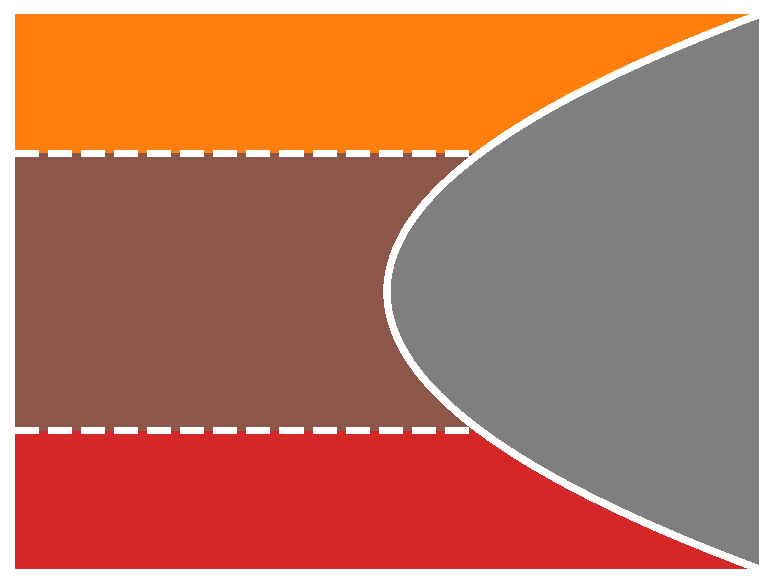
\includegraphics[width=0.38\textwidth]
            {gfx/ch-groundStateSymmetries/ground_states_polar_int_spin1.pdf}};
        \node[anchor=south west, inner sep=0] (rubidium) at (8, 0)
        {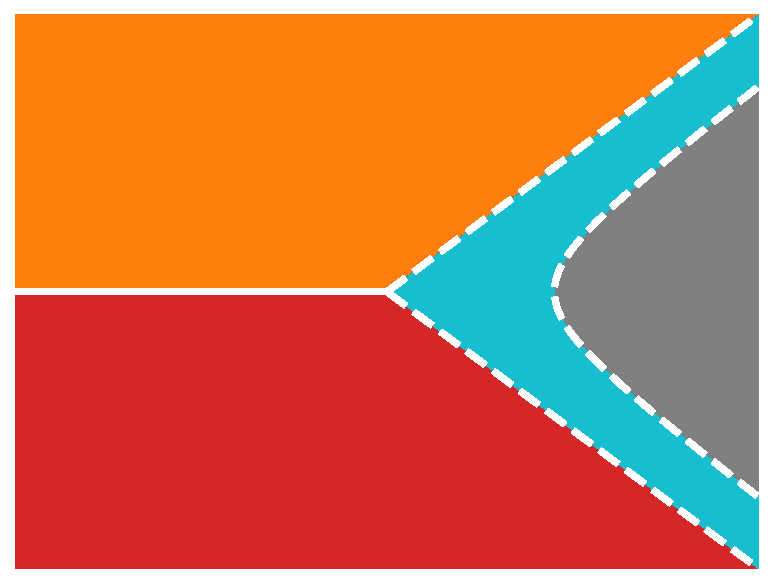
\includegraphics[width=0.38\textwidth]
            {gfx/ch-groundStateSymmetries/ground_states_fm_int_spin1.pdf}};

        \begin{scope}[x={($0.1*(sodium.south east)$)},
                y={($0.1*(sodium.north west)$)}]
            \draw[->, thick] (0,5)--(10.3,5) node[right]{$\frac{q}{c_1n}$};
            \draw[->, thick] (4.97,0)--(4.97,10.3) node[above]{$\frac{p}{c_1n}$};
            \draw[-] (6.1, 4.8) -- (6.1, 5.2);
            \node[anchor = south west] at (6.5, 3)
            {\scriptsize $p^2=2c_1nq$};
            \draw[->, thick] (6.6, 3.1) -- (6.25,2.55);
            \node at (4.8, 7.75) {\scriptsize $1$};
            \node at (4.7, 2.25) {\scriptsize -$1$};
            \node at (6.1, 4.5) {\scriptsize 1/2};
            \node[anchor=south west] at (0.5, 8.2)
            {\textcolor{white}{Ferromagnetic (I)}};
            \node[anchor=south west] at (0.5, 0.5)
            {\textcolor{white}{Ferromagnetic (II)}};
            \node[anchor=south west] at (0., 4.9)
            {\textcolor{white}{\small Antiferromagnetic}};
            \node[anchor=south west] at (2.1, 3.8)
            {\textcolor{white}{(III)}};
            \node[anchor=south west] at (6.5, 4.9)
            {\textcolor{white}{Polar (IV)}};
            \node[anchor=south west] at (3.8, -1.5) {\large $c_1 > 0$};
        \end{scope}
        \begin{scope}[x={($0.1*(sodium.south east)$)},
                y={($0.1*(sodium.north west)$)}]
            \draw[->, thick] (19.3,5)--(24.5,5) node[right]{$\frac{q}{|c_1|n}$};
            \draw[->, thick] (19.3,0)--(19.3,10.3) node[above]
            {$\frac{p}{|c_1|n}$};
            \node[anchor=south west] at (19.2, 8.6)
            {\scriptsize $p^2=q^2-2|c_1|nq$};
            \draw[->, thick] (19.7, 8.8) -- (21.9, 6.2);
            \node[anchor=south west, inner sep=0, rotate=-38] at (19.3, 4.)
            {\scriptsize $p=-q$};
            \node[anchor=south west, inner sep=0, rotate=38] at (19.5, 5.3)
            {\scriptsize $p=q$};
            \node[anchor=south west, inner sep=0] at (21.7, 4.5)
            {\scriptsize $2$};
            \node[anchor=south west] at (14.8, 6.5)
            {\textcolor{white}{Ferromagnetic (I)}};
            \node[anchor=south west] at (14.8, 1.5)
            {\textcolor{white}{Ferromagnetic (II)}};
            \node[anchor=south west] at (20.1, 4.9)
            {\textcolor{white}{BA}};
            \node[anchor=south west] at (20.1, 3.8)
            {\textcolor{white}{(V)}};
            \node[anchor=south west] at (22.1, 4.9)
            {\textcolor{white}{Polar}};
            \node[anchor=south west] at (22.1, 3.8)
            {\textcolor{white}{(IV)}};
            \node[anchor=south west] at (18., -1.5) {\large $c_1 < 0$};
        \end{scope}
    \end{tikzpicture}
    \caption[Spin-1 ground state phase diagram]
    {\label{fig: GS-phase-diagram}Ground state phase diagrams of spin-1
        BECs for polar (\(c_1 > 0\)) and ferromagnetic (\(c_1 < 0\))
        interactions in a parameter space of \((p, q)\).
        Solid or dashed white lines represent discontinuous and continuous phase
        transitions, respectively.}
\end{figure}
Fig.~\ref{fig: GS-phase-diagram} shows the ground state phase diagram for spin-1
BECs with \(c_1 > 0\) (left) and \(c_1 < 0\) (right) in the presence of a
magnetic field.
The full derivation of the ground state phase diagram can be found in recent
reviews~\cite{Kawaguchi2012, Stamper-Kurn2013}.
There are five total ground states shown in Fig.~\ref{fig: GS-phase-diagram},
which are summarised in Table~\ref{tab: spin-1-ground-states}.
\begin{table}
    \centering
    \begin{tabular}{ccc}
        \toprule
        Ground state                          & Spinor, \(\zeta^T\)                      & \(F_z\) \\
        \midrule
        Ferromagnetic (I)                     & \((1, 0, 0)\)                            & 1       \\
        Ferromagnetic (II)                    & \((0, 0, 1)\)                            & -1      \\
        Antiferromagnetic (III)               & \(\left(\sqrt{\frac{1 + p(c_1n)}{2}}, 0,
        \sqrt{\frac{1 - p(c_1n)}{2}}\right)\) & \(\frac{p}{c_1n}\)                                 \\
        Polar (IV)                            & \((0, 1, 0)\)                            & 0       \\
        Broken-axisymmetry (V)                & Eq.~\eqref{eq: BA-spinor}
                                              & \(\frac{p(-p^2+q^2+2qc_1n)}{2c_1nq^2}\)            \\
        \bottomrule
    \end{tabular}
    \caption{\label{tab: spin-1-ground-states}Summary of the ground state
        phases in a spin-1 BEC with their respective spinors and magnetisation.}
\end{table}

There exists a fully magnetised ferromagnetic state with \(\zeta={(1, 0, 0)}^T\)
and \(F_z=1\) (state I) or \(\zeta={(0, 0, 1)}^T\) and \(F_z=-1\) (state II),
depending on the sign of the linear Zeeman shift \(p\).
A non-magnetised polar phase (state IV) arises with \(\zeta={(0, 1, 0)}^T\) and
\(F_z = 0\).
For polar interactions \(c_1 > 0\), there exists an antiferromagnetic phase
(state III) with
\begin{equation}\label{eq: AFM-spinor}
    \zeta^\mathrm{AFM} = {\left(\sqrt{\frac{1 + p/(c_1n)}{2}}, 0,
    \sqrt{\frac{1 - p/(c_1n)}{2}}\right)}^T,
\end{equation}
and \(F_z = p/(c_1n)\).
At \(p=0\), this state transforms into the easy-plane polar phase, i.e., state
IV with the nematic director in the \(xy\)-plane.
Finally, a broken-axisymmetry (BA) phase (state V) occurs in a condensate with
\(c_1 > 0\) which has a spinor of the form
\begin{equation}
    \begin{aligned}
        \zeta_{\pm 1} & =
        \frac{q \pm p}{2q}\sqrt{\frac{-p^2+q^2+2c_1nq}{2c_1nq}},              \\
        \zeta_0       & = \sqrt{\frac{(q^2-p^2)(-p^2-q^2+2c_1nq)}{4c_1nq^3}},
    \end{aligned}
    \label{eq: BA-spinor}
\end{equation}
which has a magnetisation that tilts against the quantisation axis
\begin{equation}
    F_z = \frac{p(-p^2 + q^2 + 2qc_1n)}{2c_1nq^2}.
\end{equation}
These five ground states fully encapsulate the phase diagram of spin-1 BECs
in a magnetic field.

\subsection{Graphical representation of spin-1 ground states}
Graphical representations help us to visual the symmetry properties of different
ground states in spinor systems.
In particular, they can provide valuable insight to what is occurring within
the order parameter when, e.g., topological defects form or the symmetry of the
system is spontaneously broken.
Here we focus on two types of graphical representation: Spherical harmonics and
Majorana representations.
Spherical harmonics in particular are widely used in Chapter~\ref{chap: spin-2},
where the system exhibits multiple ground states, and hence different symmetries
at once.

\subsubsection{Spherical harmonic representation}
We first consider the spherical harmonic representation, which maps the
order parameter onto spherical harmonics using the relation
\begin{equation}
    Z(\hat{s}) = \sum_m\zeta_m Y_f^m(\hat{s}),
    \label{eq: spherical-harmonics}
\end{equation}
where \(\hat{s}\) is a unit vector in 3D spin space, and \(Y_f^m \) are the
spherical harmonics for a spin-\(f\) state.
The symmetry can be visualised with a surface plot of \(|Z(\hat{s})|^2\),
where the surface colour is represented by the argument of \(Z(\hat{s})\).

The orientation of the spherical harmonics corresponds to the condensate spin,
and so as the spin vector rotates, the orientation of spherical harmonics
rotates to match.
In addition, the colour of the spherical harmonics corresponds to the global
phase, \( \tau \).
Therefore, the spherical harmonics give an accurate description of the
physical symmetries of the wave function, along with a pictorial representation
of how the phase is changing.
Throughout this thesis we will use the spherical harmonics to construct a
picture of what is happening to the wave function at different locations in
space, where the symmetry of the wave function can rapidly transform in a
non-trivial manner (see Chapter~\ref{chap: spin-2}).

In spin-1, there are three \(f = 1\) spherical harmonics given by
\begin{align}
    Y_1^0(\theta, \phi)       & = \frac{1}{2}\sqrt{\frac{3}{\pi}}\cos\theta, \\
    Y_1^{\pm 1}(\theta, \phi) & =
    \frac{1}{2}\sqrt{\frac{3}{2\pi}}e^{\pm i \phi}\sin\theta.
\end{align}
The spherical harmonic representations of the spin-1 polar and ferromagnetic
ground states are shown in Fig.~\ref{fig: spin-1-spherical-harmonics}.
\begin{figure}
    \begin{tikzpicture}
        % Plots
        \node at (0, 0) {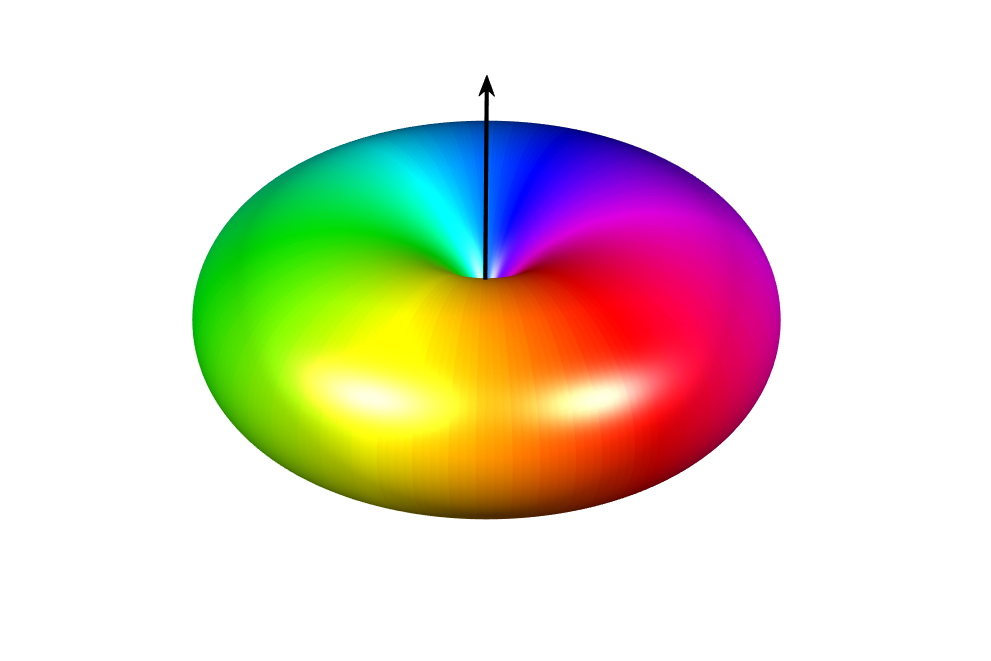
\includegraphics[width=0.49\textwidth]
            {gfx/ch-groundStateSymmetries/FM-spherical.pdf}};
        \node at (7.2, 0) {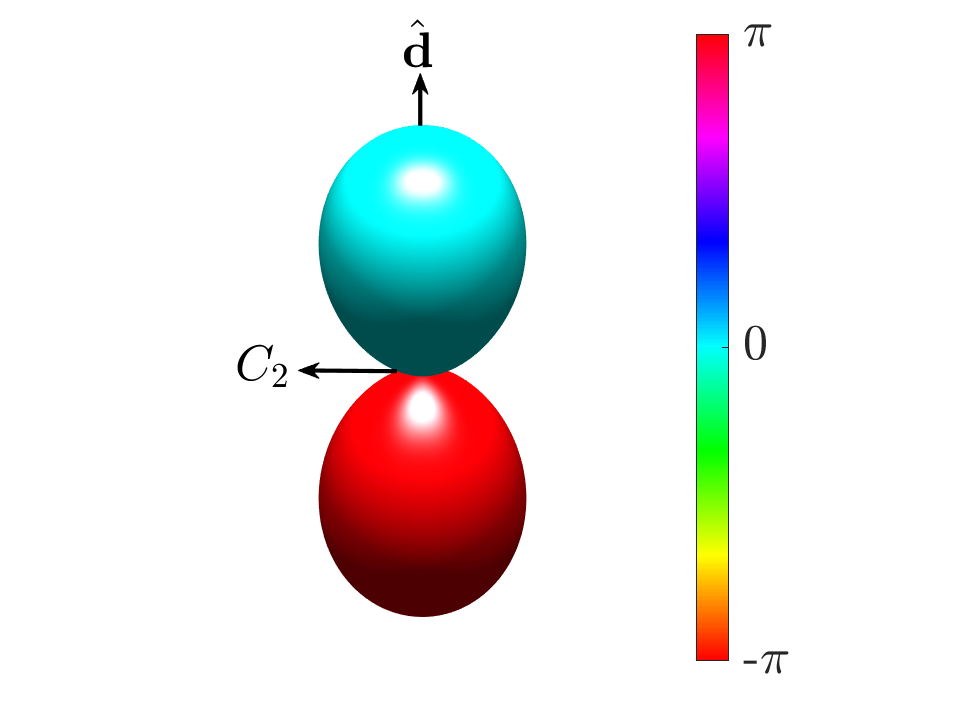
\includegraphics[scale=0.55]
            {gfx/ch-groundStateSymmetries/polar-spherical.pdf}};
        \node at (0, -5) {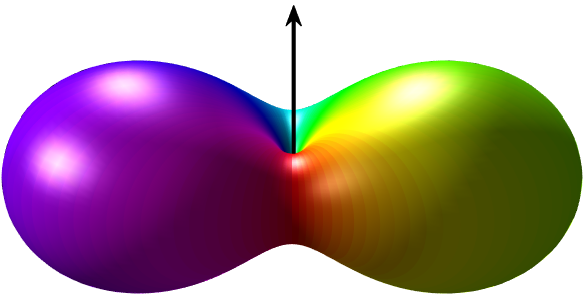
\includegraphics[width=0.49\textwidth]
            {gfx/ch-groundStateSymmetries/AFM-spherical.pdf}};
        \node at (7.2, -5) {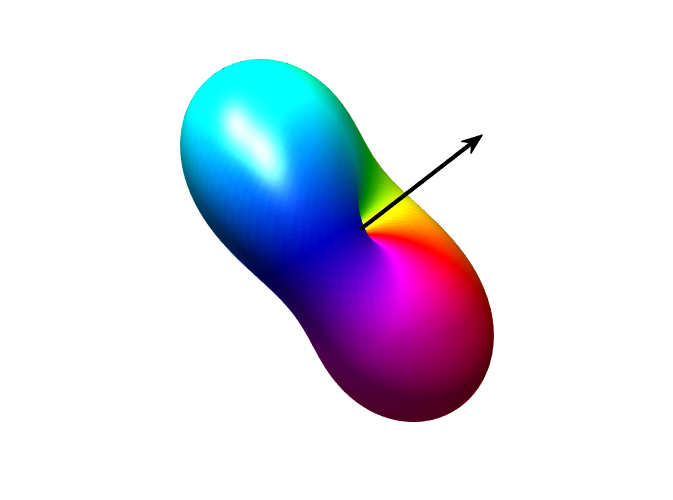
\includegraphics[width=0.49\textwidth]
            {gfx/ch-groundStateSymmetries/BA-spherical.pdf}};

        % Colour bar
        \node at (4, 0) {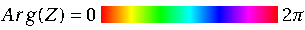
\includegraphics[angle=90]
            {gfx/colourbars/compiled_hsv.pdf}};

        % Labels
        \node at (0, -2.) {(a)};
        \node at (7.2, -2.) {(b)};
        \node at (0, -7.2) {(c)};
        \node at (7.2, -7.2) {(d)};

        % Spinors
        \node at (0, 3) {\(\zeta^\mathrm{FM}={(1, 0, 0)}^T\)};
        \node at (7.2, 3) {\(\zeta^\mathrm{P}={(0, 1, 0)}^T\)};
        \node at (0, -2.5) {\(\zeta^\mathrm{AFM} \) given in
            Eq.~\eqref{eq: AFM-spinor}};
        \node at (7.2, -2.5) {\(\zeta^\mathrm{BA}\) given in
            Eq.~\eqref{eq: BA-spinor}};

    \end{tikzpicture}
    \caption[Spherical harmonic representation of spin-1 ground states]
    {\label{fig: spin-1-spherical-harmonics}
    Spherical harmonics representation of the ground state phases available in a
    spin-1 BEC.\@
    (a): The spin-1 ferromagnetic ground state with
    \(\zeta^\mathrm{FM}={(1, 0, 0)}^T\).
    The black arrow represents the direction of the condensate magnetisation.
    (b): The spin-1 polar ground state with
    \(\zeta^\mathrm{P}={(0, 1, 0)}^T\) where the nematic director
    \(\hat{\vb{d}}\) is aligned with the \(z\)-axis.
    The order parameter remains unchanged about \(\pi/2\) rotations about the
    \(C_2\) axis.
    (c): The anti-ferromagnetic state given by Eq.~\eqref{eq: AFM-spinor}.
    Note that for this state the direction of the spin vector is aligned with
    the magnetic field.
    (d): The broken-axisymmetry state given by Eq.~\eqref{eq: BA-spinor}.
    The direction of the spin is tilted away from the magnetic field axis.
    \textcolor{red}{Would like this on one row, like spin-2 paper.}}
\end{figure}
We see that the ferromagnetic order parameter has an \(SO(2)\) symmetry about
the \(z\)-axis.
The polar state has two nematic lobes which have a \(\pi \) phase difference.
These lobes are aligned along an axis of symmetry given by the nematic director,
\(\hat{\vb{d}}\).
There is a further axis of symmetry about the \(C_2\) axis, about which \(\pi \)
rotations preserve the symmetry.

\subsubsection{Majorana representation}
An alternative description to visualising the symmetries of spinor BECs is
through the use of the Majorana representation~\cite{Majorana1932,Bloch1945},
where a spin-\(f\) system can be represented as \(2f\) points on the Bloch
sphere.
The points on the sphere are numerically calculated as the \(2f\) roots
\(z_j\) of the polynomial equation
\begin{equation}
    P^{(f)}(z) = \sum_{\alpha = 0}^{2f}
    \sqrt{\mqty(2f \\ \alpha)}\zeta_{f-\alpha}^*z^\alpha=0,
\end{equation}
where each root represents a stereographic mapping
\(z_j=\tan(\theta/2)e^{i\phi}\) of the spherical coordinates \((\theta, \phi)\).
For the spin-1 system, the polynomial is
\begin{equation}
    P^{(1)}(z) = \zeta_1^*z^2+\sqrt{2}\zeta_0^*z+\zeta_{-1}^*.
\end{equation}
The disadvantage of this representation is that one is not able to see the
condensate phase.
The equivalent Majorana representations for the states shown in
Fig.~\ref{fig: spin-1-spherical-harmonics} are shown in
Fig.~\ref{fig: spin-1-majorana}.
\begin{figure}
    \centering
    \begin{tikzpicture}
        \node at (0, 0){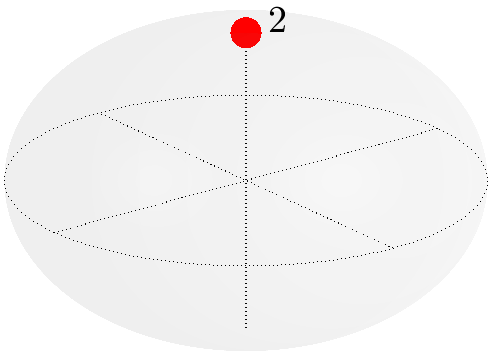
\includegraphics[width=0.3\textwidth]
            {gfx/ch-groundStateSymmetries/FM-Majorana.pdf}};
        \node at (4.5, 0){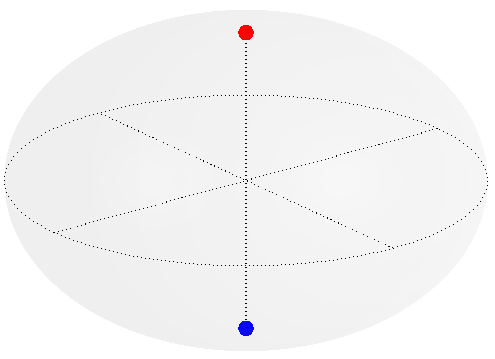
\includegraphics[width=0.3\textwidth]
            {gfx/ch-groundStateSymmetries/polar-Majorana.pdf}};
        \node at (9, 0){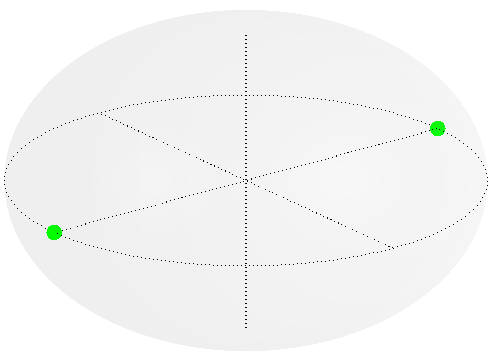
\includegraphics[width=0.3\textwidth]
            {gfx/ch-groundStateSymmetries/AFM-Majorana.pdf}};
        \node at (11.8, 0) {
            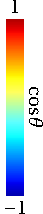
\includegraphics{gfx/colourbars/compiled_jet_majorana.pdf}};

        \node at (0, -2) {(a)};
        \node at (4.5, -2) {(b)};
        \node at (9, -2) {(c)};

        \node at (0, 2) {\(\zeta={(1, 0, 0)}^T\)};
        \node at (4.5, 2) {\(\zeta={(0, 1, 0)}^T\)};
        \node at (9, 2) {\(\zeta={(1, 0, 1)}^T/\sqrt{2}\)};
    \end{tikzpicture}
    \caption[Majorana representation of spin-1 ground states]
    {\label{fig: spin-1-majorana}Majorana representations of spin-1 ground
    states. The colour of the points represent \(\cos\theta =
    (1-|z|^2)/(1+|z|^2)\).
    A number next to a point represents the root when the polynomial
    \(P_\psi^1(z)\) has an \(n\)-multiple root.
    (a): Ferromagnetic state with \(\zeta={(1, 0, 0)}^T\).
    (b): Polar state with \(\zeta={(0, 1, 0)}^T\).
    (c): AFM state with \(\zeta={(1, 0, 1)}^T/\sqrt{2}\).}
\end{figure}

\section{Ground states of spin-2 BECs}\label{sec: ground-states-spin-2}
To find the ground states of a spin-2 system we follow a similar procedure to
the spin-1 case.
The interacting part of the spin-2 Hamiltonian reads
\begin{align}
    E_\mathrm{int} = \frac{1}{2}\int c_0n^2 + c_1|\vb{F}|^2+c_2|A_{20}|^2
    d\vb{r}.
\end{align}
As before, the density remains fixed for any normalised ground state and so
different ground states arise from the competition between the spin-
and singlet-dependent interaction strengths.

\subsection{Ferromagnetic phase}
If we first consider \(c_1 < 0\) and \(c_2 > 0\), then the energy functional is
minimised when  the spin density is maximised \(\spinmag=2\)
and the singlet-duo amplitude is minimised \(|A_{20}|=0\).
This state is denoted as the spin-2 ferromagnetic phase, where \(\spinmag \) is
now \(\spinmag=2\) for this ground state, as opposed to \(\spinmag=1\) in the
spin-1 system.
Note that there exists a ferromagnetic state in a spin-2 BEC with
\(\spinmag=1\), but this state is not the ground state since the \(\spinmag=2\)
state has lower energy.
To avoid confusion, we refer to the ferromagnetic state with \(\spinmag=2\) as
the FM-2 state, and the state with \(\spinmag=1\) as the FM-1 state.
It should be noted, however, that the FM-1 state can remain stable in
certain situations, such as in the cores of vortices (see
Chapter~\ref{chap: spin-2}).
The representative spinors for the spin-2 ferromagnetic states have the form
\begin{equation}
    \zeta^\mathrm{FM-2} = \mqty(1 \\ 0 \\ 0 \\ 0 \\ 0), \qquad
    \zeta^\mathrm{FM-1} = \mqty(0 \\ 1 \\ 0 \\ 0 \\ 0).
\end{equation}

As in the spin-1 case, the energy of a given spinor in the absence of a magnetic
field is degenerate following the application of a global \(U(1)\) phase and an
\(SO(3)\) spin rotation.
In a spin-2 system, a general spin rotation is instead represented as a
\(5\times 5\) matrix of the form
\begin{multline}\label{eq: spin-2-rotation-matrix}
    U(\alpha, \beta, \gamma) = \\
    \scalemath{0.90}{\mqty(
    e^{-2i(\alpha + \gamma)}C^4 & -2e^{-i(2\alpha+\gamma)}C^3S
    & \sqrt{6}e^{-2i\alpha}C^2S^2 & -2e^{-i(2\alpha-\gamma)}CS^3
    & e^{-2i(\alpha + \gamma)}S^4
    \\
    2e^{-i(\alpha+2\gamma)}C^3S & e^{-i(\alpha+\gamma)}C^2(C^2-3S^2)
    & -\sqrt{\frac{3}{8}}e^{-i\alpha}\sin 2\beta
    & -e^{-i(\alpha-\gamma)}S^2(S^2-3C^2) & -2e^{-i(\alpha-2\gamma)}CS^3
    \\
    \sqrt{6}e^{-2i\gamma}C^2S^2 & \sqrt{\frac{3}{8}}e^{-i\gamma}\sin 2\beta
    & \frac{1}{4}(1+3\cos 2\beta)
    & -\sqrt{\frac{3}{8}}e^{-i\gamma}\sin 2\beta
    & \sqrt{6}e^{2i\gamma}C^2S^2
    \\
    2e^{i(\alpha-2\gamma)}CS^3 & -e^{i(\alpha-\gamma)}S^2(S^2-3C^2)
    & \sqrt{\frac{3}{8}}e^{i\alpha}\sin 2\beta
    & e^{i(\alpha-\gamma)}C^2(C^2-3S^2) & -2e^{i(\alpha+2\gamma)}C^3S
    \\
    e^{2i(\alpha - \gamma)}C^4 & 2e^{i(2\alpha-\gamma)}CS^3
    & \sqrt{6}e^{2i\alpha}C^2S^2 & 2e^{i(2\alpha+\gamma)}C^3S
    & e^{2i(\alpha + \gamma)}C^4
    )},
\end{multline}
where \(S \equiv \sin(\beta/2)\) and \(C \equiv \cos(\beta/2)\).
Following the same procedure as the spin-1 case and applying the above spin
rotation with a global phase \(\tau \) and condensate density \(n\) yields the
general FM-2 wave function
\begin{equation}\label{eq: FM-2-representative-spinor}
    \psi^\mathrm{FM} = \sqrt{n}e^{i\tau'}\mqty(
    e^{-2i\alpha} \cos^4\frac{\beta}{2} \\
    2e^{-i\alpha}\cos^3\frac{\beta}{2}\sin \frac{\beta}{2} \\
    \sqrt{6} \cos^2\frac{\beta}{2} \sin^2\frac{\beta}{2} \\
    2e^{i\alpha}\cos\frac{\beta}{2} \sin^3\frac{\beta}{2} \\
    e^{2i\alpha} \sin^4\frac{\beta}{2}
    ),
\end{equation}
where \(\tau'=\tau-2\gamma \).

\subsection{Nematic phases}
Instead, let us now consider the case of \(c_1 > 0\) and \(c_2 < 0\).
We see that the energy functional is minimised when the spin is minimised
\(\spinmag = 0\) but the singlet-duo amplitude is maximised
\(|A_{20}|^2 = n/5\).
Such a state is called nematic, and takes two forms: the uniaxial nematic (UN)
or biaxial nematic (BN), described by the spinors
\begin{equation}
    \zeta^\mathrm{UN} = \mqty(0 \\ 0 \\ 1 \\ 0 \\ 0), \qquad
    \zeta^\mathrm{BN} = \frac{1}{\sqrt{2}}\mqty(1 \\ 0 \\0 \\ 0 \\ 1).
\end{equation}
In the absence of a magnetic field, these two states are degenerate.
The general wave function for the UN state is
\begin{equation}\label{eq: UN-representative-spinor}
    \psi^\mathrm{UN} = \frac{\sqrt{6n}}{4}e^{i\tau}\mqty(
    e^{-2i\alpha} \sin^2\beta \\
    -2e^{-i\alpha} \sin\beta \cos\beta \\
    \sqrt{\frac{2}{3}}(3\cos^2\beta - 1) \\
    2e^{i\alpha} \sin\beta \cos\beta \\
    e^{2i\alpha} \sin^2\beta
    ),
\end{equation}
and for the BN
\begin{equation}\label{eq: BN-representative-spinor}
    \psi^\mathrm{BN} = \sqrt{\frac{n}{2}}e^{i\tau} \mqty(
    e^{-2i\alpha}\left[\left(1 - \frac{1}{2}\sin^2\beta\right)\cos 2\gamma
        - i\cos\beta\sin 2\gamma\right] \\
    e^{-i\alpha}\sin\beta(\cos\beta\cos 2\beta - i\sin 2\gamma) \\
    \sqrt{\frac{3}{2}}\sin^2\beta \cos 2\gamma \\
    -e^{i\alpha}\sin\beta(\cos\beta\cos 2\gamma + i\sin 2\gamma) \\
    e^{2i\alpha}\left[\left(1 - \frac{1}{2}\sin^2\beta\right)\cos 2\gamma
        + i\cos\beta\sin 2\gamma\right]
    ).
\end{equation}

\subsection{Cyclic phase}
Now consider \(c_1, c_2 > 0\).
The energy functional is minimised when both the spin magnitude and singlet-duo
amplitude is minimised: \(\spinmag = 0, |A_{20}|^2=0\).
Such a state is referred to as the cyclic state and has the representative
spinor
\begin{equation}
    \zeta^\mathrm{C-1} = \frac{1}{2}\mqty(1 \\ 0 \\ i\sqrt{2} \\ 0 \\ 1).
    \label{eq: C-1-spinor}
\end{equation}
The general wave function is given as
\begin{equation}
    \psi^\mathrm{C} = \frac{\sqrt{n}}{2}e^{i\tau} \mqty(
    e^{-2i(\alpha+\gamma)}C^4 + 2i\sqrt{3}e^{-2i\alpha}C^2S^2
    + e^{-2i(\alpha-\gamma)}S^4
    \\
    2e^{-i(\alpha+2\gamma)}C^3S - \frac{\sqrt{3}}{2}ie^{-i\alpha}\sin 2\beta
    - 2e^{-i(\alpha-2\gamma)}CS^3
    \\
    \sqrt{6}e^{-2i\gamma}C^2S^2 + i\frac{\sqrt{2}}{4}(1+3\cos 2\beta)
    + \sqrt{6}e^{2i\gamma}C^2S^2
    \\
    2e^{i(\alpha-2\gamma)}CS^3 + \frac{\sqrt{3}}{2}ie^{i\alpha}\sin 2\beta
    - 2e^{i(\alpha+2\gamma)}C^3S
    \\
    e^{2i(\alpha-\gamma)}S^4 + 2i\sqrt{3}e^{2i\alpha}C^2S^2
    + e^{2i(\alpha+\gamma)}C^4
    ).
\end{equation}
In addition to the three-component cyclic state, there is also a two-component
cyclic state that is useful for understanding the general cyclic state:
\begin{equation}
    \zeta^\mathrm{C-2} = \frac{1}{\sqrt{3}}\mqty(1  \\ 0 \\ 0 \\ \sqrt{2} \\ 0),
    \label{eq: C-2-spinor}
\end{equation}
which is obtained from Eq.~\eqref{eq: C-1-spinor} via the spin
rotation~\cite{Kawaguchi2012}
\begin{equation}
    \zeta^{C-2} = -ie^{i\frac{\pi}{4}\hat{F}_z}
    \exp\left[i\frac{\hat{F}_x-\hat{F}_y}{\sqrt{2}}
        \arccos{\left(\frac{1}{\sqrt{3}}\right)}\right]\zeta^\mathrm{C-1}.
\end{equation}
The ground states of the spin-2 system in a parameter space of \((c_1, c_2)\)
are summarised in Fig.~\ref{fig: spin-2-ground-states}.
\begin{figure}
    \centering
    \begin{tikzpicture}
        \node[anchor=south west, inner sep=0] (diagram) at (0, 0)
        {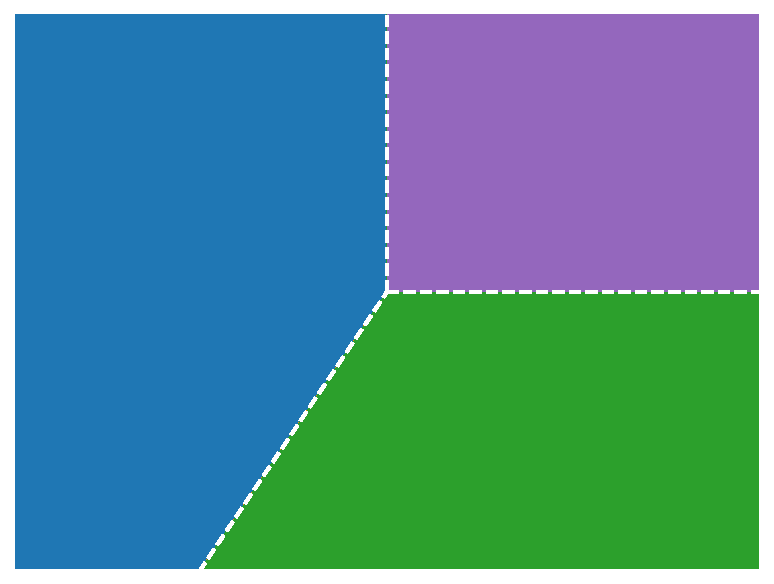
\includegraphics[width=0.5\textwidth]
            {gfx/ch-groundStateSymmetries/ground_states_spin2.pdf}};
        \begin{scope}[x={($0.1*(diagram.south east)$)},
                y={($0.1*(diagram.north west)$)}]
            \draw[->, thick, anchor=south west] (9.8, 5) -- (10.1, 5)
            node[right] {$c_1n$};
            \draw[->, thick, anchor=south west] (5, 9.7) -- (5, 10.1)
            node[above] {$c_2n$};
            \draw[-, thick, anchor=south west] (0.21, 5) -- (4.98, 5);
            \node at (7.5, 7) {\textcolor{white}{Cyclic}};
            \node at (2.5, 7) {\textcolor{white}{Ferromagnetic}};
            \node at (7, 2) {\textcolor{white}{Nematic}};
            \node[anchor=south east] at (5, 5) {\textcolor{white}{0}};
            \node[anchor=south west, rotate=53] at (2.7, 0.7)
            {\textcolor{white}{\(c_2n=20c_1n\)}};
        \end{scope}
    \end{tikzpicture}
    \caption[Spin-2 ground state phase diagram]
    {\label{fig: spin-2-ground-states}Ground state phase diagram for
        spin-2 BECs in a parameter space of \((c_1, c_2)\) in the absence of a
        magnetic field.
        White dashed lines indicate a first-order phase transition region
        between the phases.}
\end{figure}
Note, for the case of \(c_1, c_2 < 0\), there is a competition between
the ferromagnetic and nematic phases.
For this case the energy functional is minimised by either having maximal spin
density and \(|A_{20}|^2 = 0\) as in the ferromagnetic phase, or by having
minimal spin density and \(|A_{20}|^2 = n/5\) as in the nematic phase, which
leads to a phase boundary at \(c_2n=20c_1n\).

\subsection{Graphical representation of spin-2 ground states}
\subsubsection{Spherical harmonic representation}
The mapping of the order parameter onto spherical harmonics in the spin-2 case
follows the same equation as in the spin-1 case, i.e.,
Eq.~\eqref{eq: spherical-harmonics}.
For the spin-2 system, however, we have five \(f=2\) spherical harmonics given
by
\begin{align}
    Y_2^0(\theta, \phi)       & = \frac{1}{4}\sqrt{\frac{5}{\pi}}
    (3\cos^2\theta - 1),                                                    \\
    Y_2^{\pm 1}(\theta, \phi) & =
    \mp \frac{1}{2}\sqrt{\frac{15}{2\pi}}e^{\pm i\phi}\sin\theta\cos\theta, \\
    Y_2^{\pm 2}(\theta, \phi) & =
    \frac{1}{4}\sqrt{\frac{15}{2\pi}}e^{\pm 2i\phi}\sin^2\theta.
\end{align}
The spherical harmonics for the ferromagnetic, UN, BN, and cyclic states
are shown in Fig.~\ref{fig: spin-2-spherical-harmonics}.
\begin{figure}
    \centering
    \begin{tikzpicture}
        % Plots
        \node at (0, 0) {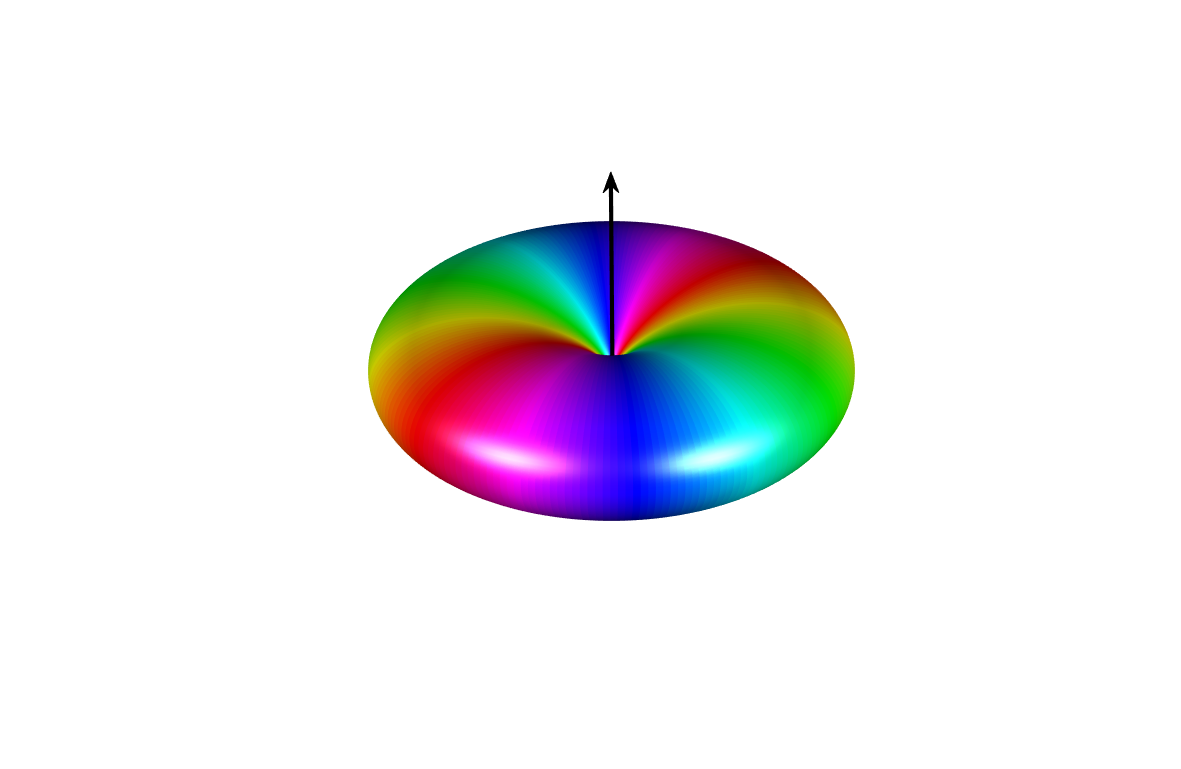
\includegraphics[width=0.45\textwidth]
            {gfx/ch-groundStateSymmetries/FM-2-spherical.pdf}};
        \node at (7.2, 0) {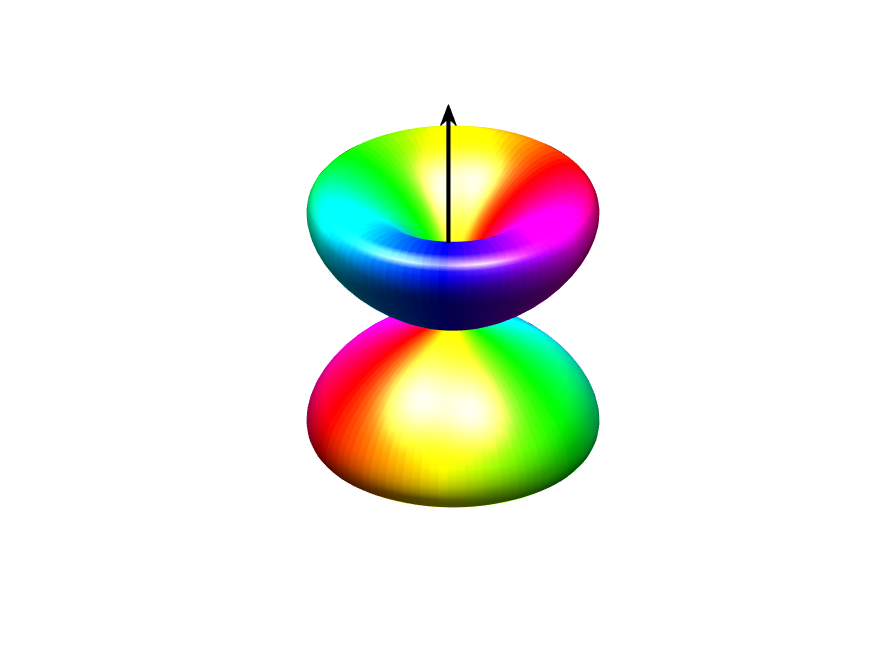
\includegraphics[width=0.45\textwidth]
            {gfx/ch-groundStateSymmetries/FM-1-spherical.pdf}};
        \node at (0, -6) {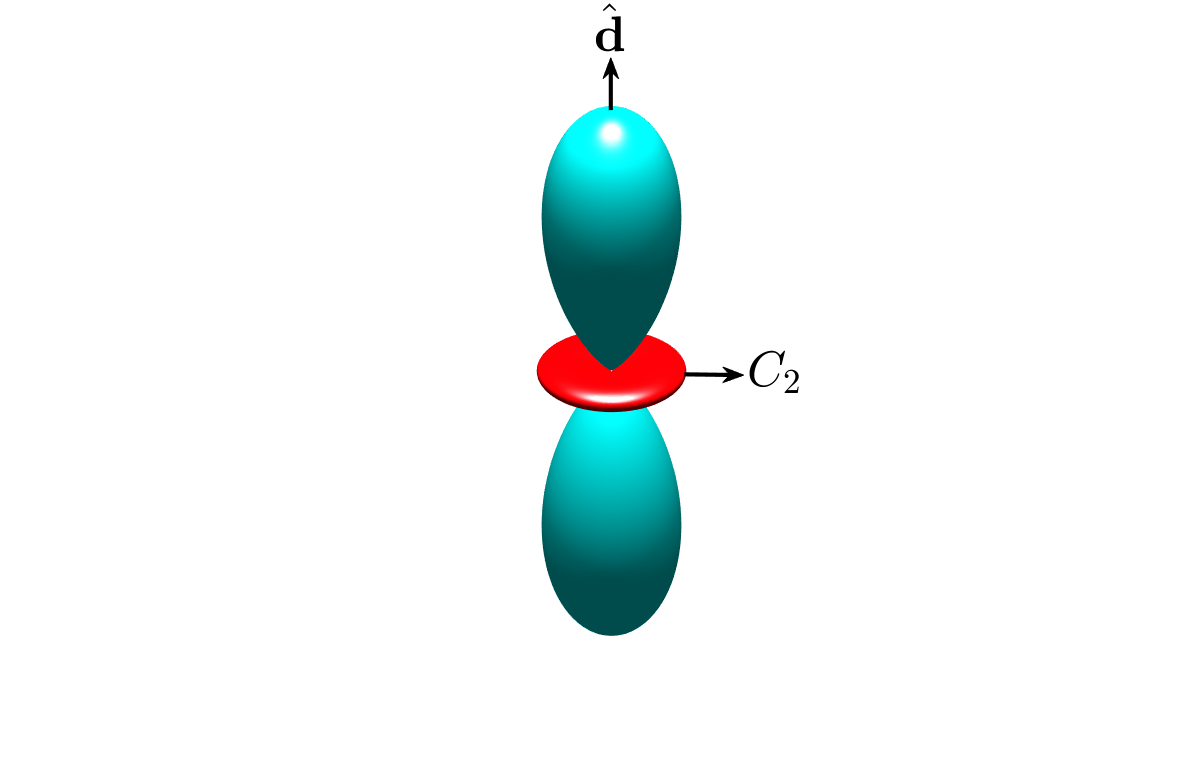
\includegraphics[width=0.45\textwidth]
            {gfx/ch-groundStateSymmetries/UN-spherical.pdf}};
        \node at (7.2, -6) {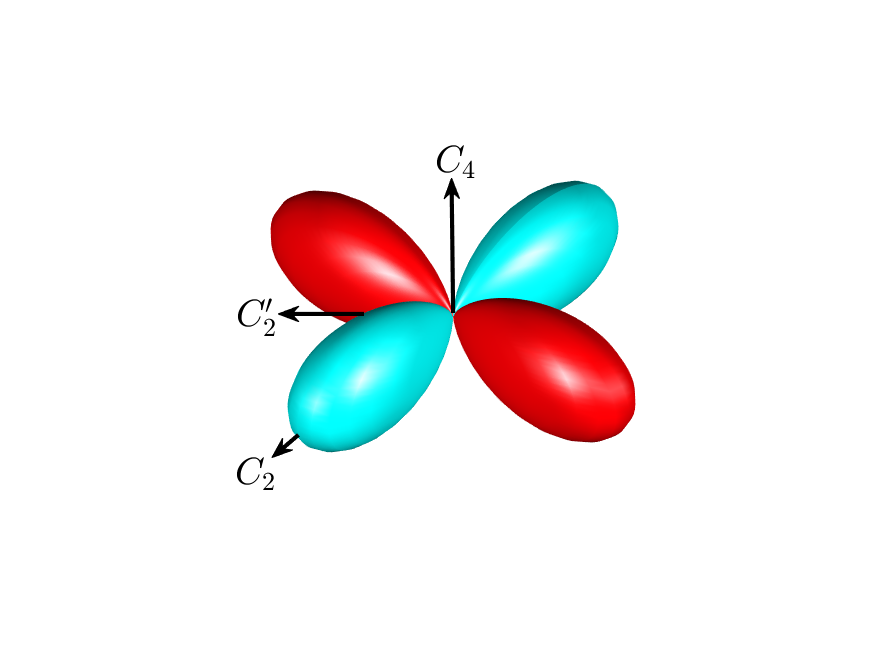
\includegraphics[width=0.45\textwidth]
            {gfx/ch-groundStateSymmetries/BN-spherical.pdf}};
        \node at (0, -12) {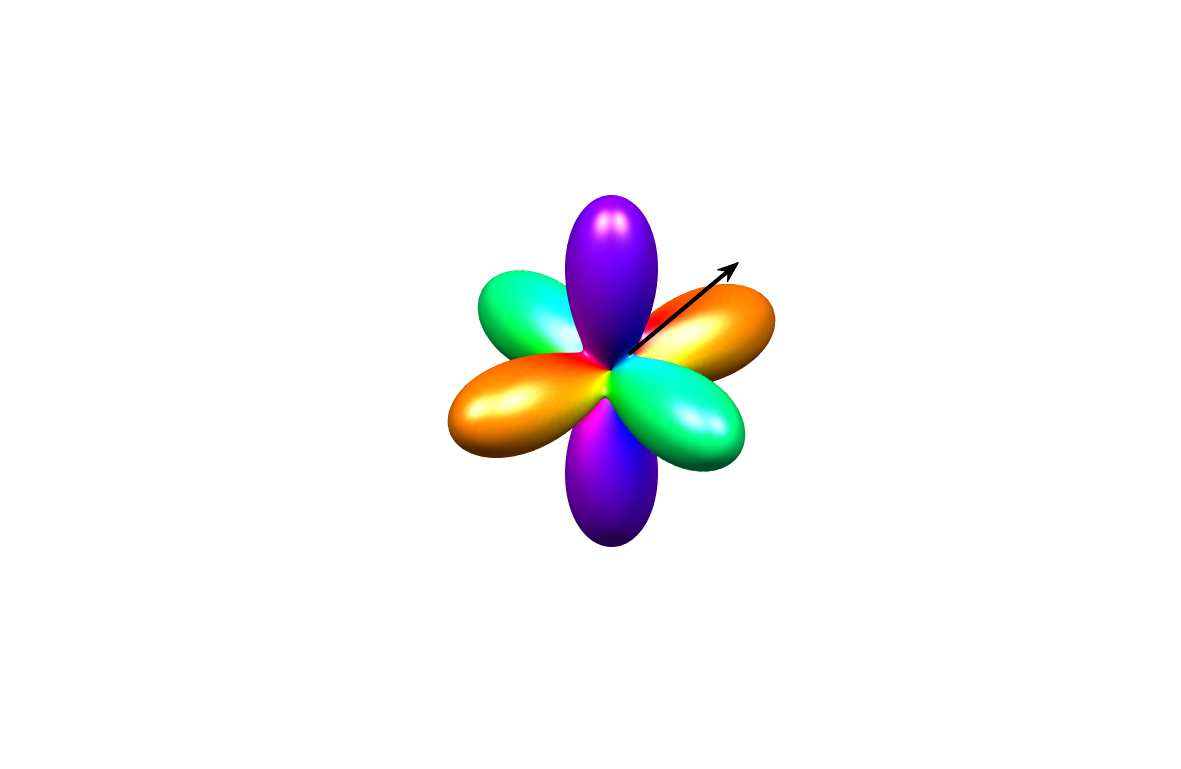
\includegraphics[width=0.45\textwidth]
            {gfx/ch-groundStateSymmetries/C1-spherical.pdf}};
        \node at (7.2, -12) {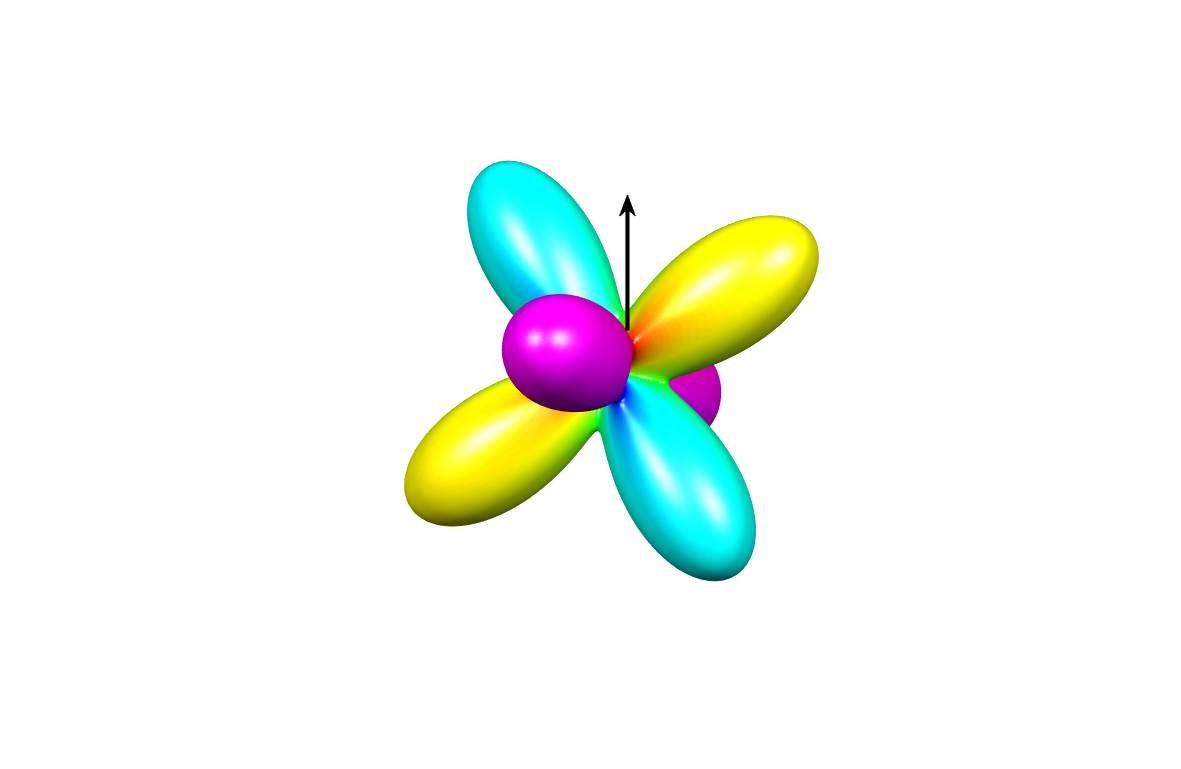
\includegraphics[width=0.45\textwidth]
            {gfx/ch-groundStateSymmetries/C2-spherical.pdf}};

        % Colour bars
        \node at (3.2, -13.6) {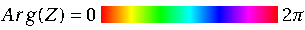
\includegraphics{gfx/colourbars/compiled_hsv.pdf}};

        % Labels
        \node at (0, -2) {(a)};
        \node at (7.2, -2) {(b)};
        \node at (0, -8) {(c)};
        \node at (7.2, -8) {(d)};
        \node at (0, -14) {(e)};
        \node at (7.2, -14) {(f)};

        % Spinors
        \node at (0, 2.5) {\(\zeta={(1, 0, 0, 0, 0)}^T\)};
        \node at (7.2, 2.5) {\(\zeta={(0, 1, 0, 0, 0)}^T\)};
        \node at (0, -3.2) {\(\zeta={(0, 0, 1, 0, 0)}^T\)};
        \node at (7.2, -3.2) {\(\zeta={(1, 0, 0, 0, 1)}^T/\sqrt{2}\)};
        \node at (0, -9.5) {\(\zeta={(1, 0, i\sqrt{2}, 0, 1)}^T/2\)};
        \node at (7.2, -9.5) {\(\zeta={(\sqrt{1/3}, 0, 0, \sqrt{2/3}, 0)}^T\)};
    \end{tikzpicture}
    \caption[Spherical harmonic representation of spin-2 ground states]
    {\label{fig: spin-2-spherical-harmonics}Spherical harmonic
        representations for different ground states in a spin-2 system.
        (a) and (b): Ferromagnetic states with a spin of \(|F|=2n\) and
        \(|F|=n\), respectively, where the arrows indicate the direction of
        magnetisation.
        (c): the uniaxial nematic state where \(\hat{\vb{d}}\) is the nematic
        director. The order parameter remains unchanged about \(\pi \) rotations
        about the \(C_2\) axis.
        (d): the biaxial nematic state. The order parameter is symmetric under
        \(\pi/2\) rotations about the \(C_4\) axis.
        Additionally, there is a two-fold symmetry about the \(C_2, C_2'\) axes.
        (e) and (f): the cyclic states which have a two- and three-fold symmetry
        about the \(C_2, C_3\) axes, respectively.
        \textcolor{red}{Add \(C_2'\) axis in (e) for use in spin-2 chapter.}
    }
\end{figure}
It is clear from Figs~\ref{fig: spin-2-spherical-harmonics}a
and~\ref{fig: spin-2-spherical-harmonics}b that the ferromagnetic order
parameters have the same \(SO(2)\) symmetry about the \(z\)-axis as the spin-1
case.
However, the difference between the FM-2 phase of the spin-2 system and the FM
phase of the spin-1 system is apparent in the phase: the FM-2 state winds by
\(4\pi \) about the spherical harmonic as opposed to \(2\pi \)
(see Fig.~\ref{fig: spin-1-spherical-harmonics}a).

The UN phase as shown in Fig.~\ref{fig: spin-2-spherical-harmonics}c differs
slightly from the polar phase of spin-1 (see
Fig.~\ref{fig: spin-1-spherical-harmonics}b) in that the nematic lobes have the
same phase.
This implies that a \(\pi \) spin rotation about any axis in the \(xy\)-plane
leaves the order parameter unchanged.
In addition, like the ferromagnetic states, this order parameter also has an
\(SO(2)\) symmetry about the \(z\)-axis.

The BN phase, shown in Fig.~\ref{fig: spin-2-spherical-harmonics}d, breaks the
\(SO(2)\) symmetry due to the perpendicular nematic lobes, which have a \(\pi \)
phase difference.
The symmetry of the order parameter is preserved under \(\pi/4\) rotations
about the \(C_4\) axis.
In addition, the BN order parameter is invariant under \(\pi \) rotations about
both the \(C_2\) and \(C_2'\) axes.

Finally, the cyclic order parameter, shown in
Figs.~\ref{fig: spin-2-spherical-harmonics}e
and~\ref{fig: spin-2-spherical-harmonics}f, have the symmetry of a tetrahedron.
Each nematic lobe has a two-fold symmetry about the \(C_2\) axis.
Furthermore, the order parameter has a three-fold symmetry about the \(C_3\)
axis.
In Fig.~\ref{fig: spin-2-spherical-harmonics}e, this axis is the
\((1, 1, 1)\)-axis, whereas in Fig.~\ref{fig: spin-2-spherical-harmonics}f,
it is aligned along the \(z\)-axis.
Rotations of \(2\pi/3\) about this axis preserve the symmetry of the order
parameter.

\subsubsection{Majorana representation}
The mapping of the spin-2 system onto the Majorana representation follows a
similar procedure to the spin-1 case.
In this system, we compute the \(2f=4\) roots of the complex polynomial
\begin{equation}
    P^{(2)}(z) = \zeta_2^*z^4 + 2\zeta_1^*z^3 + \sqrt{6}\zeta_0^*z^2
    + 2\zeta_{-1}^*z + \zeta_{-2}^*.
\end{equation}
The Majorana representation of the ferromagnetic, UN, BN, and cyclic states
are shown in Fig.~\ref{fig: spin-2-Majorana}.
\begin{figure}
    \centering
    \begin{tikzpicture}
        % First row
        \node at (0, 0){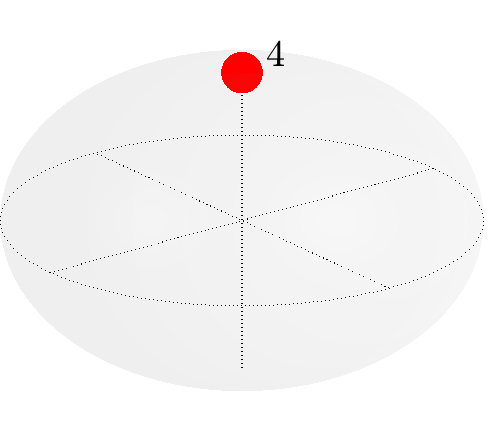
\includegraphics[width=0.3\textwidth]
            {gfx/ch-groundStateSymmetries/FM-2-Majorana.pdf}};
        \node at (4.5, 0){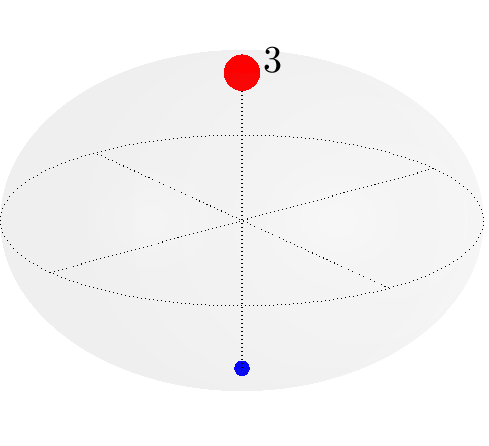
\includegraphics[width=0.3\textwidth]
            {gfx/ch-groundStateSymmetries/FM-1-Majorana.pdf}};
        \node at (9, 0){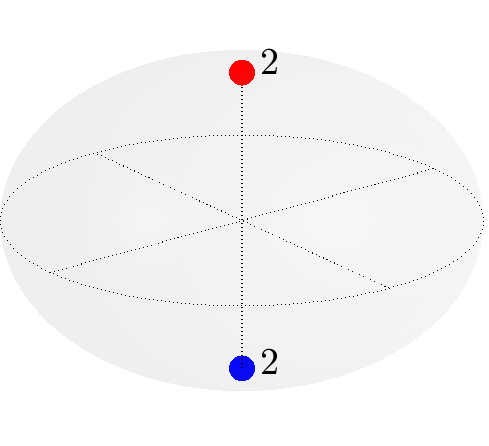
\includegraphics[width=0.3\textwidth]
            {gfx/ch-groundStateSymmetries/UN-Majorana.pdf}};
        \node at (11.8, -2.5) {
            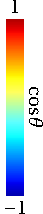
\includegraphics{gfx/colourbars/compiled_jet_majorana.pdf}};

        \node at (0, -2) {(a)};
        \node at (4.5, -2) {(b)};
        \node at (9, -2) {(c)};

        \node at (0, 2) {\(\zeta={(1, 0, 0, 0, 0)}^T\)};
        \node at (4.5, 2) {\(\zeta={(0, 1, 0, 0, 0)}^T\)};
        \node at (9, 2) {\(\zeta={(0, 0, 1, 0, 0)}^T\)};

        % Second row
        \node at (0, -5){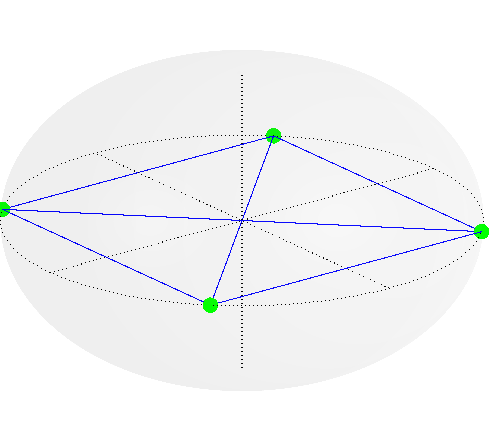
\includegraphics[width=0.3\textwidth]
            {gfx/ch-groundStateSymmetries/BN-Majorana.pdf}};
        \node at (4.5, -5){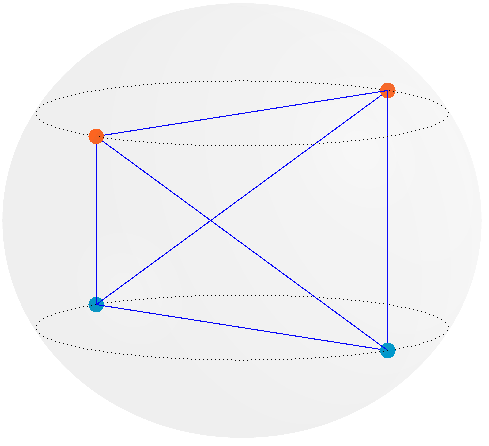
\includegraphics[width=0.265\textwidth]
            {gfx/ch-groundStateSymmetries/C1-Majorana.pdf}};
        \node at (9, -5){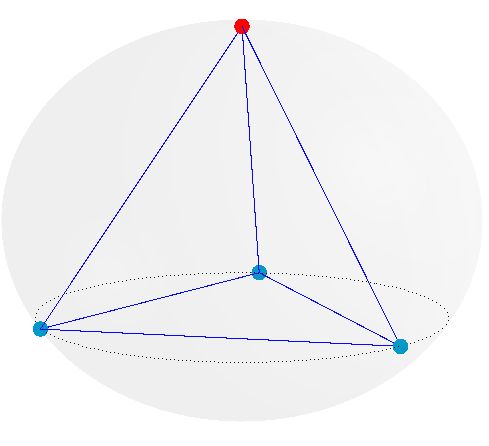
\includegraphics[width=0.275\textwidth]
            {gfx/ch-groundStateSymmetries/C2-Majorana.pdf}};

        \node at (0, -7) {(d)};
        \node at (4.5, -7) {(e)};
        \node at (9, -7) {(f)};

        \node at (0, -3) {\(\zeta={(1, 0, 0, 0, 1)}^T/\sqrt{2}\)};
        \node at (4.5, -3) {\(\zeta={(1, 0, i\sqrt{2}, 0, 1)}^T/2\)};
        \node at (9, -3) {\(\zeta={(\sqrt{1/3}, 0, 0, \sqrt{2/3}, 0)}^T\)};
    \end{tikzpicture}
    \caption[Majorana representation of spin-2 ground states]
    {\label{fig: spin-2-Majorana}Majorana representation of spin-2 ground
    states.
    As in the spin-1 case, the colour of the points represent \(\cos\theta =
    (1-|z|^2)/(1+|z|^2)\), whilst a number next to a point represents the root
    when the polynomial \(P_\psi^1(z)\) has an \(n\)-multiple root.
    (a): FM-2 state with \(\zeta={(1, 0, 0, 0, 0)}^T\).
    (b): FM-1 state with \(\zeta={(0, 1, 0, 0, 0)}^T\).
    (c): UN state with \(\zeta={(0, 0, 1, 0, 0)}^T\).
    (d): BN state with \(\zeta={(1, 0, 0, 0, 1)}^T/\sqrt{2}\).
    (e): Three-component cyclic state with
    \(\zeta={(1, 0, i\sqrt{2}, 0, i)}^T/2\).
    (f): Two-component cyclic state with
    \(\zeta={(\sqrt{1/3}, 0, 0, \sqrt{2/3}, 0)}^T\).}
\end{figure}

\section{Topological defects in spin-1 BECs}
Due to their rich phase diagrams discussed in the previous sections, spinor BECs
give rise to multiple different types of topological defects.
Such defects range from vortices, both singular~\cite{Yip1999,Isoshima2002,
Mizushima2002, Sadler2006,Semenoff2007,Lovegrove2012,Lovegrove2016,
Borgh2016,Weiss2019,Xiao2021,Xiao2022}, fractional~\cite{Leonhardt2000,
Zhou2003,Ji2008,Seo2015,Semenoff2007,Kobayashi2009,Lovegrove2012,
Lovegrove2016,Borgh2016,Borgh2017,Xiao2021,Xiao2022}, and
nonsingular~\cite{Ohmi1998, Ho1998, Mizushima2002a,
Martikainen2002, Leanhardt2003, Mizushima2004, Choi2012, Choi2012a,
Lovegrove2014,Weiss2019}, to point defects such as monopoles~\cite{Stoof2001,
Savage2003,Ruostekoski2003, Pietila2009,Ray2014,Ray2015,Ollikainen2017,
Mithun2022}.

\subsection{Polar phase}
\subsection{Ferromagnetic phase}

\section{Topological defects in spin-2 BECs}
\section{Uniaxial nematic phase}
\section{Biaxial nematic phase}
\section{Cyclic phase}
\section{Ferromagnetic phase}

\section{Topological defects in spinor BECs}
\subsection{Spin-1}\label{sec: vortices-spin-1}
We start with the polar phase of a spin-1 condensate, with the representative
spinor defined as in Eq.~\eqref{eq: polar-representative-spinor}.
Unlike the scalar BEC, a singly quantised vortex in the polar phase does not
represent the lowest unit of circulation.
Instead, the polar phase allows for a vortex where the global phase only winds
by \(\pi \) about the vortex core.
This \(\pi \) rotation is then coupled with a \(\pi \) spin rotation to the
nematic director \(\hat{\vb{d}}\) to keep the order parameter single valued.

If we consider a vortex that is oriented along the \(z\)-axis and the nematic
director is oriented in the \((x, y)\)-plane, then such a vortex corresponds to
the choice of \(\tau=\alpha=\varphi/2 \) and \(\beta = \pi/2\) in
Eq.~\eqref{eq: polar-representative-spinor} to yield the wave function
\begin{equation}
    \psi^\mathrm{HQV} = \sqrt{\frac{n}{2}} \mqty(
    -1 \\
    0 \\
    e^{i\varphi}
    ),
    \label{eq: polar-HQV}
\end{equation}
where \(\varphi \) is the azimuthal angle about the vortex core.
Such a vortex is referred to as a half-quantum vortex (HQV) due to carrying
half the typical circulation of a scalar \(U(1)\) vortex.
Similar, but topologically distinct vortices arise in the A phase of
superfluid \( ^3\)He~\cite{Salomaa1985, Salomaa1987}.

In experiment, for the vortex constructed as in Eq.~\eqref{eq: polar-HQV}, the
vortex consists of density depletion along the core in the \(\psi_{-1}\)
component, where the phase winding is located.
This core is then filled with atoms of the \(\psi_1 \) component, which lifts
the core out of the polar phase and into the ferromagnetic phase.
Fig.~\ref{fig: spin-1-vortices}a shows the spherical harmonic representation of
the HQV\@.
\begin{figure}
    \centering
    \begin{tikzpicture}
        \node at (0, 0) {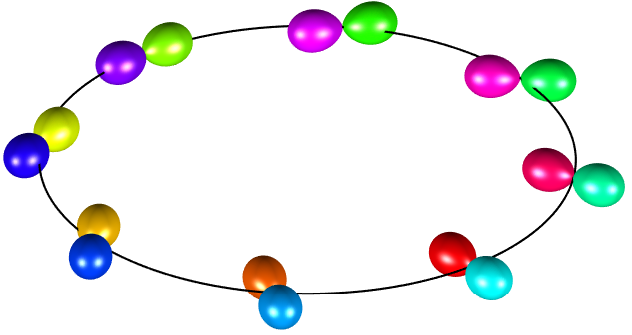
\includegraphics[width=0.45\textwidth]
            {gfx/ch-groundStateSymmetries/polar-HQV.pdf}};
        \node at (7.2, 0) {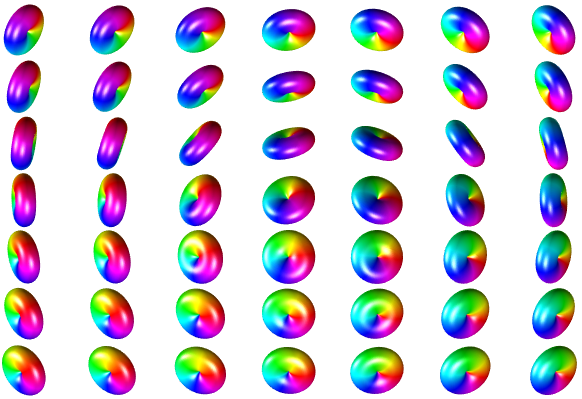
\includegraphics[width=0.45\textwidth]
            {gfx/ch-groundStateSymmetries/coreless.pdf}};
        \node at (-3.6, -0.2) {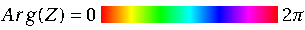
\includegraphics[angle=90]
            {gfx/colourbars/compiled_hsv.pdf}};

        % Labels
        \node at (0, -3) {(a)};
        \node at (7.2, -3) {(b)};
    \end{tikzpicture}
    \caption[Spherical harmonic representation of spin-1 vortices]
    {\label{fig: spin-1-vortices}Spherical harmonic representation of vortices
        in a spin-1 BEC\@.
        (a): Spin-1 polar HQV defined by Eq.~\eqref{eq: polar-HQV}.
        A complete circuit of the vortex results in a \(\pi \) spin rotation of
        the nematic director coupled with a \(\pi \) change to the condensate
        phase.
        (b): Ferromagnetic coreless vortex.
        The vortex takes on a characteristic fountain-like texture of the
        condensate spin vector.
    }
\end{figure}

The ferromagnetic phase has the unique property that circulation is not
quantised~\cite{Kawaguchi2012}.
This leads to both singular and non-singular defects present in this phase.
Here, we discuss a particular type of non-singular vortex called the coreless
vortex~\cite{Martikainen2002, Leanhardt2003}.

From Eq.~\eqref{eq: FM-representative-spinor}, a coreless vortex is constructed
using the choice of \(\tau-\gamma = \alpha= \varphi \) and having
\(\beta = \beta(\rho)\) be a function of the radial coordinate, \(\rho \):
\begin{equation}
    \psi^\mathrm{coreless} = \sqrt{n}\mqty(
    \cos^2\frac{\beta}{2} \\
    \frac{e^{i\varphi}}{\sqrt{2}}\sin\beta \\
    e^{2i\varphi}\sin^2\frac{\beta}{2}
    ).
\end{equation}
The single-valued condition of the wave function is satisfied by choosing
\(\beta \) such that \(\beta(r=0) = 0\) and \(\beta(r=r_0) = \pi \), where
\(r_0\) is the radius of the system.
This choice of \(\beta \) results in a vortex-free configuration at \(r=0\),
which then terminates on a doubly-quantised vortex at \(r=r_0\).
A spherical harmonic representation of the coreless vortex is shown in
Fig.~\ref{fig: spin-1-vortices}b, where the characteristic fountain-like
spin texture is apparent.

\subsection{Spin-2}\label{sec: vortices-spin-2}
Spin-2 BECs offer an even richer diagram of topological defects than their
spin-1 counterparts.
We start with the UN phase, as given by
Eq.~\eqref{eq: UN-representative-spinor}.
Unlike the spin-1 polar phase, the UN phase does not support fractional vortices
with mass circulation.
This is apparent from the spherical harmonic representation given in
Fig.~\ref{fig: spin-2-spherical-harmonics}c, where the \(\mathbb{Z}_2\) symmetry
about the \(C_2\) axis is not coupled to the condensate phase, \(\tau \).
This phase instead accommodates a spin vortex, i.e., a vortex which carries only
spin circulation.
Such a vortex is constructed from Eq.~\eqref{eq: UN-representative-spinor} with
the choice \(\tau=0, \alpha=-\varphi/2, \beta=\pi/2\):
\begin{equation}
    \psi^\mathrm{SV} = \frac{\sqrt{6n}}{4}\mqty(
    e^{i\varphi} \\
    0 \\
    -\sqrt{\frac{2}{3}} \\
    0 \\ e^{-i\varphi}
    ).
\end{equation}
The spherical harmonic representation of this vortex state is shown in
Fig.~\ref{fig: SV-HQV}a.
\begin{figure}
    \centering
    \begin{tikzpicture}
        \node at (0, 0) {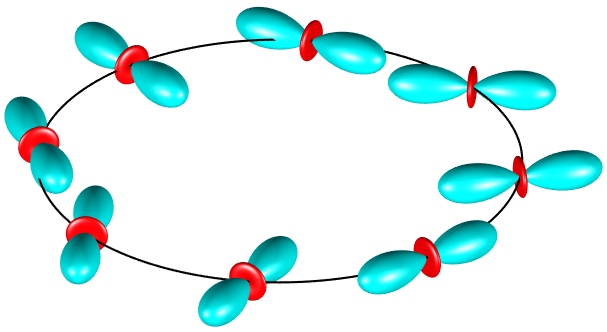
\includegraphics[width=0.45\textwidth]
            {gfx/ch-groundStateSymmetries/UN-spin-vortex.pdf}};
        \node at (7.3, 0) {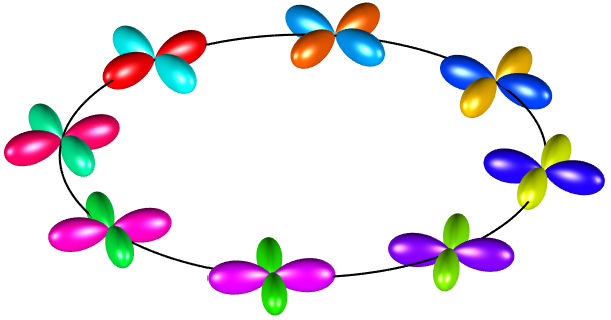
\includegraphics[width=0.45\textwidth]
            {gfx/ch-groundStateSymmetries/BN-HQV.pdf}};
        \node at (3.0, -2) {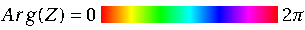
\includegraphics{gfx/colourbars/compiled_hsv.pdf}};

        % Labels
        \node at (-0.8, -2.2) {(a)};
        \node at (7.2, -2.2) {(b)};
    \end{tikzpicture}
    \caption[Spherical harmonic representation of spin-2 vortices]
    {\label{fig: SV-HQV}Spherical harmonic representation of select vortices in the spin-2
        nematic phases.
        (a): A spin vortex in the UN phase. A complete circuit of the vortex
        results in a \(\pi \) winding of the condensate spin vector, with no
        change to the condensate phase.
        (b): One type of half-quantum vortex in the BN phase.
        The condensate phase winds by \(\pi \) about the vortex core which is
        coupled to a \(\pi / 2\) spin rotation.}
\end{figure}
As the core of the vortex is traversed, the spin vector winds by \(\pi \) about
the axis perpendicular to the nematic director, \(\hat{\vb{d}}\).

The BN phase is the simplest order parameter that supports non-abelian defects,
i.e., defects whose topological charges do not commute~\cite{Mermin1979}.
One of the simplest defects in this phase is the half-quantum vortex.
However, this is topologically distinct from that of the spin-1 polar case.
Such a vortex can be constructed from Eq.~\eqref{eq: BN-representative-spinor}
using the choice \(\tau=2\alpha=\varphi/2\) and \(\beta=\gamma=0\):
\begin{equation}
    \psi^\mathrm{1/2-1/4} = \sqrt{\frac{n}{2}}\mqty(
    1 \\
    0 \\
    0 \\
    0 \\
    e^{i\varphi}
    ).
\end{equation}
The spherical harmonic representation of this vortex is shown in
Fig.~\ref{fig: SV-HQV}b.
It is the clear the condensate phase winds by \(\pi \) about the vortex core,
which is also coupled to a \(\pi / 2\) spin rotation.
This configuration is sometimes denoted a \(1/2-1/4\) vortex, where the \(1/2\)
and \(1/4\) denote the phase and spin rotation angles, respectively.

This is not the only type of HQV that the BN phase supports.
For example, there exists a pure spin vortex (\(0 - 1/2\) vortex) and a HQV
that is also coupled to a \(\pi \) spin rotation
(\(1/2-1/2\) vortex)~\cite{Kawaguchi2012}.

Finally, the cyclic phase also allows for fractional vortices.
However, the circulation in this phase is quantised in units of \(\kappa / 3\),
leading to \(1/3\) and \(2/3\) vortices.
These vortices are constructed by applying a condensate phase and general spin
rotation to Eq.~\eqref{eq: C-2-spinor}.
A \(1/3\) vortex is constructed from the choice
\(\tau = -\alpha = \varphi/3 \) with \(\gamma = 0\).
Similarly, a \(2/3\) vortex is constructed by choosing \(\tau = 2\varphi/3\),
\(\alpha = \varphi/3\) and \(\gamma=0\).
The result is a phase winding in the \(\psi_2\) and \(\psi_{-1}\) components
for the \(1/3\) and \(2/3\) vortices, respectively:
\begin{equation}
    \psi^{1/3} = \sqrt{\frac{n}{3}}\mqty(e^{i\varphi} \\ 0 \\ 0 \\ \sqrt{2}\\0),
    \qquad
    \psi^{2/3} = \sqrt{\frac{n}{3}}\mqty(1 \\ 0 \\ 0 \\\sqrt{2}e^{i\varphi}\\0).
\end{equation}
Spherical harmonic representations are plotted in
Fig.~\ref{fig: cyclic-fractional-spherical}.
\begin{figure}
    \centering
    \begin{tikzpicture}
        \node at (0, 0) {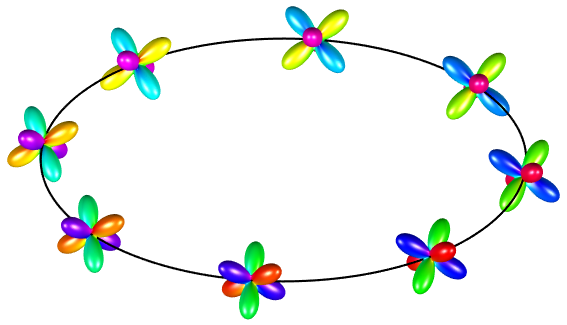
\includegraphics[width=0.45\textwidth]
            {gfx/ch-groundStateSymmetries/one-third-vortex.pdf}};
        \node at (7.3, 0) {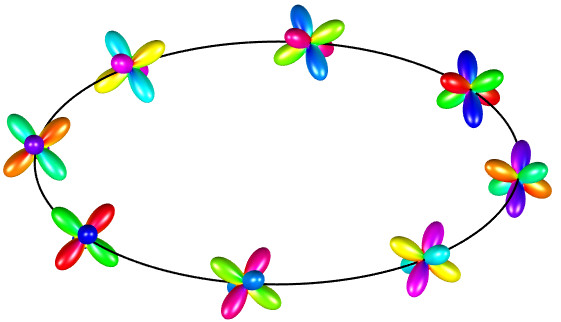
\includegraphics[width=0.45\textwidth]
            {gfx/ch-groundStateSymmetries/two-third-vortex.pdf}};
        \node at (3, -2) {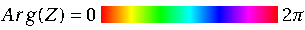
\includegraphics{gfx/colourbars/compiled_hsv.pdf}};

        \node at (0, -2.2) {(a)};
        \node at (7.2, -2.2) {(b)};
    \end{tikzpicture}
    \caption[Spherical harmonic representation of cyclic fractional vortices]
    {\label{fig: cyclic-fractional-spherical}Spherical harmonic
        representations of cyclic fractional vortices.
        (a): The \(\frac{1}{3}\) vortex. A complete circuit reveals a \(2\pi/3\)
        winding of the condensate phase, coupled with a \(\pi/2\) spin rotation.
        (b): The \(\frac{2}{3}\) vortex. Similarly, a complete circuit of the
        vortex results in a \(4\pi/3\) winding of the condensate phase, again
        coupled to a \(\pi/2\) spin rotation.}
\end{figure}


\part{Numerical studies of spinor and pseudospinor condensates}
\chapter{Relaxation dynamics in a two-component system}

\section{Introduction}
Since the realization of superfluidity, quantum turbulence (QT) has been studied
in systems ranging from superfluid liquid
Helium~\cite{Barenghi2014, Walmsley2014} to quasi-particle
condensates in solid-state systems~\cite{Kreil2018}.
Due to their unprecedented experimental accessibility, QT in Bose-Einstein
condensates (BECs) in dilute, ultra-cold atomic gases have attracted considerable
theoretical~\cite{Kobayashi2007,Numasato2010, Reeves2013,
Billam2014,Simula2014,Baggaley2018} and
experimental~\cite{Henn2009,Kwon2014,Seo2017,Navon2019,Gauthier2019,
Johnstone2019} interest in both 2D and 3D configurations.
In a scalar BEC, the QT state is made up of a large number of vortices with
quantised circulation.
The collective behaviour of the vortices plays a key role
in the hydrodynamics, recovering features of classical turbulence that can
exhibit the characteristic Kolmogorov power-law spectrum~\cite{Kobayashi2005}.


In contrast to the scalar superfluids, multi-component and spinor BECs are
described by multi-component order parameters and allow for a wider range of
topological defects, which give rise to novel dynamics~\cite{Kasamatsu2016,
Weiss2019,Kobayashi2009,Kasamatsu2005}.
Consequently, there has been increasing interest in the properties of QT and
non-equilibrium dynamics in such
systems~\cite{Salman2009, Schmied2019, Karl2013, Prufer2018, Hofmann2014}.
The simplest non-scalar topological excitation appears in a two-component BEC,
described by two complex fields, as the appearance of a phase singularity in
only one component. 
When the atomic mass and mean density of the components are equal, such vortices
are often referred to as half-quantum vortices (HQVs), due to their similarities
with vortices carrying half a quantum of superfluid circulation in superfluid
\(^3\)He~\cite{Autti2016} and spin-1 BECs~\cite{Leonhardt2000,Seo2015}.
The study of QT in BECs can be separated into two distinct categories: 1.\
forced turbulence where a statistically stationary state is established;
2.\ decaying turbulence where a non-equilibrium initial condition, typically
involving vortices, relaxes towards equilibrium. 

As we have seen \textcolor{red}{IN RELEVANT PART}, the two-component BEC can be 
treated as a pseudospin-1/2 system. 
This new system gives rise to novel defects such as a half-quantum vortex 
otherwise unseen in a scalar condensate. 
In this chapter, we investigate the relaxation dynamics of half-quantum vortices 
(HQVs) in a two-dimensional, two-component condensate. 
Our interest is in studying the scaling laws that govern the decay rate of the 
vortices, and consequently the growth of the length scales associated with 
domains in the system, whilst varying the ratio of inter- to intra-species 
interactions. 
We study these scales by starting from an initially turbulent state containing
HQVs and subsequently letting the system relax in time.
Upon relaxation, vortices will annihilate leading to domain growth within 
the system.
To extract the appropriate length scales of these domains, we construct 
correlation functions, originally defined for an antiferromagnetic spin-1 
system~\cite{Symes2017}, which then allow us to extract relevant length scales
associated with spin and mass order.
By investigating these length scales temporally, we reveal interesting, 
novel dynamics occurring at early times for a sufficiently high ratio of 
inter- to intra-species interactions. 
This result is then confirmed by considering the total vortex number of the 
system. 
Furthermore, we contrast our observations for this system with similar
simulations that have been performed for scalar BECs and reported
in~\cite{Schole2012, Nowak2012, Karl2017}.
Finally, we discuss how our observations of anomalous vortex decay can be
explained by relating to previous work~\cite{Eto2011, Kasamatsu2016}.


\section{Two-component BEC as a pseudospinor}

\subsection{Easy-plane polar phase}\label{subsec:easy-plane-polar-phase}
The two-component BEC can be regarded as a `pseudospin-1/2' system as it can be
mapped directly to a certain configuration of the spin-1 condensate.
Recall that the spin-1 condensate with polar interactions \((c_2 > 0)\) supports a
polar ground state with \(|\vb{F}|=0\).
This state can be categorized in two different ways depending on the orientation
of the nematic director.
The first consists of the nematic director being aligned with the \( z \)-axis,
which is referred to as the easy-axis polar (EAP) phase.
This phase is stable for \( p=0 \) and \( q>0 \)
\textcolor{red}{See relevant section?}.
The second case consists of the director being in the \( xy \)-plane, which is
referred to as the easy-plane polar (EPP) phase.
This phase is stable for \( p=0 \) and \( q < 0 \).
The representative wavefunction for the EPP phase can be written as
\begin{equation}
    \psi_\mathrm{EPP} = \frac{1}{\sqrt{2}}\begin{pmatrix}
        1 \\ 0 \\ 1
    \end{pmatrix}.
    \label{eq:EPP_wavefunction}
\end{equation}
Since the middle component is empty, we can map this spinor directly onto a
two-component system.

\subsection{Mapping the EPP phase onto a two-component system}\label{subsec:mapping-the-epp-phase-onto-a-two-component-system}
To begin the mapping procedure, we first construct the time-independent
GPEs for the spin-1 system with a wavefunction that assumes an empty middle
component:
\begin{equation}
    \begin{aligned}
        \left[-\frac{\hbar^2\nabla^2}{2M}
        + (c_0 + c_2)|\psi_1|^2 + (c_0 - c_2)|\psi_{-1}|^2 
        + q - \mu\right]\psi_1 &= 0, \\
        \left[-\frac{\hbar^2\nabla^2}{2M}
        + (c_0 + c_2)|\psi_{-1}|^2 + (c_0 - c_2)|\psi_1|^2 
        + q - \mu\right]\psi_{-1} &= 0,
    \end{aligned}
    \label{eq:EPP-time-independent-GPEs}
\end{equation}
where \( \mu \) is the chemical potential of the system, and we have taken
\( p=0 \).

Similarly, the time-independent GPEs for the two-component system are
\begin{equation}
    \begin{aligned}
        \left(-\frac{\hbar^2\nabla^2}{2m_1} + g_1|\psi_1|^2
        +g_{12}|\psi_2|^2 - \mu_1\right)\psi_1 &= 0, \\
        \left(-\frac{\hbar^2\nabla^2}{2m_2} + g_2|\psi_2|^2
        +g_{12}|\psi_1|^2 - \mu_2\right)\psi_2 &= 0.
    \end{aligned}
    \label{eq:two-comp-time-independent-gpes}
\end{equation}
Using these time-independent equations, we can map the two-component system
to that of the spin-1 by comparing the coefficients with
Eq.~\eqref{eq:EPP-time-independent-GPEs}.
By doing this we find
\begin{equation}
    g_1=g_2=c_0+c_2, \enskip g_{12} = c_0-c_2, \enskip \mu_1=\mu_2=\tilde{\mu}, 
    \enskip m_1=m_2=M,
\end{equation}
where \( \tilde{\mu} = \mu - q \).
This directly relates the two-component BEC to the EPP phase of a spin-1
condensate.
Note that this mapping only holds when the interspecies interactions, chemical
potentials and masses of the atomic species in the two-component BEC are equal.
\textcolor{red}{Links to papers that discuss this particular type of
two-component BEC?}


\section{Half-quantum vortices in spin-1/2}
The pseudospinor nature of the two-component system allows for a novel vortex
structure otherwise unseen in scalar BECs.
To construct such a vortex, we start by defining the pseudospin-1/2
wavefunction:
\begin{equation}
    \mqty(\psi_1 \\ \psi_2) = 
    \mqty(|\psi_1|e^{i\theta_1} \\ |\psi_2|e^{i\theta_2}) = 
    e^{i\Theta}\mqty(|\psi_1|e^{i\Phi} \\ |\psi_2|e^{-i\Phi}),
    \label{eq:pseudospin-1/2-wavefunction}  
\end{equation}
where \( \theta_j=\mathrm{Arg}(\psi_j) \) for \( j=1,2 \) and
\begin{equation}
    \Theta = \frac{\theta_1 + \theta_2}{2}, \enskip 
    \Phi = \frac{\theta_1 - \theta_2}{2}.
    \label{eq:Theta-Phi}
\end{equation}
Gradients in \( \Theta \) are associated with a total, superfluid mass current
whereas gradients in \( \Phi \) are associated with pseudospin currents.
\textcolor{red}{Do I want to elaborate on this further? Potentially by looking
at actual expressions for mass and pseudospin current in two-component BECs.}
Now consider a vortex state which consists of a phase singularity in the
\(\psi_1 \) component such that about the singularity \( \theta_1 \) winds by
\( 2\pi \) and \( \theta_2 \) remains unchanged, i.e.\ it is a smooth phase
field.
Such a state can be written as
\begin{equation}
    \twovec{\psi_1}{\psi_2} 
    = \twovec{|\psi_1|e^{i\varphi}}{|\psi_2|}
    = e^{\varphi/2}\twovec{|\psi_1|e^{i\varphi/2}}{|\psi_2|e^{-i\varphi/2}},
\end{equation}
where \( \varphi \) is the azimuthal angle around the vortex core.
By comparing the above to Eq.~\eqref{eq:pseudospin-1/2-wavefunction}, we have
\( \Theta=\Phi=\varphi/2 \).
Using the fact the velocity is related to phase \(\vb{v}=\hbar/m\grad\Theta \),
the circulation is then given by
\begin{equation}
    \oint_C\vb{v}\cdot d\vb{\ell} = q\frac{\kappa}{2},
\end{equation}
where \( q \) denotes the charge of the vortex and \(\kappa=\hbar/m\) is the
quantum of circulation.
Traversing a point about the vortex shows the circulation is quantised in units
of \(\kappa/2\), half the usual circulation of \( U(1) \) vortices in scalar
BECs [REFs?].
Since this vortex carries half the circulation of a \( U(1) \) vortex, such a
vortex state is referred to as a half-quantum vortex\footnote{This vortex is 
topologically distinct from HQVs that arise in the A and polar phases of
superfluid \(^3\)He~\cite{Autti2016} and the polar phase of spin-1
BECs~\cite{Leonhardt2000, Seo2015}.}.

\section{Half-quantum vortex relaxation dynamics}
To begin studying the relaxation dynamics of HQVs in a turbulent system, we
numerically solve the two-component Gross-Pitaevskii equations in dimensionless
form
(\textcolor{red}{see Appendix for details of dimensionless form}):
\begin{equation}
    \begin{aligned}
        i\frac{\partial \psi_1}{\partial t} &= (-\nabla^2 + g|\psi_1|^2
        + \gamma|\psi_2|^2)\psi_1, \\
        i\frac{\partial \psi_2}{\partial t} &= (-\nabla^2 + g|\psi_2|^2
        + \gamma|\psi_1|^2)\psi_2.
    \end{aligned}
    \label{eq:dimensionless-two-comp-GPEs}
\end{equation}
where we have assumed each component has the same atomic mass and inter-species
interaction strength.
The key parameter is the ratio of inter- to intra-species interaction
\begin{equation}
    \gamma = \frac{g_{12}}{g}.
\end{equation}
We consider the case \(0 < \gamma < 1\) with all interactions repulsive such that
the condensate is stable against the separation of the components.

The inter- and intra-component interactions give rise to two important length
scales within the system.
These are, respectively, associated with variations in the total superfluid
density and the difference in density between the components.
The density and spin healing lengths are then defined as~\cite{Eto2011}
\begin{equation}
    \xi_d = \frac{\hbar}{\sqrt{2mgn_0}}, \qquad 
    \xi_s = \xi_d \sqrt{\frac{1 + \gamma}{1 - \gamma}},
    \label{eq:healing-lengths}
\end{equation}
where \(n_0\) is the background number density of each component in a uniform
system.
The size of the HQV core can be understood from the energetic hierarchy of
these healing lengths.
Since an HQV consists of a phase singularity in one component and not the other,
the core is free to fill with the atoms of the other component.
This corresponds to spatial variations in the \( z \)-component of the
pseudospin, the size of which is set by the spin healing length, \(\xi_s\).
The vortex core can expand when \(\xi_s \lesssim \xi_d\), which lowers
the total energy.
We see from Eq.~\eqref{eq:healing-lengths} that \(\gamma \) directly determines
the core sizes within our systems.
Similar energetic hierarchies exist in spinor BECs, which can facilitate
deformations of vortex cores such as the splitting of singly quantized vortices
into fractional vortices [REFS].

\subsection{Numerical setup}\label{sec:numerical-setup}
We solve Eq.~\eqref{eq:dimensionless-two-comp-GPEs} on a periodic domain with 
\(N_s^2=1024^2\) grid points which has dimensionless area \(L^2=N_s^2\) with
side length \(L=N_s\).
We take \(N=3.2\times10^9\) atoms per component and fix dimensionless
\(g=L^2/4N\).
The dimensionless density healing length is then fixed at
\(\xi_d=N_s/\sqrt{gN}=2\) in our system.
We wish to explore the effect of the inter-component interaction by varying
\(\gamma \) within the range \(0 < \gamma < 1\).

The initial state is constructed as follows.
We wish to construct \(48^2\) vortices in each component.
To do this we start with a grid of vortex positions such that the 
\(i\)-th vortex is to be imprinted at position \((x_i, y_i)\).
We repeat the same procedure for the other component.
However, to avoid overlapping vortex positions, we offset this grid in both
\(x\) and \(y\) whilst preserving the grid structure.
To facilitate a random distribution of vortices and subsequently turbulent
dynamics, we then displace each position by some small amount 
\((x_i, y_i) \rightarrow (x_i \delta + x_i, y_i + \delta y_i)\), where 
\(\delta x_i, \delta y_i < 3\xi_d\).
The vortices are then constructed as an alternating \( 2\pi \) winding of the
component phase about each vortex position using the method described
in~\cite{Billam2014}.
We imprint the vortices using a short imaginary time propagation of
Eq.~\eqref{eq:dimensionless-two-comp-GPEs} whilst keeping the phase profile
fixed to not alter the positions of the vortices.
This results in an initially turbulent system of HQVs.
The HQV cores correspond to a density depletion in one component at the position
of the phase singularity with a corresponding density peak at the same position
in the other component (see Fig.~\ref{fig:initial-vortex-state}).
\begin{figure}
    \centering
    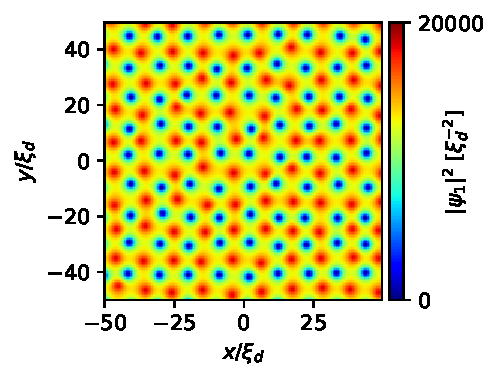
\includegraphics{gfx/ch-twoCompDynamics/init_state.pdf}
    \caption{Density of \(\psi_1 \) component in a \(100\xi_d\times100\xi_d\)
    subregion of the initial state after imaginary time propagation.
    We see the HQVs in this component by the density depletion.
    The density peaks correspond to the location of HQV cores in the other
    component, which have been filled by atoms in this
    component.\label{fig:initial-vortex-state}}
\end{figure}
Previous work has shown that clustering of vortices can lead to anomalously
slow coarsening dynamics~\cite{Karl2017} and thus constructing the initial
state this way ensures that there is no clustering of like-signed vortices.
From this initial state, the system evolves according to
Eq.~\eqref{eq:dimensionless-two-comp-GPEs}.
Two HQVs in the same component with opposite winding can annihilate, leading to
a decay of the total vortex number within the system.

\subsection{Interaction dependence of HQV core size}
We first investigate how \(\gamma \) affects the HQVs within our systems.
\begin{figure}
    \centering
    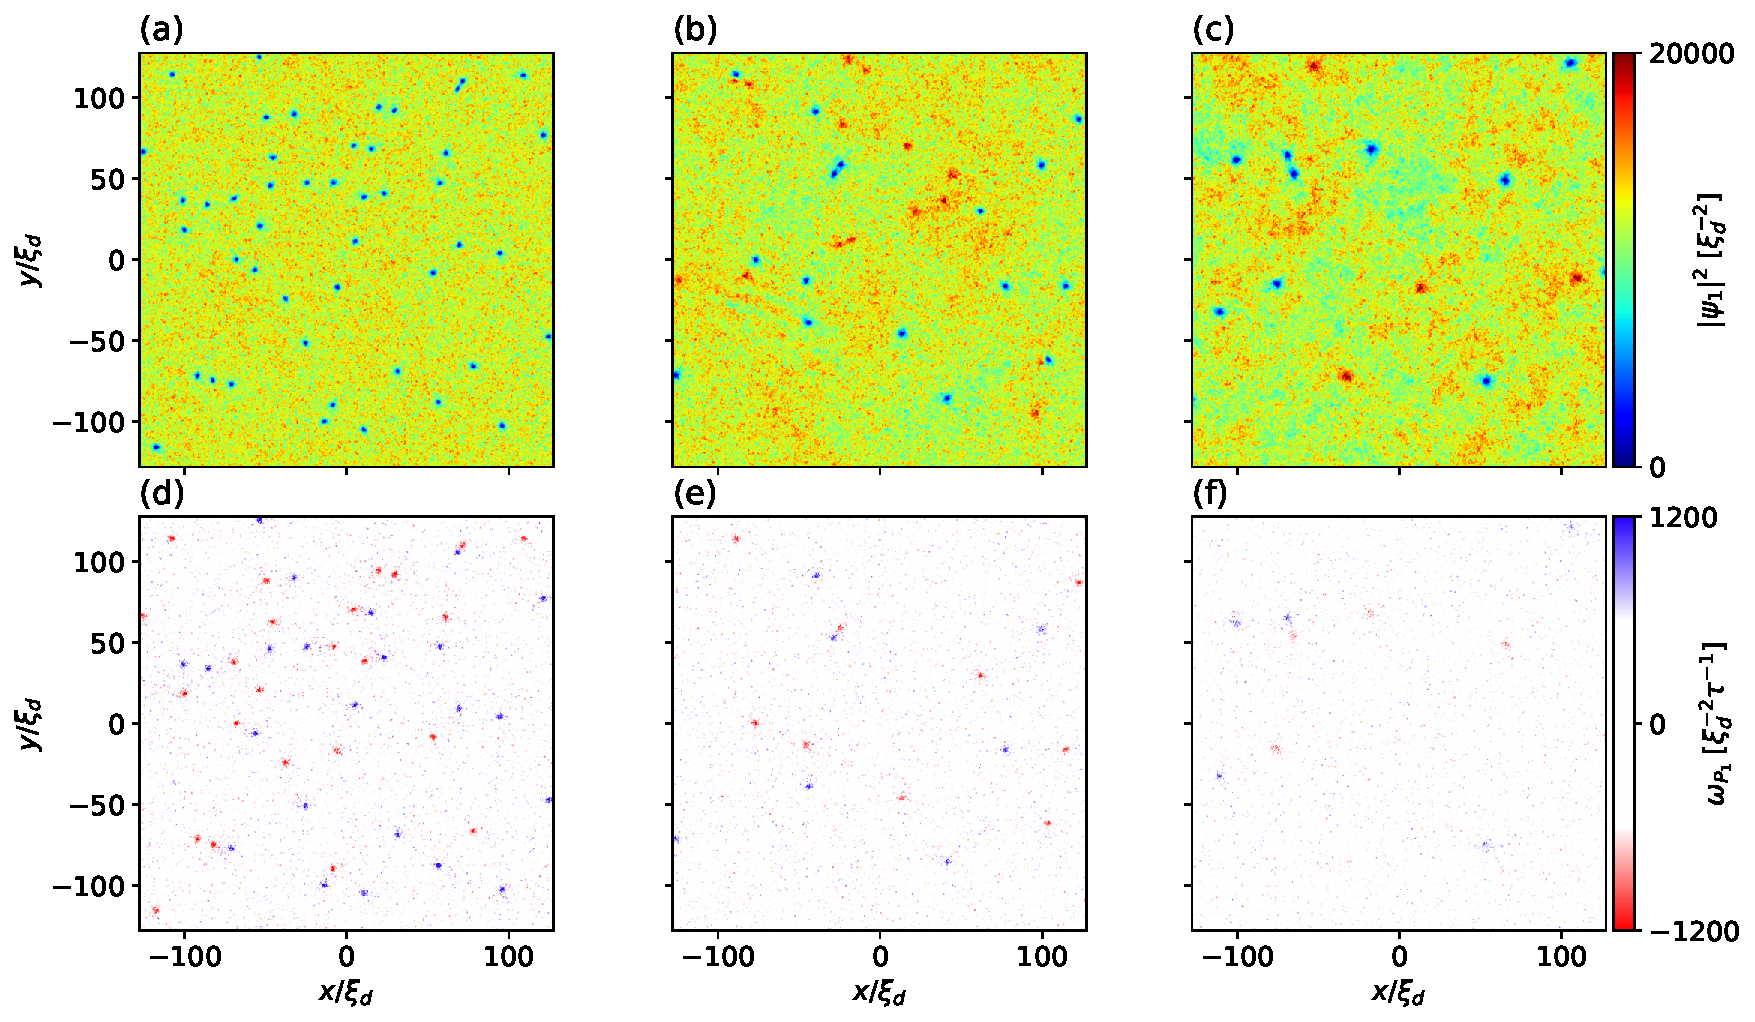
\includegraphics[width=\textwidth]{gfx/ch-twoCompDynamics/densVort.pdf}
    \caption{Density (a)- (c) and pseudo-vorticity (d)- (f) of the \(\psi_1 \)
    component in a \(256\xi_d \times 256\xi_d\) subregion at a time 
    \(t/\tau=2.5\times 10^4\xi_d^2\) for \(\gamma=0.1\) (left),
    \(\gamma=0.6\) (middle), and \(\gamma=0.8\) (right).
    The density depletions correspond to HQVs in this component.
    For \(\gamma \gtrsim 0.6\), density peaks reveal the locations of HQVs with
    the phase singularity in the other component where the cores have filled
    with atoms in this component.
    Vortices with positive (blue) and negative (red) circulation are
    identifiable in the pseudo-vorticity field.\label{fig:density-pseudo-vort}}
\end{figure}
Fig.~\ref{fig:density-pseudo-vort} shows the density field of the \(\psi_1 \)
component for \(\gamma = 0.1, 0.6, 0.8\).
One sees that as \(\gamma \) increases, the core size (i.e., the radial size of
the density depletion) also increases.
From Eq.~\eqref{eq:healing-lengths} we see that the size of the HQV core is
dependent on \(\gamma \), where \(\xi_s \rightarrow \xi_d\) as
\(\gamma \rightarrow 0\).
The healing lengths can explain why, for \(\gamma \geq 0.6\), bright density
peaks also appear within the \(\psi_1 \) field.
For small \(\gamma \), the density and spin healing lengths become comparable,
\(\xi_d \sim \xi_s\).
However, an increasing \(\gamma \) implies a larger spin healing length.
Consequently, atoms of the other component will fill the vortex core as the
resulting lowering of the kinetic energy offsets the cost of interaction energy.
This results in the expansion of the vortex cores to the size of the spin
healing length.
Hence, bright density peaks in Fig.~\ref{fig:density-pseudo-vort} correspond to
atoms in the \(\psi_1 \) component that has filled the core of an HQV in the
\(\psi_2\) component. \par
We can accurately track the positions of the HQVs in the system through
the pseudo-vorticity [REFS]
\begin{equation}
    \omega_\mathrm{p_j} = \frac{1}{2}\nabla \times {(n\vb{v})}_j,
\end{equation}
where
\begin{equation}
    {(n\vb{v})}_j = -i\left[\psi_j^*(\nabla\psi_j) - (\nabla_j^*)\psi_j\right]
\end{equation}
is the mass current of component \(j=1, 2\).
The pseudo-vorticity has the unique property of remaining regular and non-zero
within the vortex cores. On length scales greater than the spin healing length
away from a vortex core, the pseudo-vorticity quickly relaxes to zero as seen
in Fig.~\ref{fig:density-pseudo-vort} (d)- (f).
The sign of the pseudo-vorticity also determines the charge of the vortex.

\subsection{Investigating the kinetic energy spectrum}
A useful property to investigate in turbulent systems is the kinetic energy
spectrum [REFS?].
This spectrum provides useful insights into the spatial aspects of the
relaxation dynamics.
We start with the kinetic energy of the two-component system which is written
in terms of the density \(n_j\) and velocity \(\vb{v}_j\) of the \(j\)-th
component (\( j=1,2 \)) as
\begin{equation}
    E_\mathrm{kin} = \int d^2\vb{x} (|\nabla\sqrt{n_1}|^2 
    + |\nabla\sqrt{n_2}|^2)
    + \frac{1}{4}\int d^2\vb{x} (|\sqrt{n_1}\vb{v}_1|^2 
    + |\sqrt{n_2}\vb{v}_2|^2).
\end{equation}
The kinetic energy can be further decomposed into quantum pressure
(\( E^q\)) and a classical velocity (\(E^v\)) contributions:
\begin{equation}
    E^v = \frac{1}{4}\int d^2\vb{x} (|\sqrt{n_1}\vb{v}_1|^2 
    + |\sqrt{n_2}\vb{v}_2|^2),
\end{equation}
\begin{equation}
    E^q = \int d^2\vb{x} (|\nabla\sqrt{n_1}|^2 
    + |\nabla\sqrt{n_2}|^2).
\end{equation}

To extract energy spectra from these contributions, we define the generalized
velocities for the incompressible (i), compressible (c), and quantum pressure
(q) parts as
\begin{equation}
    \begin{aligned}
        \vb{w}^{i, c} &= \sqrt{n_1}\vb{v}_1^{i, c} + \sqrt{n_1}\vb{v}_1^{i, c}
        \\
        \vb{w}^q &= 2 (\nabla \sqrt{n_1} + \nabla \sqrt{n_2}).
    \end{aligned}
\end{equation}
Here, the incompressible and compressible parts of the velocity field are
extracted from a Helmholtz decomposition [REF] which splits the velocity into a 
divergence-free incompressible part, \(\nabla \cdot \vb{v}^i = 0\), and an 
irrotational, compressible part, \(\nabla \times \vb{v}^c=\vb{0}\).
Hence, in Fourier space, the kinetic energy spectrum can be calculated by
taking the Fourier transform of the generalized velocities and integrating over
the \(k\)-space angle as
\begin{equation}
    E^\delta(k) = \frac{1}{4} \int_{0}^{2\pi} d\Omega_k
    |\tilde{\vb{w}}^\delta(\vb{k})|^2
    \qquad (\delta = i, c, q),
\end{equation}
for wave number \(k=|\vb{k}|\).
The total kinetic energy is then given by the sum of each contribution,
integrated over all \(k\)
\begin{equation}
    E_\mathrm{kin} = \sum_\delta \int dk E^\delta (k) \qquad (\delta = i, c, q).
\end{equation}
The occupation numbers of each contribution are extracted as
\begin{equation}
    n^\delta(k) = k^{-2}E^\delta(k) \qquad (\delta = i, c, q).
\end{equation}
Finally, the total occupation number of the system is given as
\begin{equation}
    n(k) = \int_{0}^{2\pi} d\Omega_k \psi_1^*(k)\psi_1(k) 
    + \psi_2^*(k)\psi_2(k).
\end{equation}

\begin{figure}[t!]
    \centering
    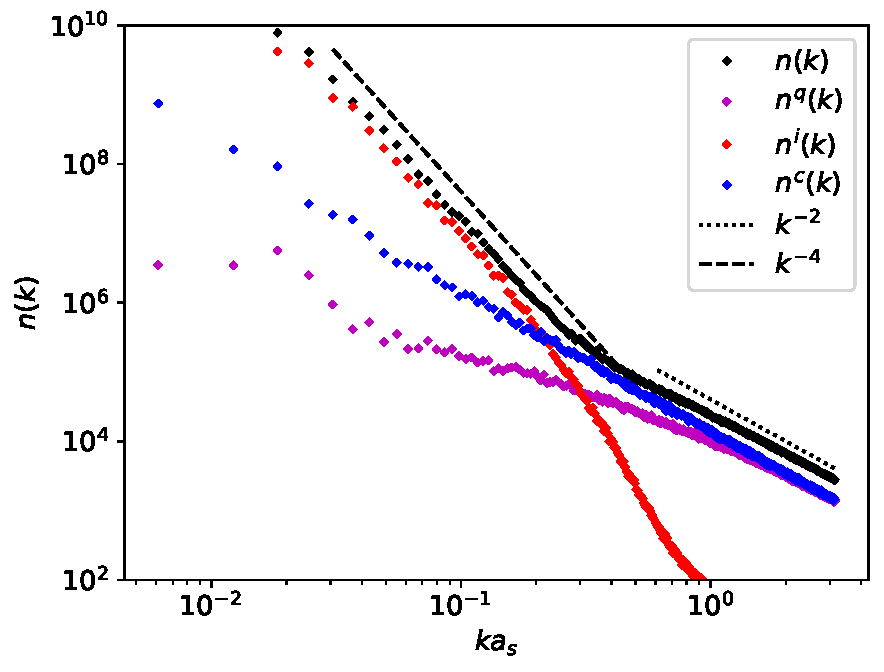
\includegraphics[scale=0.75]{gfx/ch-twoCompDynamics/spectra.pdf}
    \caption{Occupation numbers for the quantum pressure (purple diamonds),
    incompressible (red diamonds), and compressible (blue diamonds)
    contributions for \(\gamma=0.6\).
    The total occupation number (black diamonds) is obtained from the sum of
    each contribution.
    The total occupation number has two distinct scalings: a \(k^{-2}\) 
    (dotted line) in the ultra-violet region, and a \(k^{-4}\) scaling
    (dashed line) in the infrared.\label{fig:kinetic-energy-spectra}}
\end{figure}
We plot the occupation number for each energy contribution, as well as total
occupation number, at a late time for \(\gamma=0.6\) in
Fig.~\ref{fig:kinetic-energy-spectra}.
The total occupation number exhibits two different scalings: A \(k^{-4}\) in the
ultraviolet (UV), and \(k^{-2}\) in the infrared (IR). 
The same scalings have been found in some 2D, turbulent, scalar BEC systems
containing scalar vortices [REFS].
The decomposition of the kinetic energy into its respective contributions
allows us to see that the incompressible contribution dominates the spectrum
in the IR region, and is therefore responsible for the transition to the
\(k^{-4}\) scaling.
This incompressible contribution is directly associated with the vortices in
the system. \textcolor{red}{Elaborate? Why exactly?}
Similarly, we see it is both the compressible and quantum pressure contributions
that dominate in the UV region, facilitating the transition to the \(k^{-2}\)
scaling.
This \(k^{-2}\) scaling is characteristic of weak-wave turbulence [REFS].

This scaling of the kinetic energy was observed throughout all values of
\(\gamma \) tested, indicating that it is quantitatively insensitive to variations
in \(\gamma \).
The investigation into the kinetic energy spectrum reveals that \(\gamma \) has
negligible effects on the spatial aspects of the relaxation dynamics, and shows
quantitatively similar behaviour to some turbulent scalar BEC systems
containing scalar vortices.

\subsection{Spin spectra?}

\subsection{Temporal aspects of decay}
To measure the temporal aspect of the relaxation dynamics, we wish to
construct correlation functions.
Since our pseudo-spinor order parameter is composed of a mass part and a spin
part (c.f. Eq.~\eqref{eq:Theta-Phi}), it is natural to then construct both a
mass and spin correlation function.\par
To begin, we need to identify appropriate quantities that serve as order
parameters for our system.
By taking motivation from the EPP phase in spinor BECs, one such quantity is
the planar tensor~\cite{Symes2017}
\begin{equation}
    \mathsf{Q} = \mqty(Q_{xx} & Q_{xy} \\ Q_{xy} & -Q_{xx}),
\end{equation}
where \(Q_{xx} = \mathrm{Re}(\psi_1^*\psi_2)\) and
\(Q_{xx} = \mathrm{Im}(\psi_1^*\psi_2)\), showing this quantity depends on the
relative phase coherence of the two components.
The eigenvalues of \(\mathsf{Q}\) are given by
\{ \(-\frac{1}{2}|\alpha|, \frac{1}{2}|\alpha|\) \}, where
\(\alpha=-2\psi_1\psi_2\).
If we consider the general wavefunction defined in
Eq.~\eqref{eq:pseudospin-1/2-wavefunction}, then evaluating \(\mathsf{Q}\) and
\(\alpha \) gives
\begin{equation}
    Q_{xx} = |\psi_1||\psi_2|\cos({2\Phi}), \qquad 
    Q_{xy} = -|\psi_1||\psi_2|\sin({2\Phi}),
\end{equation}
\begin{equation}
    \alpha = -2|\psi_1||\psi_2|e^{2i\Theta}.
\end{equation}
This shows that \(\mathsf{Q}\) is sensitive to the phase of the spin,
\( \Phi \), whereas \(\alpha \) is dependent upon the global phase,
\( \Theta \).

Armed with these quantities, we can then construct correlation functions related
to the mass and spin parts of our pseudo-spinor order parameter.
These are defined, respectively, as
\begin{equation}
    G_\Theta = \frac{1}{n^2}\langle \alpha^*(\vb{0})\alpha(\vb{r}) \rangle,
\end{equation}
\begin{equation}
    G_\Phi(\vb{r}, t) = 
    \frac{2}{n^2}\mathrm{Tr}
    [\langle \mathsf{Q}(\vb{0})\mathsf{Q}(\vb{r})\rangle],
\end{equation}
where \( \langle \cdot \rangle \) denotes ensemble averaging.
By exploiting the fact that our system is homogeneous, we can replace ensemble
averages with spatial averages.
To obtain the 1D spectrum, we perform an angular integration in k-space.
The spin correlation function is then computed as
\begin{equation}
    G_\Phi(r, t) = \int d\Omega_k \int \frac{d^2\vb{x}'}{L^2}
    \frac{2}{n^2}\mathrm{Tr}
    [\langle \mathsf{Q}(\vb{x'})\mathsf{Q}(\vb{x}' + \vb{r})\rangle],
\end{equation}
where \(\int d\Omega_k\) denotes integration over the k-space angle, whilst
\(\int d^2\vb{x}'/L^2\) is spatial averaging.
We perform the same averaging for the mass correlation function.

\begin{figure}
    \begin{subfigure}{\textwidth}
        \centering
        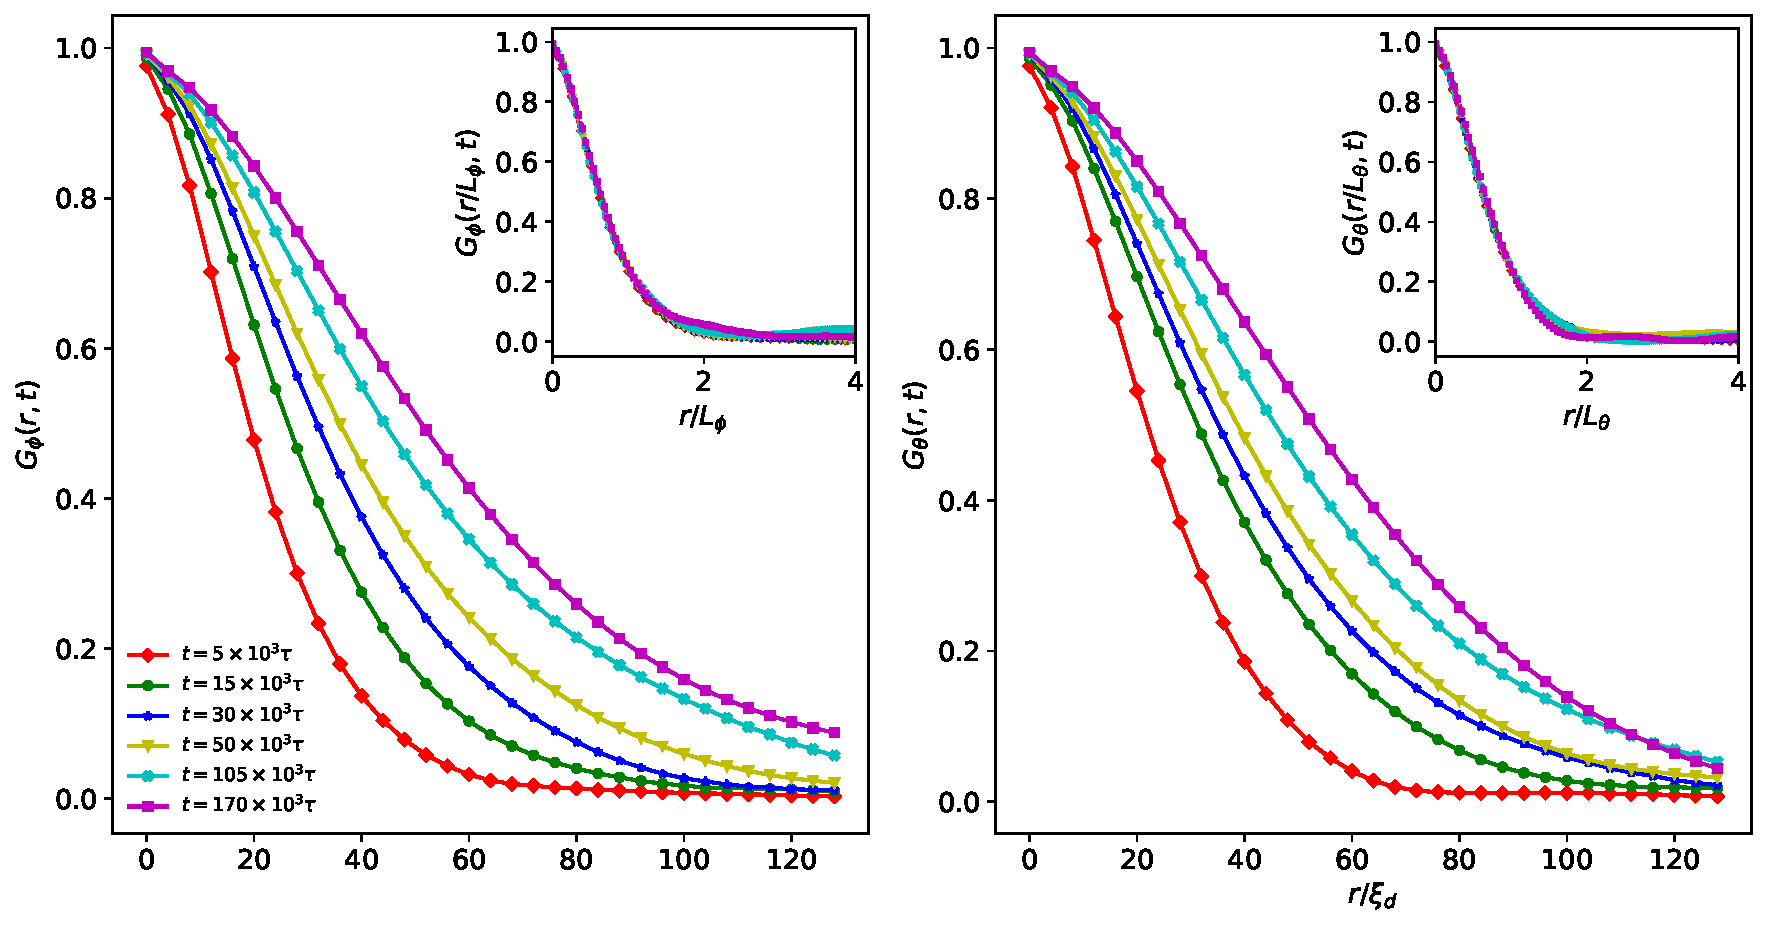
\includegraphics[width=\textwidth]{
            gfx/ch-twoCompDynamics/correlations.pdf}
        \caption{\label{fig:correlation-functions}}
    \end{subfigure}\\
    \begin{subfigure}{0.5\textwidth}
        \centering
        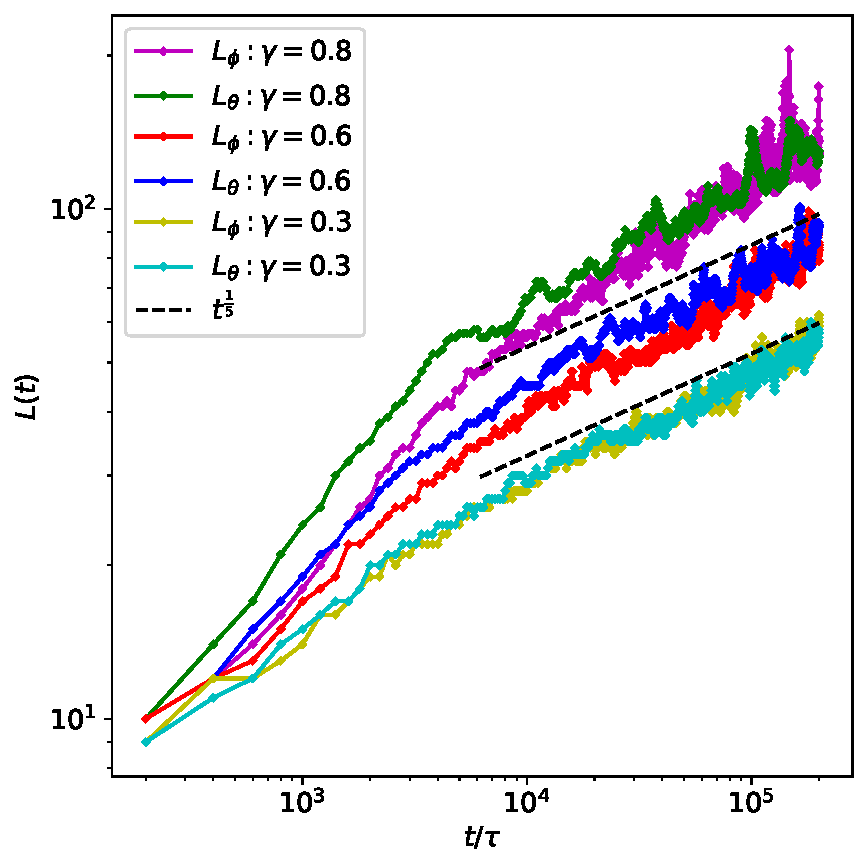
\includegraphics[width=\textwidth]{
            gfx/ch-twoCompDynamics/correlation_lengths.pdf}
        \caption{\label{fig:correlation-lengths}}
    \end{subfigure}
    \begin{subfigure}{0.5\textwidth}
        \centering
        \includegraphics[width=0.8\textwidth]{example-image-a}
        \caption{\label{fig:scalar-vortex-lengths}}
    \end{subfigure}
    \caption{}
\end{figure}
Fig.~\ref{fig:correlation-functions} shows both correlation functions for
\(\gamma=0.6\) for various times through the simulation.
We see that as time increases, the correlation functions extend over larger
distances which indicates that the respective domains are growing over time,
showing long-range order is being established.

From these correlation functions, we may extract a correlation length,
\(L_\delta \) with \(\delta \in \{\Theta, \Phi \} \), that enables us to
determine a length scale over which the correlation function decays.
We take the correlation length to be the value at which the corresponding
correlation function decays to a quarter of its value at
\(r=0\): \(G_\delta(L_\delta, t) = \frac{1}{4}G_\delta(0, t)\).
Using the correlation length, we can determine whether the correlation functions
exhibit dynamical scaling, which implies the form of the functions remains
self-similar at different times throughout the simulation.
This means the function collapses to a universal, time-independent function
when scaled by the correlation length: \(H_\delta(r) = G(r/L_\delta(t), t)\).
The insets of Fig.~\ref{fig:correlation-functions} show the scaling of the
correlation functions when scaled by the respective correlation length.
This confirms that the correlation functions within our system do exhibit
dynamical scaling. \textcolor{red}{Reference to other systems where dynamical
scaling is also seen?} \par
Fig.~\ref{fig:correlation-lengths} shows the correlation lengths for
\(\gamma=0.3\), \(\gamma=0.6\), and \(\gamma=0.8\) as functions of time.
We see that at late times in the evolution, all correlation lengths tend to a
universal \(t^\frac{1}{5}\) scaling.
However, the early-time dynamics are remarkably different for the various
\(\gamma \).
As \(\gamma \) increases, there is a faster growth of the correlation lengths at
early times, which signifies the correlation length being \(\gamma \)-dependent.
\par
We investigate this behaviour by considering the total vortex number of
the system as a function of time.
We can then extract the mean distance between the vortices as
\(\ell_d=1/\sqrt{N_\mathrm{vort}}\), where \(N_\mathrm{vort}\) is the total
number of vortices in the two components.
In a scalar BEC containing an initially large number of vortices, it has been
observed that \(\ell_d \sim t^\beta \)~\cite{Karl2017}, where \(\beta \)
characterizes the annihilation rate of vortices.
In particular, there were two scaling observed: Firstly, a \(\beta=1/5\) scaling
after some short period of evolution.
This scaling is included in Fig.~\ref{fig:correlation-lengths} as a comparison.
Secondly, after a much longer period of evolution, a \(\beta=1/2\) scaling
emerges.
This second scaling can be delayed if the initial vortex distribution is
highly clustered~\cite{Karl2017}.
Fig.~\ref{fig:scalar-vortex-lengths} is a reproduction of both the early- and
late-time scaling of the mean vortex distance, \(\ell_d\), for a scalar system
using the parameters of~\cite{Karl2017}.
We consider three initial conditions: Firstly, we constructed a grid of vortices
analogous to our two-component system (see Sec.~\ref{sec:numerical-setup}).
Secondly, we considered a random distribution of vortices; one with noise
added to the energy spectrum, and one without.
We see that at early and intermediate times, there is a clear \(t^{1/5}\)
scaling in all of the initial states tested.
Furthermore, at late times we recover the \(t^{1/2}\) scaling for all initial
states.
This indicates the scaling is robust and insensitive to the initial conditions.
\par
Motivated by this previous work in scalar BECs, we conduct a similar analysis
on our two-component system containing HQVs, and determine how \(\gamma \)
affects the vortex decay rate.
In particular, we consider the early-time evolution in which
Fig.~\ref{fig:correlation-lengths} suggests interesting dynamics.
\begin{figure}
    \centering
    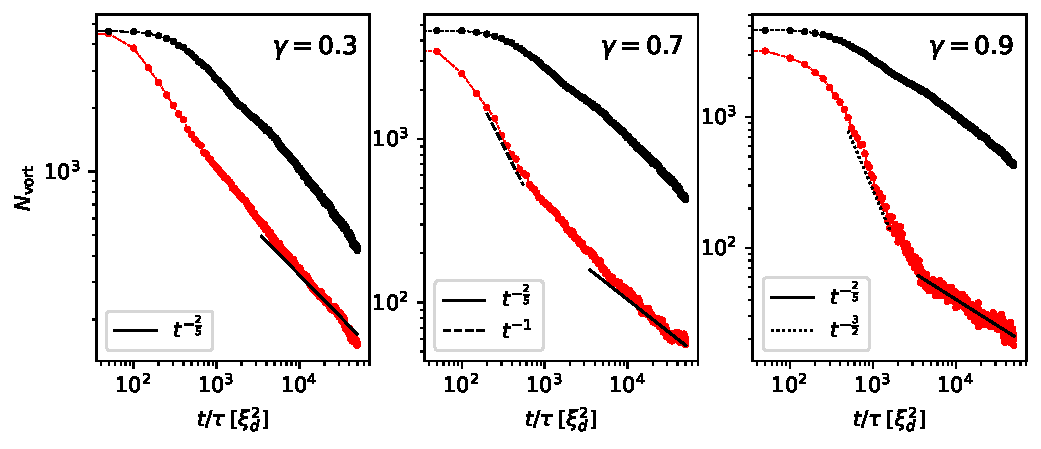
\includegraphics[width=\textwidth]{gfx/ch-twoCompDynamics/vortex_number.pdf}
    \caption{Total vortex number as a function of time for
    \(\gamma=0.3,0.7,0.9\) (red circles).
    Larger \(\gamma \) leads to a faster decay rate of vortices at
    early times due to the rapid annihilation of opposite-signed vortices
    within the same component.\label{fig:vortex-number}}
\end{figure}
The total vortex number is plotted in Fig.~\ref{fig:vortex-number} for
\(\gamma=0.3\), \(\gamma=0.7\), and \(\gamma=0.9\).
We see that for \(\gamma=0.3\), the vortex decay rate is mostly consistent
throughout the evolution, which tends to a \(t^{-2/5}\)
(\(\ell_d \sim t^{1/5}\)) scaling at later times.
More interesting dynamics are revealed for \(\gamma=0.7, 0.9\) where two
different scaling regimes emerge at early times
(\(2.5\times10^2\xi_d^2 \lesssim t/\tau \lesssim 2.5\times10^3\xi_d^2\)) with
\(N_\mathrm{vort} \sim t^{-1}\) for \(\gamma=0.7\) and
\(N_\mathrm{vort} \sim t^{-3/2}\) for \(\gamma=0.9\).
After the initial differing early-time dynamics, the systems then tend to a
universal \(t^{-2/5}\) scaling, which corresponds to \(\ell_d\sim t^{1/5}$
similar to the scalar BEC simulation shown.
These results show a better fit to the theoretical \(t^{1/5}\) scaling than 
indicated by the correlation lengths shown in
Fig.~\ref{fig:correlation-lengths}.
This further suggests that \(L_{\Phi,\Theta}\) differs slightly from \(\ell_d\),
even though the growth of the correlation lengths is driven by vortex
annihilation.
Fig.~\ref{fig:vortex-number} only extends up to \(t/\tau=5\times 10^4\xi_d^2$,
and we expect to see a universal transition to
\(N_\mathrm{vort}\sim t^{-1}\) (\(\ell_d\sim t^{1/2}\)) at much later times for
sufficiently small \(\gamma \).
For large \(\gamma \), due to the rapid annihilation of vortices at early times,
there may not be enough vortices left within the system to facilitate the
transition to the \(N_\mathrm{vort} \sim t^{-1}\) regime.
\par
We wish to investigate further the effect of \(\gamma \) on the initial decay
rate of the vortices.
We can model the vortex decay rate as a simple kinetic-like equation of the form
\begin{equation}
    \pdv{N_\mathrm{vort}}{t} \sim N_\mathrm{vort}^\eta,
\end{equation}
where \(\eta > 1\).
The form of this equation states that the decay rate of the vortices is
dependent on the total number of vortices facilitating the annihilation.
Using this simple model, we can extract a scaling for the total vortex
number as
\begin{equation}
    N_\mathrm{vort} \sim t^{-2/z},
    \label{eq:vortex-number-scaling}
\end{equation}
where \(z=-2(1-\eta)\).
An exponent of \(z=2\) corresponds to a two-body collision process, in which
only two vortices are required to annihilate.
On the contrary, an exponent of \(z=5\) corresponds to a three-body collision
process, where three vortices are necessary to facilitate annihilation.
\begin{figure}[t!]
    \centering
    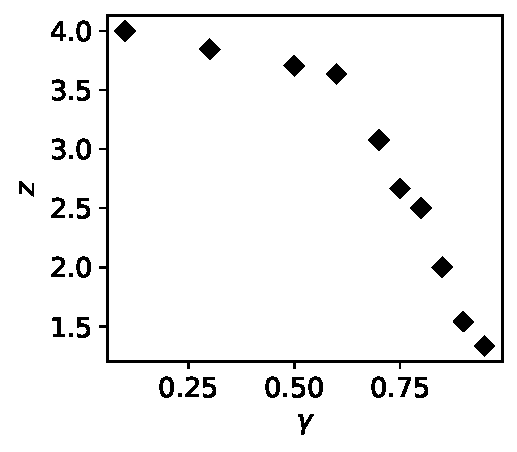
\includegraphics{gfx/ch-twoCompDynamics/gamma_vs_expo.pdf}
    \caption{The exponent \( z \) in Eq.~\eqref{eq:vortex-number-scaling} as a
    function of \(\gamma \).
    We see that after \(\gamma \gtrsim 0.6\) a rapid decrease of the exponent
    occurs, signalling a rapid change in vortex
    dynamics.\label{fig:exponent-vs-gamma}}
\end{figure}
Fig.~\ref{fig:exponent-vs-gamma} shows the exponent, \( z \), as a function of
\(\gamma \) where \( z \) is extracted within the time interval
\(2.5 \times 10^2\xi_d^2 < t/\tau < 2.5\times10^3\xi_d^2\).
We see a rapid decrease of the exponent after \(\gamma \gtrsim 0.6\), in which
Fig.~\ref{fig:vortex-number} shows the rapid annihilation of vortices is
prevalent.
The decrease of the exponent in our simulations signals an additional vortex
interaction mechanism not present in scalar BEC systems.

\subsection{HQV dipole dynamics}
Numerous studies have been conducted to try and understand the inter-vortex
forces between HQVs in two-component systems~\cite{Eto2011, Kasamatsu2016}.
In particular, Kasamatsu \textit{et.\ al.}~\cite{Kasamatsu2016} tried to derive a
point vortex model to explain the dynamics shown in
Fig.~\ref{fig:exponent-vs-gamma} but found that the model failed to accurately
predict in vortex dynamics.
We can discern more about the dynamics of these HQVs by considering dipole
motion.


As a simple test case, I consider two HQVs of opposite winding within the same
component.
The vortices are placed in a uniform system

\chapter{\label{chap: spin-1}Generalised Kibble-Zurek scaling in a spin-1
Bose-Einstein condensate}

Nonequilibrium phase transitions are ubiquitous, arising in many areas of
physics, including cosmology~\cite{Kibble1980,Mazumdar2019}, condensed
matter~\cite{Chuang1991,Hendry1994,Bauerle1996,Ruutu1996,Sondhi1997,
Polkovnikov2011}, and ultracold atomic gases~\cite{Hadzibabic2006,Langen2015,
Fletcher2015,Liu2018}.
A quantum phase transition (QPT), in contrast to its classical counterpart, is a
zero-temperature transition driven by quantum fluctuations~\cite{Sachdev2011}.
In such a transition, a fundamental change of ground state occurs as an external
parameter is varied across the quantum critical point.
For a continuous phase transition, as this critical point is passed, the
timescale governing the dynamics diverges, resulting in the system no longer
adiabatically following the ground state.
This non-adiabatic evolution implies that the symmetry of the system is broken
independently in causally disconnected regions, which typically results in the
formation of topological defects.
The Kibble-Zurek mechanism (KZM) is a theory that describes the resulting
dynamics and predicts the scaling properties of the excitations from the details
of the universality class of the transition.
It was first introduced by Kibble in the context of cosmological phase
transitions in the early universe~\cite{Kibble1976, Kibble1980}, before being
extended by Zurek to condensed matter systems~\cite{Zurek1985, Zurek1993,
    Zurek1996}.

Any continuous phase transition can be modelled using the KZ theory, and due to
this robustness, it has been successfully applied to both
classical~\cite{Donadello2016,Beugnon2017} and
quantum~\cite{Dziarmaga2005, Damski2005, Lamacraft2007} phase transitions.
Whilst the theory has had great success in applications to continuous,
second-order transitions, direct application to discontinuous phase transitions
does not typically give an accurate description of observed scaling laws.
This is due to the fact that at the critical point of a continuous phase
transition the energy spectrum is gapped, in which well-defined correlation
lengths and time scales can be derived.
In a first-order, discontinuous phase transition, the energy spectrum at the
critical point is gapless, and hence the traditional KZ theory breaks down.
Recently, there has been the first experimental evidence of the existence of
scaling laws for a first-order QPT~\cite{Qiu2020}, where standard KZ theory
failed to predict the observed scaling.
However, the KZM was generalised by considering the energy gap between the
metastable state and its first corresponding excited state, which then gave an
accurate prediction of the observed scaling laws.
There is current interest in trying to generalise the KZM and applying it to
discontinuous transitions and deriving appropriate scaling
laws~\cite{Divakaran2008, Suzuki2015}.

The seminal work of Fisher and Berker~\cite{Fisher1982}, in the classical case,
first discussed a particular type of discontinuous, first-order transition and
introduced the notion of a discontinuous critical point (DCP).
Such a DCP separates two distinct phases, characterized by a discontinuous jump
in the order parameter.
Despite the discontinuity, the transition can still be characterized by a
diverging length scale and hence critical exponents can be derived.
This framework was then extended to the quantum case, specifying the conditions
for a discontinuous quantum critical point (DQCP)~\cite{Suzuki2015}.
The DQCP leads to a prediction of the scaling of the defect density that is
modified from the typical KZ scenario.

Spinor BECs offer a highly controllable platform for studying non-equilibrium
physics, ranging from topological defects~\cite{Lovegrove2014, Borgh2016} to
quantum quenches~\cite{Symes2017, Prufer2018, Schmied2019}.
In addition, their rich phase diagram has seen the KZM applied both numerically
and experimentally in various continuous phase transitions~\cite{Damski2007,
    Saito2007, Saito2007a, Swislocki2013, Witkowska2013, Anquez2016}.
For a ferromagnetic spin-1 BEC, there exists a first-order QPT between a
three-component broken-axisymmetry (BA) phase and a ferromagnetic (FM) phase,
making this system an ideal platform for investigating the KZM across
discontinuous transitions.

In this Chapter we analytically and numerically investigate the KZM in a 1D FM
spin-1 BEC\@.
By quenching the quadratic Zeeman shift, we are able to quench the system
through both continuous and discontinuous phase transitions.
In particular, we first examine the resulting scaling laws associated with
quenching through the continuous phase transition from the polar phase to the
BA phase, and confirm that these are in excellent agreement with the KZ theory.
Then, we extend the KZM to predict the scaling laws of the discontinuous,
first-order phase transition between the BA and FM phases.
Quenching the quadratic Zeeman shift allows the system to change from the
BA phase into a phase-separated FM phase, where domains with opposing
condensate-spin projection develop~\cite{Kawaguchi2012}.
We show that, despite this particular transition having a gapless spectrum, the
standard KZ theory can be generalised and extended to cover discontinuous,
first-order transitions.
In addition, scaling behaviour near the critical point is derived by means of
linearising the mean-field equations for the spin-1
condensate~\cite{Damski2007, Uchino2010}.
Predicted scaling laws are then confirmed by direct numerical simulations.

\section{The Kibble-Zurek mechanism}\label{sec: the-KZM}
Consider a system that undergoes a spontaneous breaking of symmetry when a
control parameter, \( \lambda \), is ramped across a phase transition that
occurs at the critical point, \( \lambda_c \).
A continuous, second-order phase transition can be characterized by a divergence
of the equilibrium correlation length~\cite{DelCampo2014}
\begin{equation}
    \xi(\epsilon) \sim |\epsilon|^{-\nu},
\end{equation}
and an equilibrium relaxation time
\begin{equation}
    \tau(\epsilon) \sim \xi^z \sim |\epsilon|^{-\nu z},
    \label{eq: equil-relax-time}
\end{equation}
where
\begin{equation}
    \epsilon = \frac{\lambda - \lambda_c}{\lambda_c}
\end{equation}
is the dimensionless distance from the critical point.
The equilibrium relaxation time \( \tau \) describes the time it takes for the
system to react to an external change of a parameter.
In a quantum phase transition, the relaxation time is set by the inverse of an
energy gap \( \Delta \) between the ground state and the first excited
state~\cite{Zurek2005, Damski2006}
\begin{equation}
    \tau \simeq \Delta^{-1}.
\end{equation}
As we approach the critical point, the energy gap vanishes as
\begin{equation}\label{eq: delta-epsilon-relation}
    \Delta \sim |\epsilon|^{\nu z}.
\end{equation}
The system is initially prepared in a high-symmetry phase (\(  \epsilon > 0 \)),
but breaks that symmetry as the critical point is crossed (\(  \epsilon < 0 \)).
In the above equations, the exponents \(  z \) and \( \nu \) are the dynamical
and correlation length critical exponents, respectively.
Different systems which have the same critical exponents are said to belong
to the same universality class~\cite{Sachdev2011,DelCampo2014}.

The KZM describes the dynamics of crossing the critical point when \( \lambda \)
is continually varied.
We assume the form of a linear quench (cases concerning non-linear quenches are
discussed in Refs.~\cite{Barankov2008,Mondal2009}), such that the control
parameter can be written as
\begin{equation}
    \lambda(t) = \lambda_c\left[1 - \epsilon(t)\right],
\end{equation}
where the distance to the critical point is
\begin{equation}
    \epsilon(t) = \frac{t}{\tau_Q},
    \label{eq: time-dependent-epsilon}
\end{equation}
for a quench time \( \tau_Q \).
This form gives a transition rate \( |\dot{\epsilon}/{\epsilon}|=t^{-1} \) which
diverges as we approach the critical point.
Here, \( t \in [-\tau_Q, \tau_Q] \), where the critical point is reached at
\( t=0 \).
The dynamics of the system can be broken into three stages as \( \epsilon \) is
ramped from \( \epsilon > 0 \) to \( \epsilon < 0 \): adiabatic, frozen, and
adiabatic again (see Fig.~\ref{fig: adiabatic-impulse} for a schematic
representation).
\begin{figure}
    \centering
    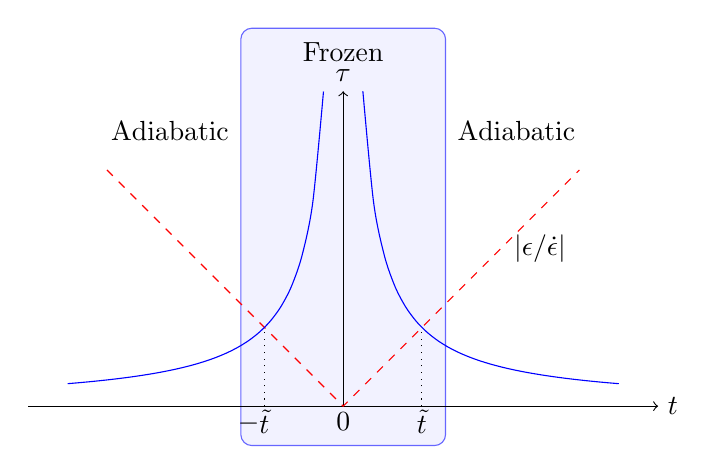
\begin{tikzpicture}
        \filldraw[color=blue!60, fill=blue!5, rounded corners] (-1.3, -0.5)
        rectangle (1.3, 4.8);
        \draw[->] (-4, 0) -- (4, 0) node[right] {\( t \)};
        \draw[->] (0, 0) -- (0, 4) node[above] {$\tau$};
        \draw[scale=1, domain=-3:3, dashed, variable=\x, red] plot
        ({\x}, {abs(\x)});
        \draw[scale=1, domain=0.25:3.5, smooth, variable=\x, blue] plot
        ({\x}, {\x^(-1)});
        \draw[scale=1, domain=-3.5:-0.25, smooth, variable=\x, blue] plot
        ({\x}, {abs(\x^(-1))});
        \node at (1, -0.2) {\( \tilde{t} \)};
        \node at (-1, -0.2) {\( \tilde{t} \)};
        \node at (-1.2, -0.22) {$-$};
        \draw[dotted] (1, 0) -- (1, 1);
        \draw[dotted] (-1, 0) -- (-1, 1);
        \node at (0, 4.5) {Frozen};
        \node at (2.5, 2) {$|\epsilon/\dot{\epsilon}|$};
        \node at (2.2, 3.5) {Adiabatic};
        \node at (-2.2, 3.5) {Adiabatic};
        \node at (0, -0.2) {$0$};
    \end{tikzpicture}
    \caption[Schematic representation of the dynamics of a system during a
        linear quench]
    {A schematic representation of the dynamics of a system during a
    linear quench. The system starts in a high-symmetry phase (\( t > 0 \)) and
    is quenched across a critical point to a low symmetry phase (\( t < 0 \)) by
    the reduced control parameter (red dashed line) \( \epsilon(t) = t/\tau_Q\).
    As the critical point is approached, the equilibrium relaxation time
    (blue line) diverges, and the order parameter can no longer follow the
    ground state, leading to frozen dynamics in the interval
    \( t \in [-\tilde{t}, \tilde{t}] \)}.\label{fig: adiabatic-impulse}
\end{figure}

Far from the critical point, the equilibrium relaxation time is small compared
to the inverse transition rate \( |\epsilon/\dot{\epsilon}| \), meaning the
system adiabatically follows the instantaneous ground state for \(\epsilon(t)\).
This stage of adiabaticity lasts until the relaxation time becomes comparable
to \(|\epsilon / \dot{\epsilon}|\):
\begin{equation}
    \tau \approx |\epsilon/\dot{\epsilon}|=\tilde{t}.
    \label{eq: freeze-out-equal}
\end{equation}
Using Eqs.~\eqref{eq: delta-epsilon-relation}
and~\eqref{eq: time-dependent-epsilon}, the above equation can be solved to
yield the freeze-out time, \( \tilde{t} \):
\begin{equation}
    \tilde{t} \sim \tau_Q^\frac{z\nu}{1 + z\nu}.
    \label{eq: freeze-out-scaling}
\end{equation}
After the freeze-out time is passed, however, the relaxation time diverges and
the system can no longer keep up with the externally imposed changes.
The system then enters the so-called impulse regime, where the dynamics are
frozen and remains in this regime until \( -\tilde{t} \), when the relaxation
time becomes faster than the transition rate once again.
The consequence of the impulse region, however, is that the system arrives at
\( -\tilde{t} \), in which the true ground state is in a broken-symmetry phase,
whilst remaining in the state set at \( \tilde{t} \), which corresponds to a
symmetric phase.
This state at \( \tilde{t} \) then becomes the initial state for the last
adiabatic stage of evolution beginning at \( -\tilde{t} \).
At this point, the system is no longer in its current ground state and rectifies
this by breaking the symmetry of the initial state.
This results in the formation of distinct domains in the system whose size is
set by the value of the equilibrium correlation length at the freeze-out time
\begin{equation}
    \hat{\xi}=\xi(\tilde{t}) \sim \tau_Q^{\frac{\nu}{1 + z\nu}}.
    \label{eq: KZM-domain-size}
\end{equation}
If the system supports topological defects such as vortices, then the defect
density is given by
\begin{equation}\label{eq: KZM-defects-scaling}
    N_d \simeq \hat{\xi}^{-d} \sim \tau_Q^{\frac{-d\nu}{1+z\nu}},
\end{equation}
where \( d \) is the number of spatial dimensions.
This key provides a foundation in testing the KZM in subsequent sections, and
has already been successfully applied to numerous spinor BEC
systems~\cite{Damski2007, Swislocki2013, Anquez2016, Saito2007, Saito2007a} to
determine the validity of the KZM\@.

\section{Numerical studies of the Kibble-Zurek mechanism across a second-order
quantum phase transition}
To verify the key results of the KZ theory presented in the previous section,
we perform numerical simulations using a spin-1 BEC\@.
As shown in Sec.~\ref{sec: ground-states-spin-1}, there are four ground state
phases of spin-1 BECs; namely, the ferromagnetic, partially-magnetised polar,
polar, and broken-axisymmetry phases, where each ground state phase has an
associated symmetry.
The Kibble-Zurek mechanism can be studied in spin-1 BECs by considering how
the change of a control parameter causes the order parameter to change from
one ground state to another.
As it does this, the symmetry of the system is spontaneously broken, and hence
the Kibble-Zurek theory can be applied.

Spin-1 BECs support numerous first- and second-order quantum phase transitions
when the linear, \( p \), or quadratic, \( q \), Zeeman shifts are
ramped across a critical point~\cite{Kawaguchi2012}.
A second-order quantum phase transition is characterised by the continuous first
derivatives of the internal energy with respect to variations in \( p \) and
\( q \) at the critical point.
In this section, we aim to test the predictions of the Kibble-Zurek mechanism
for a second-order quantum phase transition in a spin-1 BEC\@.

\subsection{\label{sec: KZM-second-order-numerics}Polar to broken-axisymmetry
quench}
Motivated by previous work~\cite{Damski2007}, we will investigate the
Kibble-Zurek mechanism across the second-order phase transition occurring
between the polar and broken-axisymmetry phases in a ferromagnetic spin-1 BEC\@.
The polar phase is the energetic ground state when \( Q=q/|c_1|n > 2 \).
The critical point \( Q = 2 \) (for \(p=0\)) represents the second-order phase
transition to the BA phase.
The BA phase contains three Bogoliubov modes~\cite{Uchino2010}, but only one
is non-zero in the long wavelength limit (see
Sec.~\ref{subsec: bogoliubov-modes} for further details on Bogoliubov modes in
a spin-1 BEC).
This mode is gapped, and has the scaling form
\begin{equation}
    \Delta \sim \sqrt{4 - Q^2}.
\end{equation}
We temporally vary \(Q\) according to
\begin{equation}
    Q(t) = 2 - \frac{t}{\tau_Q},
    \label{eq: time-dep-Q-damski}
\end{equation}
where \( \tau_Q^{-1} \) is the quench rate.
To investigate Kibble-Zurek scaling, we consider the freeze-out time,
\( \tilde{t} \), which occurs when the equilibrium relaxation time is equal to
the rate of change of the control parameter [see
Eq.~\eqref{eq: freeze-out-equal}].
Using the above form of the linear quench, the freeze-out time is calculated
as~\cite{Damski2007}
\begin{equation}
    \tilde{t} \sim \tau_Q^{1/3}.
\end{equation}

We now analyse the resulting dynamics when linearly decreasing \( Q \) according
to Eq.~\eqref{eq: time-dep-Q-damski}, starting from the polar phase (\(t < 0\))
and end the simulation precisely at \( Q = 0 \) (\( t=2\tau_Q \)) in the BA
phase.
The initial state is a polar wave function that is slightly perturbed:
\begin{equation}
    \psi = \left(\delta\psi_1, \frac{1}{\sqrt{L}} + \delta\psi_0,
    \delta\psi_{-1}\right),
    \label{eq: peturbed-polar-initi-state}
\end{equation}
where \( |\delta\psi_m| \ll 1 / \sqrt{L} \) are small noise terms and \( L \) is
the length of the computational domain.
The real and imaginary parts of these terms at individual grid points are drawn
from the probability distribution
\( p(x) = \exp(-x^2/2\sigma^2)/\sqrt{2\pi}\sigma \).
To ensure we remain close to the polar ground state, we take
\( \sigma=10^{-4} \).
We consider a 1D system with \(N_x = 2048\) grid points with \(L=78\) and
choose dimensionless spin-independent interaction \(c_0=1.4\times10^5\) and
\(c_0/c_1 = -222\).
Note that these choice of parameters give a condensate close to that of
\(^{87}\)Rb, in which \(c_0/c_1 \approx -111\) (see
Sec.~\ref{subsec: experimental-params}).
We start with the initial state in Eq.~\eqref{eq: peturbed-polar-initi-state}
and integrate the spin-1 Gross-Pitaevskii equations~\cite{Symes2016}.

\subsection{Evolution of the transverse magnetisation}
To determine the freeze-out time within our system, we need to find a quantity
that grows as the transition point is crossed.
This freeze-out time is then measured by the time it takes for the onset of
that growth to occur.
The quantity that satisfies this condition in the polar to BA transition is the
transverse magnetisation
\begin{equation}
    M_\perp = \int \langle F_x^2\rangle + \langle F_y^2\rangle \, \dd z,
\end{equation}
where \(F_x\) and \(F_y \) are the \(x, y\) components of the condensate spin
vector, respectively.
In the polar phase this quantity is zero, but becomes non-zero in the BA limit
where it is \(M_\perp = (1 - Q^2/4)/L\).
\begin{figure}
    \centering
    \begin{subfigure}{0.49\textwidth}
        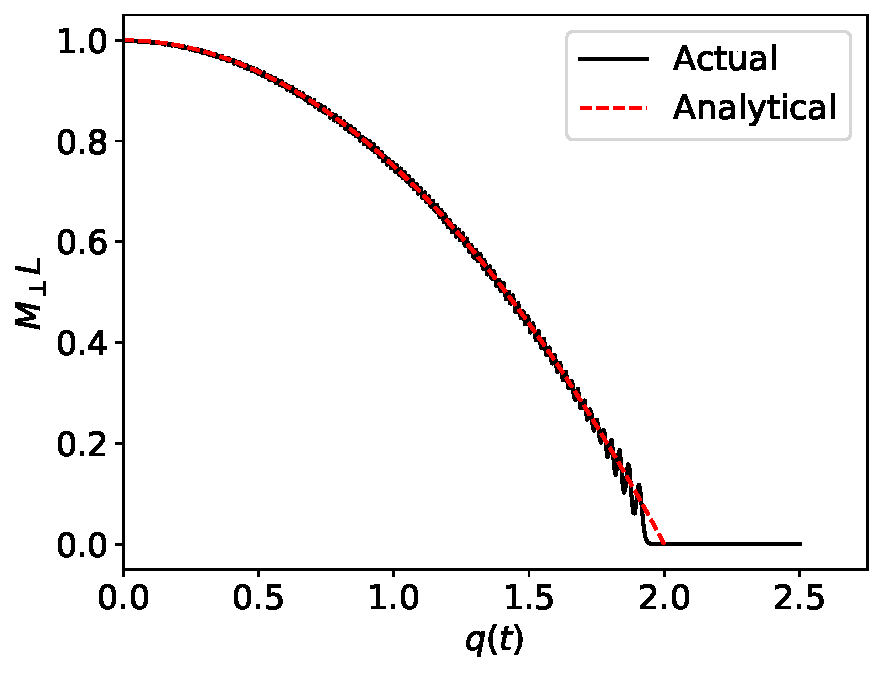
\includegraphics[width=\textwidth]{gfx/ch-spin1/magnetisation_vs_Q.pdf}
        \caption{\label{subfig: magnetisation-vs-Q}}
    \end{subfigure}
    \begin{subfigure}{0.49\textwidth}
        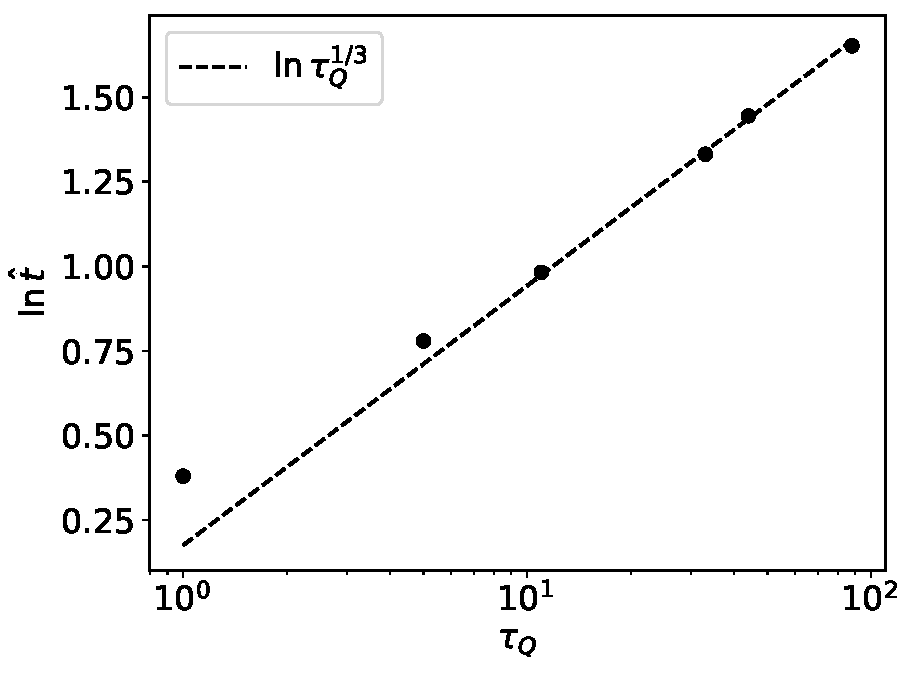
\includegraphics[width=\textwidth]{gfx/ch-spin1/t-hat_vs_tau_q.pdf}
        \caption{\label{subfig: t-hat-vs-tau-q}}
    \end{subfigure}
    \caption[Transverse magnetisation for as a function of quench parameter,
        \(Q\)]
    {(a) The transverse magnetisation as a function of \( Q(t) \) for
        \(\tau_Q=11\).
        Plotted are the numerical values (black line) and the
        analytical prediction (red line).
        (b) The extracted value of \( \tilde{t} \) versus the quench time.
        Overlaid is the power-law scaling \(\tau_Q^{1/3}\).}
\end{figure}
Fig.~\ref{subfig: magnetisation-vs-Q} shows a typical evolution of the
transverse magnetisation for \(\tau_Q = 11\).
One sees that after the critical point is crossed at \( Q = 2 \), the transverse
magnetisation grows in a non-trivial fashion.
This growth starts precisely after the system exits the freeze-out stage, which
occurs at \(t=\tilde{t}\).
The magnetisation then grows rapidly, exceeding the analytical prediction at
certain time intervals, and begins to oscillate with the amplitude of the
oscillation decaying over time.
Using this quantity, we can test the Kibble-Zurek prediction in
Eq.~\eqref{eq: freeze-out-scaling}.

We define \( \tilde{t} \) as the instant when \(M_\perp L\) intersects 1\% of
the maximum value given by \(M_\perp L = 1\).
Fig~\ref{subfig: t-hat-vs-tau-q} shows the extracted value of \( \tilde{t} \)
for a range of \( \tau_Q \).
We see an unambiguous power-law scaling of \(\tau_Q^{1/3}\) for
\(\tau_Q \geq 10\).
The gradual departure from the \(\tilde{t} \sim \tau_Q^{1/3}\) scaling indicates
that the quench has to be sufficiently slow to capture the Kibble-Zurek scaling.
We note that the choice of the 1\% threshold used here is arbitrary.
We have tested a range of values up to a maximum of 10\%, and obtain
quantitatively similar behaviour for all values tested.

\section{Extending the Kibble-Zurek theory to first-order quantum phase
transitions}
The preceding sections were concerned with the KZM across second-order phase
transitions.
Describing the KZM across discontinuous, first-order transitions, however, has
been difficult due to lack of
universality~\cite{Turban2002,Continentino2004,Nauenberg1975}.
More recent work has aimed to bridge the gap between the KZM and first-order
transitions~\cite{Suzuki2015}, and here we present an overview of how the KZM
can be adapted to describe a discontinuous phase transition that will form the
focus in the remainder of this chapter.

Fisher and Berker~\cite{Fisher1982} demonstrated that first-order phase
transitions occurring at a DCP can also give rise to scaling behaviour.
Such a DCP results in a discontinuity in the order parameter as the critical
point is passed.
Despite this, the transition can still be characterised by a divergent length
scale, and hence, critical exponents can be derived.
Suzuki \textit{et al.}~\cite{Suzuki2015} aimed to extend the notion of a DCP to
a DQCP\@.

Let us consider a system that contains a critical point at
\( q = q_c \), where \( q \) is a tunable parameter and contains
the presence of a symmetry-breaking field, \( p \).
For one to have a DQCP five conditions need to be satisfied~\cite{Suzuki2015}.
Firstly, the energy density \( \epsilon(q, p) \) must be a continuous
function of \( q \) and \( p \) across the critical point
\begin{equation}
    \epsilon(q_c + 0, 0) = \epsilon(q_c - 0, 0).
    \label{eq: continuous-energy-cond}
\end{equation}
The derivative of this energy density, however, is discontinuous
\begin{equation}
    \pdv{\epsilon(q_c + 0, 0)}{q} \neq \pdv{\epsilon(q_c - 0, 0)}{q}.
\end{equation}
The order parameter \( m(q, p) \), where \( m=-\pdv{\epsilon(q, p)}{p} \)
has a discontinuous jump as a function of \( q \) as the critical point is
passed
\begin{equation}
    |m(q_c - 0, 0)| > m(q_c + 0, 0)| = 0,
\end{equation}
whilst also having a discontinuous jump as a function of \( p \)
\begin{equation}
    |m(q_c, \pm 0)| > 0.
\end{equation}
Finally, we require that the derivative of the energy density be bounded as
\( q \rightarrow q_c \pm 0 \)
\begin{equation}
    \left|\pdv{\epsilon(q_c \pm 0, 0)}{q}\right| < \infty.
    \label{eq: bounded-energy-derivative-cond}
\end{equation}
These five conditions encapsulate a DQCP\@.

\subsection{BA to FM transition as a DQCP}
Let us now consider a specific example.
We are interested in the phase transition that occurs between the
broken-axisymmetry (BA) and ferromagnetic (FM) phases.
The energy densities for the two states are given by~\cite{Kawaguchi2012}
\begin{equation}
    \epsilon_\mathrm{BA} = \frac{{(-p^2 + q^2 +2qc_1n)}^2}{8c_1nq^2}
    + \frac{1}{2}c_0n, \qquad
    \epsilon_\mathrm{FM_{\pm}} = \mp p + q + \frac{1}{2}n(c_0 + c_1),
\end{equation}
where \( \epsilon_\mathrm{FM_{\pm}} \) corresponds to the energy density in the
FM phase for the spinor \( \zeta = {(1, 0, 0)}^T \) (+) and
\( \zeta = {(0, 0, 1)}^T \) (-).
One sees that at the critical point \( q=q_c=0 \) and \( p=0 \) the energy is
continuous.
On the other hand, the derivative of the above energies with respect to \( q \)
yields
\begin{equation}
    \pdv{\epsilon_\mathrm{BA}}{q} =
    \frac{1}{4c_1n}\left(q - \frac{p^4}{q^3}\right) - \frac{p^2}{q^2}
    + \frac{1}{2},
    \qquad
    \pdv{\epsilon_\mathrm{FM_{\pm}}}{q} = 1.
\end{equation}
Indeed, there is a discontinuity in these derivatives at \( q=p=0 \), although
they still remain bounded.
The relevant order parameters for this transition are given by
\begin{equation}
    m_\mathrm{BA} = \frac{p(p^2 - q^2 - 2qc_1n)}{8c_1nq},
    \qquad
    m_{\mathrm{FM}_{\pm}} = \pm 1,
\end{equation}
which is precisely the local magnetisation, \(F_z = |\psi_1|^2
- |\psi_{-1}|^2\), in both phases (see Sec.~\ref{sec: ground-states-spin-1}).
Again, one sees that at the critical point and for \( p=0 \) the order parameter
becomes zero in the BA phase whilst becoming non-zero in the FM phase.
In addition, as the linear Zeeman shift \( p \) is varied both above and below
zero, the order parameter becomes non-zero.
We have shown that the BA to FM phase transition satisfies all conditions
specified in Eqs.~\eqref{eq: continuous-energy-cond}
-\eqref{eq: bounded-energy-derivative-cond}
and therefore is a DQCP\@.

\subsection{Determining the relevant Bogoliubov mode}\label{subsec: bogoliubov-modes}
In order to determine the relevant energy spectrum for our system, we consider
the Bogoliubov modes of the BA phase of a spin-1 BEC, which we derive explicitly
from the relevant Bogoliubov transformations.
The broken-axisymmetry phase can be parameterised as~\cite{Uchino2010}
\begin{align}
    \zeta^\text{BA} = \left(\frac{\sin\theta}{\sqrt{2}}, \cos\theta,
    \frac{\sin\theta}{\sqrt{2}}\right),
\end{align}
where \(\sin\theta = \sqrt{1/2+q/(4nc_1)}\).
The fluctuation operators for this state are then defined as~\cite{Uchino2010}:
\begin{align}
    \hat{a}_{\vb{k}, d} &= \frac{\sin\theta}{\sqrt{2}}(\hat{a}_{\vb{k}, 1}
    + \hat{a}_{\vb{k}, -1}) + \cos\theta \hat{a}_{\vb{k}, 0}, \\
    \hat{a}_{\vb{k}, f_z} &= \frac{1}{\sqrt{2}}(\hat{a}_{\vb{k}, 1}
    - \hat{a}_{\vb{k}, -1}), \label{eq: a_k-fz}\\
    \hat{a}_{\vb{k}, \theta} &= \frac{\cos\theta}{\sqrt{2}}(\hat{a}_{\vb{k}, 1}
    + \hat{a}_{\vb{k}, -1}) - \sin\theta \hat{a}_{\vb{k}, 0},
\end{align}
where on the right-hand side \(\hat{a}_{\vb{k}, m}\) is the annihilation
operator for a spin-\(1\) boson in magnetic level \(m\) (for \(m=-1,0,+1\)),
determined by expanding the wave function field operator as
\begin{align}
    \hat{\psi}_m(\vb{x}) = \frac{1}{\sqrt{V}}\sum_{\vb{k}}
    \hat{a}_{\vb{k}, m}e^{i\vb{k}\cdot \vb{x}},
\end{align}
where \(V\) is the volume of the system.

The sub-Hamiltonian for the spin fluctuation mode \(\hat{a}_{\vb{k}, f_z}\) can
be diagonalised using the transformation
\begin{align}
    \hat{b}_{\vb{k}, f_z} = \sqrt{\frac{\epsilon_{\vb{k}} + q/2
    + E_{\vb{k}, f_z}}{2E_{\vb{k}, f_z}}}\hat{a}_{\vb{k}, f_z}
    + \sqrt{\frac{\epsilon_{\vb{k}} + q/2 - E_{\vb{k}, f_z}}{2E_{\vb{k}, f_z}}}
    \hat{a}_{-\vb{k}, f_z}^\dagger,
\end{align}
where \(\epsilon_{\vb{k}} = \hbar^2|\vb{k}|^2/2M\) is the kinetic energy.
The Bogoliubov spectrum is then given by
\begin{align}\label{eq: e_k-fz}
    E_{\vb{k}, {f_z}} = \sqrt{\epsilon_{\vb{k}}(\epsilon_{\vb{k}} + q)}.
\end{align}
The sub-Hamiltonians for the density fluctuation mode \(\hat{a}_{\vb{k}, d}\)
and the \(\theta \) mode
\(\hat{a}_{\vb{k}, \theta}\) can be similarly diagonalised using operators
\(\hat{b}_{\vb{k}, +}\) and \(\hat{b}_{\vb{k}, -}\), which yields the remaining
two Bogoliubov modes~\cite{Uchino2010}:
\begin{align}\label{eq: e_k-pm}
    E_{\vb{k}, \pm}= \sqrt{\epsilon_{\vb{k}}^2 + n(c_0-c_1)\epsilon_{\vb{k}}
        + 2{(nc_1)}^2(1 - \tilde{q}^2) \pm E_1(\vb{k})},
\end{align}
where \(\tilde{q} = -q/2c_1n\) and
\begin{align}
    E_1(\vb{k}) = \sqrt{{\left[n{(c_0 + 3c_1)}\epsilon_{\vb{k}}
                    + 2{(c_1n)}^2(1-\tilde{q}^2)\right]}^2
        - 4c_1(c_0+2c_1){(n\tilde{q}\epsilon_{\vb{k}})}^2}.
\end{align}
The final, diagonalised Hamiltonian then reads
\begin{align}
    \hat{H}^\text{BA} =\, E_0^\text{BA}
    + \sum_{\vb{k} \neq 0}\left[E_{\vb{k}, f_z}\hat{b}^\dagger_{\vb{k}, f_z}
    \hat{b}_{\vb{k}, f_z}
    + E_{\vb{k}, -}\hat{b}^\dagger_{\vb{k}, -}\hat{b}_{\vb{k}, -}
    + E_{\vb{k}, +}\hat{b}^\dagger_{\vb{k}, +}\hat{b}_{\vb{k}, +}\right],
\end{align}
where \(E_0^\text{BA}\) is the ground state energy for the
BA phase~\cite{Uchino2010}.

For simplicity, we now consider a 1D system.
In the long-wavelength limit (\(k \rightarrow 0\)), the only non-zero (gapped)
mode is given by \(E_{k, +}= \sqrt{4{(c_1n)}^2(1-\tilde{q})}\), which has the
form \(E_{k, +} \sim \sqrt{{q_c^\prime}^2 - q^2}\), where
\(q_c^\prime = 2c_1n\).
The relevant mode for the BA to FM transition can be found by considering the
imaginary parts of the derived Bogoliubov energies (see
Fig.~\ref{fig: dens-spin-energies}).
\begin{figure}[tb]
    \centering
    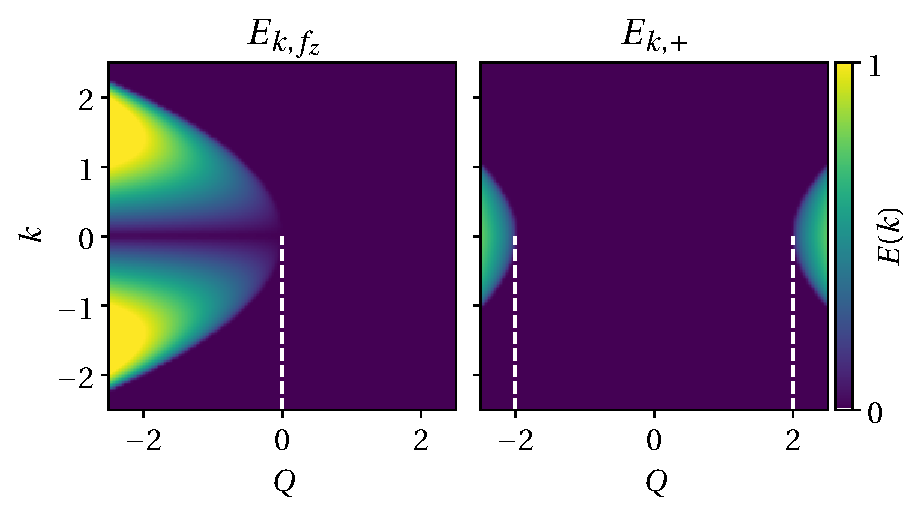
\includegraphics[width=0.75\textwidth]{gfx/ch-spin1/bogoliubov_energies.pdf}
    \caption[Real and imaginary parts of the Bogoliubov energies for the
        broken-axisymmetry phase of a spin-1 BEC]
    {\label{fig: dens-spin-energies}Imaginary parts of the energies defined in
    Eq.~\eqref{eq: e_k-fz} and Eq.~\eqref{eq: e_k-pm} in a parameter space of
    mode \(k\) and \( Q=q/|c_1|n \).
    Note that \(E_{k, -} = 0\) for our range of \(k\) and hence is not shown.}
\end{figure}
For \(|Q|>2\), \(\text{Im}(E_{k, +})\) becomes non-zero, indicating an
instability.
The critical point \(Q = 2\) corresponds to the second-order phase transition
from the polar to the BA phase, indicating that \(E_{k, +}\) is the desired
Bogoliubov energy for that particular transition.
However, we see that for \(Q<0\) the imaginary part of \(E_{k, f_z}\) becomes
non-zero, and hence unstable.
This critical point corresponds to the transition between the BA and FM phases,
which precisely describes our transition of interest.
Therefore, \(E_{k, f_z}\) is the correct Bogoliubov mode for our transition.
Note that for \(k=0\) an instability does not occur in the \(E_{k, f_z}\) mode,
and so studies focussing on this mode in particular (the so-called uniform mode
approximation) will not capture the phase transition that occurs at
\(Q=0\)~\cite{Matuszewski2009, Qiu2020, Mirkhalaf2021}.
In contrast, choosing the \(k=0\) mode is sufficient to capture the phase
transition at \(Q=2\) since it is the most unstable mode indicated in
\(E_{k, +}\).
In practice, the \(Q=-2\) transition is not realised since the instability at
\(Q=0\) for any \(k \neq 0\) will typically arise and take precedent when
\(Q\) is quenched from positive to negative values.

\subsection{Predicting the density of defects}
Recall from Sec~\ref{sec: the-KZM} that the density of defects takes the form
\(N_d \simeq \xi^{-d}\).
Therefore, to predict the density of defects for the BA to FM transition, we
need to find the appropriate form for the correlation length, \(\xi \).
With the relevant Bogoliubov mode found, we can predict the scaling of the
density of defects for a BA to FM phase transition.
Since our relevant mode is gapless, it is instructive to consider a
generalisation of the spectrum, given by
\begin{align}\label{eq: dispersion-relation}
    E_k^2 \sim |q(t)-q_c|^{\alpha}\epsilon_k^{\eta}+\epsilon_k^{2z}.
\end{align}
We focus on the case of approaching the critical point from the BA phase, since
this determines the crossover from the adiabatic regime to the
impulse regime which sets the metastable state after the DQCP is crossed.
To be consistent with the KZM, where \(E_k \sim |q(t)-q_c|^{z}\), we make
the ansatz \(k \sim \xi^{-1} \sim |q(t)-q_c|^{\nu}\), equivalent to
\(k \sim \xi^{-1}\).
For a scaling solution to arise that is consistent with the relaxation time,
we require \(E_k \sim k^z\).
This, combined with Eq.~\eqref{eq: dispersion-relation}, leads us to the
relation
\begin{align}
    \alpha = \nu (2z-\eta).
\end{align}
Now, in our system, we have \(q_c = 0\) and \(q = -t/\tau_Q\) and thus
Eq.~\eqref{eq: dispersion-relation} simplifies to
\begin{align}\label{eq: dispersion-relation-simplified}
    E_k^2 \sim \frac{|t|^{\alpha}}{\tau_Q^{\alpha}}k^{\eta}.    
\end{align}

Recall now the adiabatic-impulse approximation described in
Sec.~\ref{sec: the-KZM}, with an energy gap given by \(\Delta(t)\).
In this case, the relaxation time scales as \(\tau \sim 1/\Delta \), which
implies that far from the critical point the relaxation time is small, and the
system adiabatically follows the instantaneous ground state.
However, as the critical point is approached \(\Delta \rightarrow 0\), and the
relaxation time then diverges.
At some time \(\tilde{t}\) the relaxation time becomes comparable to the
transition time, \(\Delta / \dot{\Delta}\), and the system can no longer
adiabatically follow the ground state.
This time (often denoted the freezing time), \(\tilde{t}\), signifies the onset
of the impulse regime, where the system becomes frozen.
Therefore, the freezing time can be evaluated from the expression
\begin{align}
    \frac{1}{\Delta(\tilde{t})} \sim
    \frac{\Delta(\tilde{t})}{\dot{\Delta}(\tilde{t})} .
\end{align}

For our gapless spectrum, we work with a dispersion relation of the form given
by Eq.~\eqref{eq: dispersion-relation-simplified}.
Then, the adiabatic-impulse approximation states that \(E_k^2 = \dot{E}_k\),
which leads to
\begin{align}
    \frac{\alpha}{2\tau_Q^{\alpha/2}}|\tilde{t}|^{(\alpha/2 - 1)}
    \tilde{k}^{\eta/2} \sim \frac{|\tilde{t}|^{\alpha}}{\tau_Q^{\alpha}}
    \tilde{k}^{\eta},
\end{align}
which then leads us directly to the freezing time
\begin{align}\label{eq: freeze-t}   
    |\tilde{t}| \sim \tau_Q^{\alpha/(2+\alpha)}
    \tilde{k}^{-\eta/(2+\alpha)} \sim
    \tau_Q^{\nu z/(1+\nu z)}.
\end{align}
Now, to obtain the characteristic momentum scale, we substitute
Eq.~\eqref{eq: freeze-t} back into
Eq.~\eqref{eq: dispersion-relation-simplified}, which yields
\begin{align}
    \tilde{k} \sim \tau_Q^{-\nu/(z\nu + 1)}.
\end{align}
The density of defects is then finally calculated as
\begin{align}
    N_d \sim \tilde{k}^d \sim \tau_Q^{-d\nu/(z\nu + 1)},
\end{align}
where \(d\) is the dimensionality of the system.
Hence, we have shown how the density of defects can be predicted for a system
containing a gapless spectrum.

For the BA to FM transition specifically, Eq.~\eqref{eq: e_k-fz} implies that
\(\alpha=1\), \(\eta=2\), and \(z = 2\).
Considering a 1D system (\(d = 1\)), that leads to a scaling of the density of
defects as
\begin{align}\label{eq: BA-FM-defects-scaling}
    N_d \sim\tau_Q^{-1/4},
\end{align}
which corresponds to choosing \(z=2\) and \(\nu = 1/2\) in
Eq.~\eqref{eq: KZM-defects-scaling}.
Despite the Hamiltonian of our model being the same as previous works, this
scaling obtained is different from that reported in previous studies on the KZM
in spinor BECs~\cite{Damski2007,Saito2007,Saito2007a,Saito2013,Swislocki2013}.
These studies focused on continuous phase transitions through a QCP\@, and our
results indicate a new scaling regime that is associated specifically with the
DQCP of this system.

\subsection{Extracting a power-law scaling near the critical point}
Having identified the relevant mode of the transition, we now follow a procedure
similar to Damski~\cite{Damski2007} and analytically determine the scaling
behaviour of the system near the critical point by linearising our system of
equations.
To begin, we start with a wave function close to the BA state
\begin{equation}\label{eq: spin-1-perturbed-BA-state}
    \Psi^T = \left(\frac{\sqrt{2n_0}}{4}\sqrt{2 - Q_0} + \delta\psi_{1}(t),
    \frac{\sqrt{n_0}}{2}\sqrt{2 + Q_0} + \delta \psi_0(t),
    \frac{\sqrt{2n_0}}{4}\sqrt{2 - Q_0} + \delta\psi_{-1}(t)\right)e^{-i\mu t},
\end{equation}
where \( 0 < Q_0 < 2 \) is a constant, \(\mu \) is the
chemical potential and \( |\delta\psi_m| \ll 1 \) are time-dependent noise
terms.
The noise terms must satisfy \(\int \sum_m\delta\psi_m+\delta\psi_m^* \, \dd z\)
to ensure normalisation of the wave function.
Additionally, they must also satisfy \(\int (\delta\psi_1 + \delta\psi_1^* 
\delta\psi_{-1} + \delta\psi_{-1}^*) \dd z = 0\) to ensure that magnetisation
is conserved.

Recall the spin-1 GPEs are given as (see Sec.~\ref{subsec: spin-1-gpes}):
\begin{align}\label{eq: spin-1-KZ-GPEs}
    i\hbar\pdv{\Psi}{t} = \left[ -\frac{\hbar^2\nabla^2}{2M}
    -p\hat{F_z} + q\hat{F}_z^2 +c_0n +c_1n\langle \hat{\vb{F}}\rangle
    \cdot \hat{\vb{F}}\right]\Psi.
\end{align}
Substituting Eq.~\eqref{eq: spin-1-perturbed-BA-state} into the above equations
and keeping terms linear in \(\delta\psi_m\) yields the following two
equations for \(\delta\psi_{\pm 1}\) (\(p=0\))
\begin{multline}\label{eq: dpsi1}
    i\hbar\pdv{\delta\psi_1}{t} = \left[-\frac{\hbar^2}{2M}\pdv[2]{}{z}+q-\mu
    + \frac{n_0(10c_0+6c_1-(c_0-c_1)Q)}{8}\right]\delta\psi_1 \\
    + \frac{n_0\sqrt{2(4-Q^2)}}{8}\left[
        (c_0 + 3c_1)\delta\psi_0
        + (c_0+c_1)\delta\psi_0^*
    \right] \\
    + \frac{n_0(2-Q)}{8}\left[(c_0-c_1)\delta\psi_{-1}
    + (c_0+c_1)\delta\psi_1^*\right]
    + \frac{n_0}{8}\left[(2-Q)c_0 + (2+3Q)c_1\right]\delta\psi_{-1}^*,
\end{multline}
\begin{multline}\label{eq: dpsim1}
    i\hbar\pdv{\delta\psi_{-1}}{t} = \left[-\frac{\hbar^2}{2M}\pdv[2]{}{z}+q-\mu
    + \frac{n_0(10c_0+6c_1-(c_0-c_1)Q)}{8}\right]\delta\psi_{-1} \\
    + \frac{n_0\sqrt{2(4-Q^2)}}{8}\left[
        (c_0 + 3c_1)\delta\psi_0
        + (c_0+c_1)\delta\psi_0^*
    \right] \\
    + \frac{n_0(2-Q)}{8}\left[(c_0-c_1)\delta\psi_{1}
    + (c_0+c_1)\delta\psi_{-1}^*\right]
    + \frac{n_0}{8}\left[(2-Q)c_0 + (2+3Q)c_1\right]\delta\psi_{1}^*.
\end{multline}
Now, subtracting Eq.~\eqref{eq: dpsim1} from Eq.~\eqref{eq: dpsi1} results in
the partial differential equation
\begin{align}\label{eq: G_y-unsimplified}
    i\hbar\pdv{G_y}{t}= \left[ -\frac{\hbar^2}{2M}\pdv[2]{}{z}+q
    -\mu+n_0(c_0+c_1)\right]G_y
    -\frac{c_1n_0Q}{2}G_y^*,
\end{align}
where \(G_y = \delta\psi_1 - \delta\psi_{-1}\).
The chemical potential of the system is calculated from the \(\psi_0\)
component of Eq.~\eqref{eq: spin-1-KZ-GPEs} by keeping leading order terms and
assuming a stationary state which leads to
\(\mu=c_0n_0 + c_1n_0(2 - Q_0)/2\).
Using this expression for the chemical potential and \(q(t) = -c_1n_0Q(t)\)
Eq.~\eqref{eq: G_y-unsimplified} simplifies to
\begin{align}\label{eq: G_y-simplified}
    i\hbar\pdv{G_y}{t} = \left[ -\frac{\hbar^2}{2M}\pdv[2]{}{z}
    -c_1n_0\left(Q-\frac{Q_0}{2}\right)\right]G_y
    - \frac{c_1n_0Q}{2}G_y^*.
\end{align}

To proceed with our analysis, we now split \(G_y\) into real and imaginary parts
and make use of Fourier transforms, \(a_y=\int \text{Re}(G_y)e^{ikz} dz\) and
\(b_y=\int \text{Im}(G_y)e^{ikz} dz\) to progress our analysis.
Substituting these expressions in Eq.~\eqref{eq: G_y-simplified} yields the
following matrix equation
\begin{align}\label{eq: a_y-matrix}
    \dv{t}\mqty[a_y \\ b_y] = \mqty(0 & \frac{\hbar k^2}{2M}
    - \frac{c_1  n_0}{2\hbar}(Q - Q_0) \\
    \frac{c_1  n_0}{2\hbar} \left( 3Q-Q_0 \right)-\frac{\hbar k^2}{2M} & 0)
    \mqty[a_y \\ b_y].
 \end{align}
To solve the above system of equations, we rewrite the equation in terms of a
single \(\dv[2]{a_y}{t}\) and substitute the critical point value \(Q=0\) to
obtain
\begin{align}
    \dv[2]{a_y}{t} = \frac{c_1n_0}{2\hbar\tau_Q}b_y
    + \left(\frac{\hbar^2k^2}{2M} - \frac{c_1n_0Q}{2\hbar}\right)\dv{b_y}{t}.
\end{align}
Now, expressions for \(b_y\) and \(\dv{b_y}{t}\) can be found from
Eq.~\eqref{eq: a_y-matrix}, which transforms the above equation to
\begin{align}
    \dv[2]{a_y}{t} = \frac{1}{\tau_Q\left(\frac{\hbar^2k^2}{Mc_1n_0}
    - Q\right)}\dv{a_y}{t}
    - \left(\frac{\hbar^2k^4}{4M^2} - \frac{k^2c_1n_0Q}{M}
    + \frac{3c_1^2n_0^2Q^2}{4\hbar^2}\right)a_y.
\end{align}
Finally, to simplify the above expression, we use the spin healing length
\(\xi_s = \hbar/\sqrt{2|c_1|n_0}\) and the spin time
\(\tau_s=\hbar/(|c_1|n_0)\), along with the substitution \(Q=-t/\tau_Q\):
\begin{align}
  \dv[2]{a_y}{t} = \frac{-1}{\left(2\xi_s^2 k^2 \tau_Q- t \right)}\dv{a_y}{t}
  -\left( \frac{\xi_s^4 k^4}{4\tau_s^2} -\frac{\xi_s^2 k^2 t}{2\tau_s^2 \tau_Q}
  + \frac{3 t^2}{16\tau_s^2 \tau_Q^2} \right) a_y.
\end{align}

Now, to extract scaling solutions, we rescale time as \(t\rightarrow t\lambda \)
where \(\lambda = \sqrt{\tau_s\tau_Q}\), which leads to the final differential
equation
\begin{align} \label{eq: eqn-scaled-lin}
    \dv[2]{a_y}{t} = \frac{-1}{\left( 2\kappa^2 - t\right)}\dv{a_y}{t}
    -\frac{1}{4} \left( \kappa^4 - 2\kappa^2 t + \frac{3 t^2}{4} \right)a_y,
\end{align}
where \(\kappa^2 = \xi_s^2 k^2 \sqrt{\tau_Q/\tau_s}\).
This scaling ensures that the last term of the above equation is independent of
\(\tau_Q\).
Then, the remaining dependence on \(\tau_Q\) is eliminated if we require that
\(\kappa \) is constant, implying that \(k \sim \tau_Q^{-1/4}\).
Under these conditions, we have now, independent of the KZM, derived scaling
solutions for \(k\), which are seen to be consistent with the alternatively
derived scaling of the density of defects following the KZ theory (compare the
above scaling for \(k\) with the density of defects given in
Eq.~\eqref{eq: BA-FM-defects-scaling}).
The main advantage of this approach over the KZM is in treating the
time-dependence of the quadratic Zeeman shift directly rather than working with
instantaneous dispersion relation as in the standard KZM\@.
The agreement of the scaling obtained from the two methods provides further
verification of the validity of the arguments used to extend the KZM to our
gapless spectrum.

\section{Numerical studies of the KZM across a first-order phase transition}
\subsection{Broken-axisymmetry to ferromagnetic quench}
To check our predictions, we perform numerical simulations of a spin-1
Bose-Einstein condensate crossing a DQCP\@.
We start from the BA wave function with (\( p=0 \)):
\begin{equation}
    \psi_{\pm 1} = \frac{\sqrt{2n_0}}{4}\sqrt{2 - Q(t)}, \qquad
    \psi_0 = \frac{\sqrt{n_0}}{2}\sqrt{2 + Q(t)},
    \label{eq: BA-initial-wavefunction}
\end{equation}
where \(Q(t)=q(t)/|c_1|n\) and \(n_0\) is the background density in a uniform
system.
The BA wave function is the ground state for \(c_1 < 0\) and \(0 < Q < 2\).
There exists a critical point at \( Q = 0 \) where the ground state changes from
the BA phase to the ferromagnetic phase.
We perform 1D simulations on a grid of \(N_x = 16384\) grid points with a grid
spacing of \(\Delta_x = 0.125\).
We perturb the initial BA state by adding small noise, \(\delta_m\), to each
component where \(|\delta_m| \ll 1\), and we generate the real and imaginary
parts of \(\delta_m\) for each grid point using the probability distribution
\(p(x) = e^{-x^2/2\sigma^2}{(\sqrt{2\pi}\sigma)}^{-1}\), choosing
\(\sigma=10^{-4}\) so that we start close to the BA ground state.

\subsection{Phase boundaries in the ferromagnetic phase}
As the system is quenched across the critical point at \( Q = 0 \), the ground
state changes to the ferromagnetic phase.
The order parameter for this phase takes the form \(\psi={(\sqrt{n_0},0,0)}^T\)
or \(\psi={(0,0,\sqrt{n_0})}^T\) depending on the orientation of the spin.
From Eq.~\eqref{eq: BA-initial-wavefunction}, however, we have
\(\psi_{\pm 1} = \frac{\sqrt{n_0}}{2}\) and \(\psi_0 = \frac{\sqrt{2n_0}}{2}\)
at \( Q = 0 \).
The question that remains is: Which state will the system choose after
the critical point is passed?

\begin{figure}[tb]
    \centering
    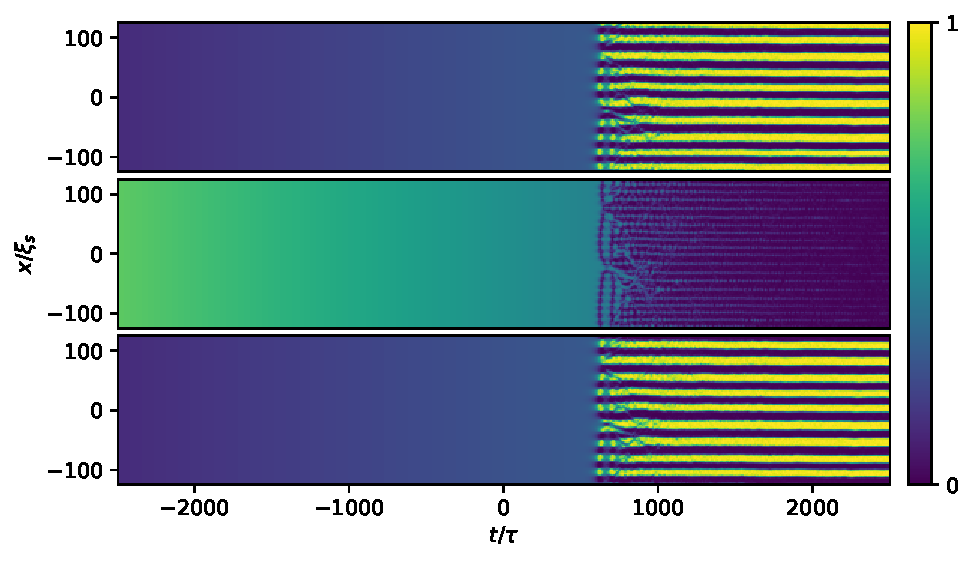
\includegraphics[width=\textwidth]{gfx/ch-spin1/BA-FM_all_densities.pdf}
    \caption[Component densities of the system as a function of time]
    {\label{fig: BA-FM-densities}
    Plots of \(|\psi_1|^2\) (top) \(|\psi_0|^2\) (middle) and
        \(|\psi_{-1}|^2\) (bottom) as a function of time for a \(256\xi_s\)
        spatial subregion of the condensate for
        \( \tau_Q=1000\tau \).
        After the critical point is passed (\(t/\tau=0\)), FM domains form in
        the \(\psi_{\pm 1}\) components, indicated by the bright density peaks.
        The location of a bright density peak in one component matches with a
        density minimum in the other component, showcasing the opposite
        spin-projection.}
\end{figure}
Fig.~\ref{fig: BA-FM-densities} shows the full evolution of the density of each
component for a quench time \( \tau_Q=1000\tau \).
As the Zeeman shift is quenched, we see the density of the \(\psi_0\) component
linearly decrease as the \(\psi_{\pm 1}\) components increase.
After the critical point at \(t/\tau=0\) is passed, there is a freeze-out time
(see Sec.~\ref{sec: the-KZM}) before the system crosses into the ferromagnetic
phase.
During this new phase, we see the formation of ferromagnetic domain walls
(characterised by the bright density peaks) in the \(\psi_{\pm 1}\) components
as the order parameter adjusts to the new ground state.
These domains are spatially separated and where there is zero density in one of
the components, there is maximal density in the other, so that overall the total
density \(n=\sum_m\psi_m^*\psi_m\) is uniform.

The KZM predicts in Eq.~\eqref{eq: KZM-domain-size} that the size of the domains
grow as the quench rate decreases.
\begin{figure}[tb]
    \centering
    \begin{subfigure}{0.49\textwidth}
        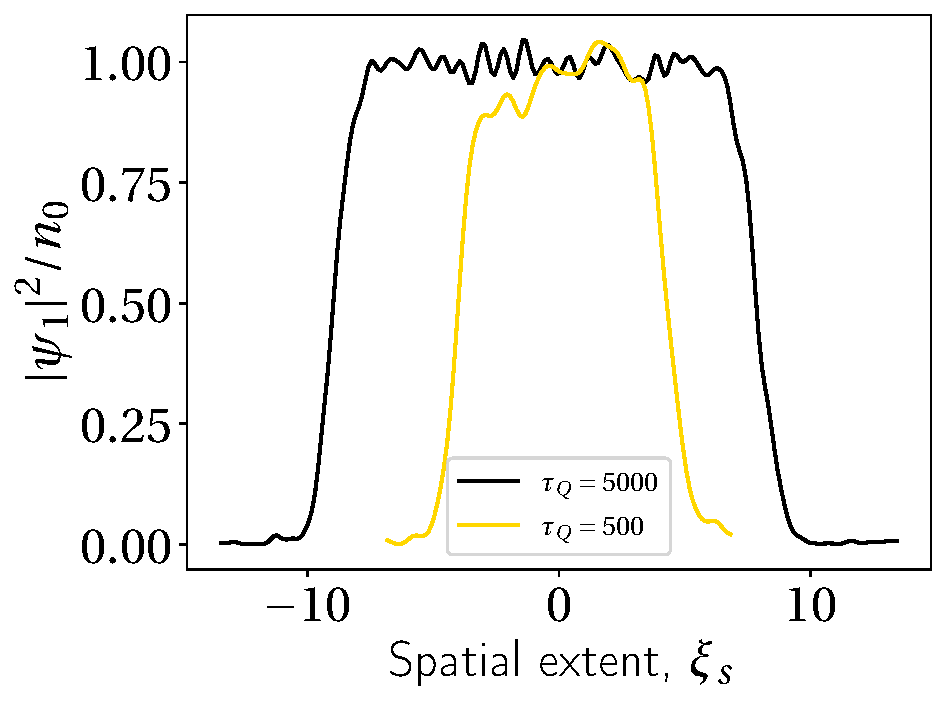
\includegraphics[width=\textwidth]{gfx/ch-spin1/BA-FM_domain_width.pdf}
        \caption{\label{fig: BA-FM-domain-width-comparison}}
    \end{subfigure}
    \begin{subfigure}{0.49\textwidth}
        \includegraphics[width=\textwidth]{gfx/ch-spin1/BA-FM_domain_onset.png}
        \caption{\label{fig: BA-FM-domain-onset}}
    \end{subfigure}
    \caption[Density profile across an average FM domain]
    {(a): Density profile of the \(\psi_1\) component across an average
        domain in a simulation with \(\tau_Q=5000\tau \) (black line) and
        \(\tau_q=500\) (gold line).
        Domain size appear proportional to the quench time \(\tau_Q\), with
        slower quenches having large domains, which supports the KZ theory
        (see Eq.~\eqref{eq: KZM-domain-size}).
        (b): Time evolution of \( |\psi_1|^2\) for a \(256\xi_s\) spatial
        subregion for \( \tau_Q=500\tau \) (top) and \(\tau_Q=1000\tau \)
        (bottom) showcasing the difference in the time it takes for domain
        formation to occur, which faster quenches leading to an earlier onset
        of domain formation when compared with slower quenches.}
\end{figure}
Fig.~\ref{fig: BA-FM-domain-width-comparison} shows the average domain size
for two different simulations with \(\tau_Q=500\) and \(\tau_Q=5000\).
We see that the quench with larger \(\tau_Q\) produces domains that have a
larger width than those of faster quenches, supporting the Kibble-Zurek theory.
In addition, we plot the time evolution of \(|\psi_1|^2\) for \(\tau_Q=500\)
and \(\tau_Q=1000\) in Fig.~\ref{fig: BA-FM-domain-onset}.
We see the ferromagnetic domain formation is delayed in the simulation
with a slower quench rate, again supporting the prediction in
Eq.~\eqref{eq: freeze-out-scaling}.

One can count the number of ferromagnetic domains in the system and see the
dependence on \( \tau_Q \).
To do this, we identified that each domain is associated with a corresponding
density peak, and subsequently developed a numerical algorithm that counts the
number of density peaks in each component and sums the result to give the total
number of domains, \(N_d\).
We calculate this quantity at the end of each simulation to ensure that the
domains are frozen and avoid the early-time coarsening taking place which could
affect the total number of domains present.
\begin{figure}[htb!]
    \centering
    \includegraphics[width=0.75\textwidth]{gfx/ch-spin1/FM_domains_scaling.pdf}
    \caption[Total ferromagnetic domains in the system versus the quench rate
        \(\tau_Q\)]
    {The number of ferromagnetic domains as a function of the
        quench time. Each point represents 50 simulations and the
        error bar gives one standard deviation. Overlaid are the scaling lines
        \(\tau_Q^{-1/3}\) (black dashed line) and \(\tau_Q^{-1/5}\)
        (red dotted line).\label{fig: FM-domains-scaling}}
\end{figure}
In Fig.~\ref{fig: FM-domains-scaling} we plot the total number of domains
as a function of the quench time, where each point represents fifty ensemble
runs for each simulation.
We find excellent agreement with the predicted value of
\(N_d \sim \tau_Q^{-1/4}\) for sufficiently fast quenches (\(\tau_Q < 2
\times 10^3\)).
However, for slower quenches, a clear deviation from the predicted scaling
occurs.
Similar deviation from the predicted KZM scaling has been observed in other
works where the quantities investigated were measured far past the critical
point~\cite{Su2013, Swislocki2013}.
The deviation observed in our system can be attributed to a crossover into a
different regime that follows the predictions of a Landau-Zener
model~\cite{Zurek2005,Damski2005, Pellegrini2008,Divakaran2008}.

\subsection{Power-law scaling near the critical point}
Since we know the relevant unstable mode within our system, we can investigate
power-law scaling near the critical point.
To begin, we start with the fluctuation operator associated with the
Bogoliubov spectrum \(E_{k, fz}\) given in Eq.~\eqref{eq: a_k-fz}.
\begin{figure}[tb]
    \centering
    \begin{subfigure}{0.45\textwidth}
        \includegraphics[width=\textwidth]
        {gfx/ch-spin1/1d_BA-FM_5000_fluctuation_diff.pdf}
        \caption{\label{fig: fluctuation-diff}}
    \end{subfigure}
    \begin{subfigure}{0.45\textwidth}
        \includegraphics[width=\textwidth]{gfx/ch-spin1/BA-FM_Qa_scaling.pdf}
        \caption{\label{fig: Q_a-scaling}}
    \end{subfigure}
    \caption[Growth of the fluctuation operator]
    {(a): The modulus of the fluctuation operator in
        Eq.~\eqref{eq: a_k-fz} for \(k=1\) and
        \(\tau_Q=5000\).
        The plot shown is obtained by averaging over all runs in the ensemble.
        (b): The critical value \(Q_a\) as a function of the quench time.
    }
\end{figure}
Fig.~\ref{fig: fluctuation-diff} shows the above quantity for a quench time
of \(\tau_Q=5000\) with \(k=1\).
The quantity remains zero until after the critical point is passed, where
a rapid period of growth occurs.
This onset of this growth corresponds to the ferromagnetic domains forming
within the system (see Fig.~\ref{fig: BA-FM-densities}).
Motivated by previous work~\cite{Damski2007, Qiu2020}, we define a time,
\( \tilde{t} \), which is the time when \(|\hat{a}_{k, {f_z}}|\) first
exceeds 1\% of its maximum value: \(|\hat{a}_{k, {f_z}}(\tilde{t})| =
0.01\times \max|\hat{a}_{k, {f_z}}(t)|\).
For the system in Fig.~\ref{fig: fluctuation-diff}, we obtain
\(\tilde{t}=598\tau \).
Using this time, we can extract the critical value of \( q \) that this growth
occurs at, \(Q(\tilde{t}) = Q_a\).
Fig.~\ref{fig: Q_a-scaling} shows \(Q_a\) as a function of the quench time.
We see a clear power-law scaling of \(Q_a \propto \tau_Q^{-\frac{1}{2}}\) for
all values of \( \tau_Q \) tested.
This exponent differs from observed results in previous works investigating
second-order phase transitions~\cite{Damski2007, Anquez2016, Swislocki2013}
where an exponent of \(-1/3\) is observed.
Our observation of a \(-1/2\) exponent signifies a deviation from
the Kibble-Zurek theory which appears to be a consequence of the properties of
the DQCP\@.

\subsection{Crossing two phase transitions}
To test the robustness of the observed scaling, we combine the effort of the
previous two numerical studies into one.
Namely, we investigate the scaling of the density of defects using a simulation
that spans two phase transitions.
Starting from the polar phase at \(Q  = 2.5\), we quench the quadratic Zeeman
shift such that we cross over to the BA phase at \(Q=2\) and finally the FM
phase at \(Q=0\).
This quench then evidently spans two phase transitions: one second-order, and
one first-order.
Our numerical set up is exactly the same as the previous section.

\begin{figure}
    \centering
    \includegraphics[width=0.75\textwidth]{gfx/ch-spin1/polar-BA-FM_domains.pdf}
    \caption{\label{fig: polar-ba-fm-defects}Number of ferromagnetic domains as
    a function of the quench time, \(\tau_Q\), after the system has crossed two
    phase transitions.
    Each point is averaged over 5 runs, with the error bars giving \(\pm 1\)
    standard deviation.}
\end{figure}
We once again count the number of ferromagnetic domains present at the end of
the simulation when the system is in the FM phase.
Results for the density of defects are plotted in
Fig.~\ref{fig: polar-ba-fm-defects}.
Despite passing through two phase transitions, we observe qualitatively similar
behaviour to that of previous transition crossing only the first-order phase
transition (see Fig.~\ref{fig: FM-domains-scaling}).
For fast quenches (\(\tau_Q \lesssim 10^3 \)), the scaling of the density of
defects follows closely to \(N_d \sim \tau_Q^{-1/4}\).
Similar to the previous case, there is a deviation from this scaling when the
quench time becomes slower (\(\tau_Q > 10^3\)).
This shows that the scaling of the density of defects for fast quenches is
robust, and is unaffected by passing through other phase transitions.

\section{Conclusions}
In this chapter we have investigated the KZM across both second-order,
continuous QPTs and first-order, discontinuous QPTs using a spin-1 BEC with
\(c_1 < 0\)as a test bed system.
We initially reproduced a known result, and showed that the KZM accurately
predicted observed scaling laws across a second-order, continuous QPT in a
spin-1 BEC between the polar and BA phases.
In particular, we measured the freeze-out time directly by measuring the time at
which the transverse magnetisation (initially zero in the polar phase) became
non-zero after crossing to the BA phase.

The primary work of this chapter consisted of analytical and numerical
investigations into a first-order, discontinuous QPT across the BA and FM
phases in a spin-1 BEC with \(c_1 < 0\).
We showed that by accounting for a gapless dispersion relation, the KZM can be
generalised to such a discontinuous QPT, which, for our spin-1 system in
question, lead to a scaling of the density of defects as
\(N_d \sim \tau_Q^{-1/4}\).
The observed scaling laws of our generalised KZM differed from those observed
across continuous quantum critical points for the same spin-1 BEC model
discussed initially.
Furthermore, by linearising the resulting spinor GPEs, we obtained scaling laws
governing the growth of the unstable excitations as the system transitions to
the FM phase.

Numerical simulations provided excellent agreement for both the short-time
growth of unstable excitations in addition to the number of FM domains formed
after the critical point was passed.
The robustness of our theory was confirmed by performing similar simulations
which crossed both a second-order QPT (polar to BA) and a first-order QPT
(BA to FM), which gave quantitatively similar results to the previously observed
scaling laws.
\chapter{Vortex connections across topological interfaces}\label{chap: spin-2}
In this chapter, we both analytically and numerically investigate the physics
of topological defects when connected across topological interfaces in spin-2
Bose-Einstein condensates.
We demonstrate that a particularly rich phenomenology of topological defects
at the coherent
interface between regions of different broken symmetries can be realised in
spin-2 Bose-Einstein condensates.
In particular, we propose that an interface between uniaxial and biaxial nematic
phases exhibiting continuous and discrete order-parameter symmetry,
respectively, can be realised using existing experimental techniques.
We construct spinor wave functions that represent topological defects connecting
across the interface.
By numerical energy relaxation as well as simulations of dynamics, we
characterise the emergence of non-trivial defect core structures.
We further demonstrate the emergence of composite vortex-core structures and
continuous connection of fractional vortices representing non-Abelian charges in
interfaces involving the cyclic and ferromagnetic phases, which could be
realised through manipulation of the inter-atomic interactions.
Our results suggest the spin-2 Bose-Einstein condensates as experimentally
accessible test beds for interface physics with all combinations of continuous
and discrete symmetries, as well as phases supporting non-Abelian defects.

\section{Introduction to topological interfaces}
When topologically distinct phases, described by different order parameters,
coexist in a continuous and coherent ordered medium, a topological interface
must form at the phase boundary, where the different broken symmetries connect
smoothly.
Such interfaces are ubiquitous across many areas of physics, from the
\(A\)--\(B\) phase boundary in superfluid
helium~\cite{Salomaa1987, Volovik2009, Finne2006}, to appearing as the
termination points of cosmic strings in theories of the early
universe~\cite{Kibble1976, Vilenkin1994}, and even in brane-inflation
models in superstring theory~\cite{Dvali1999, Sarangi2002}.
They may also play an important role for superconducting materials in
solid-state physics~\cite{Bert2011}.
The different order-parameter symmetries imply that the bulk medium on either
side of the interface supports different families of topological defects and
textures, which therefore cannot cross the interface unchanged, but must either
terminate, or connect continuously and non-trivially to an object representing
the different topology on the other side.
Due to the ubiquitous nature of topological interfaces, their study in
controlled experiments becomes of general importance, inspiring the use of
laboratory systems as emulators for interface physics in contexts otherwise not
amenable to experimental observations, for example the simulation of
brane-collision processes using superfluid \(^3\)He~\cite{Bradley2007}.

Topological-interface physics becomes especially intriguing when the medium on
either or both sides of the interface exhibits point-group order-parameter
symmetry~\cite{Xiao2022}, leading to the existence of non-Abelian defects,
whose charges depend on the presence of other defects in the system and whose
dynamics is highly constrained~\cite{Poenaru1977,Mermin1979,Kobayashi2009}.
Such fully discrete order-parameters symmetries readily arise in particular
phases of spin-2 and -3 Bose-Einstein condensates
(BECs)~\cite{Barnett2006,Barnett2007,Semenoff2007,Makela2007,Yip2007,
    Kobayashi2009,Borgh2016b,Xiao2022}, which have consequently been proposed, e.g.,
as candidates for quantum-computation applications~\cite{Mawson2019} and for
realisation of non-Abelian quantum turbulence~\cite{Mawson2015}.
Spinor BECs~\cite{Kawaguchi2012,StamperKurn2013} are constructed in all-optical
traps such that the internal spin-degrees of freedom are not frozen out by
strong magnetic fields~\cite{StamperKurn1998} and provide an ideal
testing ground for investigating interface
physics~\cite{Borgh2012,Borgh2013,Borgh2014}.
Their rich phase diagrams~\cite{Kawaguchi2012} exhibit a rich variety of
phases with different order-parameter symmetries, supporting radically different
families of topological defects, such as singular
vortices~\cite{Yip1999,Isoshima2002,
    Zhou2003,Ji2008,Takahashi2009,Lovegrove2012,Weiss2019,Xiao2021}, including
vortices carrying fractional circulation~\cite{Leonhardt2000,Ji2008,Seo2015,
    Semenoff2007,Borgh2016b,Xiao2022}, and non-singular
textures~\cite{MizushimaPRL2002, MizushimaPRA2002,
    Martikainen2002,Choi2012,Lovegrove2014},
monopoles~\cite{Pietila2009,Ollikainen2017,Ruostekoski2003,Ray2014,Ray2015,
    Mithun2022}, and even Skyrmions~\cite{Tiurev2018,Lee2018} and
knots~\cite{Hall2016}.

With spin-2 BECs being experimentally readily realisable~\cite{Schmaljohann2004}
and  experimental techniques for controlled creation of vortices with internal
point-group symmetries having recently been developed~\cite{Xiao2022}, these
systems are poised as immediate candidates for the realisation of topological
interfaces with non-Abelian defect physics. Here we analytically construct spinor
wave functions representing continuous defect connections across all
permutations of topological interfaces between the different ground-state
phases of spin-2 BECs and demonstrate their energy relaxation by numerical
simulation for illustrative examples. We have previously suggested that
topological interface could be realised in spin-1 BECs through the spatial
engineering of induced Zeeman shifts~\cite{Borgh2014} (which can also control
the defect-core symmetry properties~\cite{Borgh2016a,Underwood2020}) or, less
straightforwardly, using optical or microwave Feshbach resonances to manipulate
atomic scattering lengths~\cite{Borgh2012,Borgh2013}. Here we show how the
former technique readily lends itself to the formation of a topological
interface between uniaxial (UN) and biaxial nematic (BN) phases with commonly
used atomic species such as \({87}\)Rb. We construct solutions corresponding to
connecting singly quantized and spin vortices, as well as terminating vortices.
\textcolor{red}{[Something more here]}

\section{Interface crossing solutions in a spin-2 BEC}
As discussed in Chapter~\ref{chap: ground-states}, the spin-2 BEC gives rise to
three ground state phases in the absence of a magnetic field: Ferromagnetic,
nematic, and cyclic.
In addition to these states, additional steady-state solutions that arise in
the presence of Zeeman shifts~\cite{Kawaguchi2012}.
Here, we derive a subset of the stationary solutions that offer interpolating
solutions between different ground states.

Stationary solutions of the spin-2 GPEs are obtained by substituting
\(\psi_m = \sqrt{n}\zeta_m e^{-i\mu t/\hbar}\) into
Eqs.~\eqref{eq: spin-2-GPEs-pm2}-\eqref{eq: spin-2-GPEs-0}.
Ignoring the kinetic energy term and taking \(V(\vb{r}) = 0\), this results
in
\begin{align}
    \mu\zeta_2    & = \left(-2p + 4q + c_0n +2c_1nf_z\right)\zeta_2
    + c_1nf_-\zeta_1 + \frac{c_2}{\sqrt{5}}na_{00}\zeta^*_{-2},            \\
    \mu\zeta_1    & = \left(-p + q + c_0n +c_1nf_z\right)\zeta_1
    + c_1\left(\frac{\sqrt{6}}{2}nf_-\zeta_0 +nf_+\zeta_2\right)
    - \frac{c_2}{\sqrt{5}}na_{00}\zeta^*_{-1},                             \\
    \mu\zeta_0    & = c_0n\zeta_0 + \frac{\sqrt{6}}{2}c_1\left(nf_+\zeta_1
    + nf_-\zeta_{-1}\right) + \frac{c_2}{\sqrt{5}}na_{00}\zeta_0^*,        \\
    \mu\zeta_{-1} & = \left(p + q + c_0n - c_1nf_z\right)\zeta_{-1}
    + c_1\left(\frac{\sqrt{6}}{2}nf_+\zeta_0 +nf_-\zeta_{-2}\right)
    - \frac{c_2}{\sqrt{5}}na_{00}\zeta^*_{1},                              \\
    \mu\zeta_{-2} & = \left(2p + 4q + c_0n - 2c_1nf_z\right)\zeta_{-2}
    + c_1nf_+\zeta_{-1} + \frac{c_2}{\sqrt{5}}na_{00}\zeta^*_{2}.          \\
\end{align}

We can choose the overall phase such that \(\zeta_0\) is real.
In addition, since the system is assumed to be symmetric about the \(z\)-axis,
we can let \(f_y=0\) without loss of generality.
\textcolor{red}{Need to convince myself on this last assumption.}
We consider the specific case where the transverse magnetisation is zero
\(f_{\pm} = 0\), which is valid for \(q < 0\)
Assuming the above, the stationary equations can be transformed into the
following simplified set of equations:
\begin{align}
    0 & = (-2p + 4q + c_0n + 2c_1nf_z - \mu)\zeta_2
    + \frac{c_2}{\sqrt{5}}na_{00}\zeta^*_{-2},
    \label{eq: spin-2-stationary-zeta2}                                 \\
    0 & = (2p + 4q + c_0n - 2c_1nf_z - \mu)\zeta_{-2}
    + \frac{c_2}{\sqrt{5}}na^*_{00}\zeta_{2},
    \label{eq: spin-2-stationary-zetam2}                                \\
    0 & = (-p + q + c_0n + c_1nf_z - \mu)\zeta_1
    + \frac{c_2}{\sqrt{5}}na_{00}\zeta^*_{-1},
    \label{eq: spin-2-stationary-zeta1}                                 \\
    0 & = (p + q + c_0n - c_1nf_z - \mu)\zeta_{-1}
    + \frac{c_2}{\sqrt{5}}na^*_{00}\zeta_1,
    \label{eq: spin-2-stationary-zetam1}                                \\
    0 & = \left(c_0n + \frac{c_2}{\sqrt{5}}na_{00} - \mu\right)\zeta_0.
    \label{eq: spin-2-stationary-zeta0}
\end{align}

Noting that the above equations are decoupled in three parts, we can construct
the following matrix equations relating to
Eqs.~\eqref{eq: spin-2-stationary-zeta2}-\eqref{eq: spin-2-stationary-zetam2}
and Eqs.~\eqref{eq: spin-2-stationary-zeta1}
-~\eqref{eq: spin-2-stationary-zetam1}, respectively, as
\begin{align}
    \mqty(4q + 2\beta -\tilde{\mu} & \alpha                           \\
    \alpha^*                       & 4q - 2\beta -\tilde{\mu})
    \mqty(\zeta_2                                                     \\
    \zeta_{-2}^*)                  & = 0, \label{eq: zeta-pm2-matrix} \\
    \mqty(q + \beta -\tilde{\mu}   & -\alpha                          \\
    -\alpha^*                      & q - \beta -\tilde{\mu})
    \mqty(\zeta_1                                                     \\
    \zeta_{-1}^*)                  & = 0, \label{eq: zeta-pm1-matrix}
\end{align}
with Eq.~\eqref{eq: spin-2-stationary-zeta0} being recast as
\begin{equation}\label{eq: spin-2-stationary-zeta0-recast}
    (\alpha - \tilde{\mu})\zeta_0 = 0.
\end{equation}
Here, \(\tilde{\mu} = \mu - c_0n\), \(\alpha = c_2na_{20}/\sqrt{5}\) and
\(\beta = c_1nf_z - p\).
The stationary solutions are then classified according to the determinant of
the coefficient matrices of the above equations.
Explicitly, these are
\begin{align}
    D_2 & = {(4q-\tilde{\mu})}^2 -4\beta^2 - |\alpha|^2, \label{eq: D2}  \\
    D_1 & = {(q - \tilde{\mu})}^2 - \beta^2 - |\alpha|^2. \label{eq: D1}
\end{align}
From these determinants and Eq.~\eqref{eq: spin-2-stationary-zeta0-recast},
we can derive stationary solutions that interpolate between different ground
states of the spin-2 system.

\subsection{Ferromagnetic to biaxial nematic}
Consider the case \(D_1 \neq 0\) and \(D_2 = 0\).
If \(D_1 \neq 0\), then Eq.~\eqref{eq: D1} implies \(\zeta_1=\zeta_{-1} = 0\).
Additionally, if \(\alpha \neq \tilde{\mu}\),
then Eq.~\eqref{eq: spin-2-stationary-zeta0-recast} implies \(\zeta_0 = 0\).
\textcolor{red}{Rest of derivation here.}

The resulting stationary solution has the form
\begin{equation}\label{eq: FM-BN-interpolating-spinor}
    \zeta_\mathrm{FM-BN} = \mqty(\sqrt{\frac{1 + f_z/2}{2}} \\ 0 \\ 0 \\ 0 \\
    \sqrt{\frac{1 - f_z/2}{2}}),
\end{equation}
where \(f_z = p / [(c_1-c_2/20)n]\) gives the longitudinal magnetisation.
One can see that at \(p = \pm 2(c_1-c_2/20)n\) the above solution becomes
the ferromagnetic state with spin \(f_z = \pm 2\).
Alternatively, the solution becomes the BN state when \(p=0\).
Therefore, this spinor provides an interpolating solution between the
ferromagnetic and BN phases, which is controlled by the linear Zeeman shift,
\(p\).

Defect states that span the interface can be constructed from the steady state
solutions by applying a condensate phase \(\phi \) and spin rotation defined by
Euler angles (\(\alpha, \beta, \gamma \))
[see Eq.~\eqref{eq: spin-2-rotation-matrix}].
In this Chapter we focus only on a small subset of the possible defects present
in the spin-2 system.

We start from the interpolating spinor between the FM and BN phases in
Eq.~\eqref{eq: FM-BN-interpolating-spinor}.
The simplest vortex case to consider is that of a singular, singly quantised
vortex (SQV) on both sides of the interface.
Such a vortex is formed of a \(2\pi \) winding of the condensate phase about
the vortex core.
This winding is achieved by letting \(\phi = \varphi \), where \(\varphi \) is
the azimuthal angle about the core and letting the Euler angles be constant.
This resulting interpolating spinor then reads
\begin{equation}
    \zeta_\mathrm{FM-BN}^\mathrm{SQV} =
    \mqty(e^{i\varphi}\sqrt{\frac{1 + f_z/2}{2}} \\ 0 \\ 0 \\ 0 \\
    e^{i\varphi}\sqrt{\frac{1 - f_z/2}{2}}),
\end{equation}
where we have taken \(\alpha=\beta=\gamma=0\) for simplicity.
Despite being characterised by the same phase winding on both sides of the
interface, each SQV represents an entirely different object due to the
differing topologies on either side.

Another solution connecting different vortex states can be obtained from the
above by removing the winding from one of the \(\zeta_{\pm 2}\) components.
For example, if \(f_z\) interpolates from \(f_z=0\) to \(f_z=2\) and the winding
was removed from the \(\zeta_{-2}\) component, this solution would then connect
an SQV on the FM side to a half-quantum vortex (HQV) on the BN side.
For that same state, if the winding was instead removed from the \(\zeta_{2}\)
component, then the HQV on the BN side would continuously connect to a
vortex-free state on the FM side.

Spinor BECs support the non-dissipative flow of condensate spin, which gives
rise to vortex structures that carry a spin circulation, referred to as a spin
vortex.
Such vortices arise in all phases of the spin-2 BEC [REF].
An interpolating solution involving a spin vortex can be constructed through the
choice of \(\varphi=\gamma=0\) and \(\alpha=\varphi/2\) which results in a
singular SQV on the FM side which connecting to a BN spin vortex.
The resulting spinor reads
\begin{equation}
    \zeta_\mathrm{FM-BN}^\mathrm{SQV-SV} =
    \mqty(e^{-i\varphi}\sqrt{\frac{1 + f_z/2}{2}} \\ 0 \\ 0 \\ 0 \\
    e^{i\varphi}\sqrt{\frac{1 - f_z/2}{2}}),
\end{equation}
where we have chosen \(\beta = 0\).

As seen in Sec.~\ref{sec: vortices-spin-1}, the FM phase of a spin-1 BEC can
host a non-singular, coreless vortex that has a characteristic fountain-like
spin texture.
A coreless vortex can also be constructed in the spin-2 system following a
similar procedure and having \(\beta=\beta(\rho)\) be a monotonically increasing
function of the radial coordinate \(\rho = \sqrt{x^2 + y^2}\).
This, in addition to choosing the Euler angles
\(\phi - 2\gamma = 2\alpha = 2\varphi \) leads to the interpolating spinor
(\(\gamma=0\))
\begin{equation}\label{eq: FM-BN-coreless-DQV}
    \zeta_\mathrm{FM-BN}^\mathrm{coreless} = \mqty(
    C^4\sqrt{1+f_z/2} + S^4\sqrt{1-f_z/2} \\
    2e^{i\varphi}\left[C^3S\sqrt{1+f_z/2}
        - CS^3\sqrt{1-f_z/2}\right] \\
    e^{2i\varphi}\sqrt{6}C^2S^2\left[\sqrt{1+f_z/2}
        + \sqrt{1-f_z/2} \right] \\
    2e^{3i\varphi}\left[CS^3\sqrt{1+f_z/2}
        - C^3S\sqrt{1-f_z/2}\right] \\
    e^{4i\varphi}\left[S^4\sqrt{1+f_z/2} + C^4\sqrt{1-f_z/2} \right]
    ),
\end{equation}
where \(C \equiv \cos(\beta(\rho)/2)\) and \(S \equiv \sin(\beta(\rho)/2)\).
In the FM limit (\(f_z=2\)), one recovers the spin-2 coreless vortex given as
\begin{equation}\label{eq: FM-BN-coreless}
    \zeta^\mathrm{coreless} = \sqrt{2}\mqty(C^4 \\ 2e^{i\varphi}C^3S \\
    e^{2i\varphi}\sqrt{6}C^2S^2 \\ 2e^{3i\varphi}CS^3 \\ e^{4i\varphi}S^4
    ).
\end{equation}
The spherical harmonic representation of this vortex is plotted in
Fig.~\ref{subfig: coreless-initial}, where the characteristic fountain-like
texture becomes apparent.
The spinor in the cyclic limit (\(f_z=0\)) reads
\begin{equation}\label{eq: FM-BN-DQV}
    \zeta^\mathrm{DQV} = \mqty(
    C^4 + S^4 \\
    2e^{i\varphi}CS\left[C^2-S^2\right] \\
    2e^{2i\varphi}\sqrt{6}C^2S^2 \\
    2e^{3i\varphi}CS\left[S^2 - C^2\right] \\
    e^{4i\varphi}\left[C^4 + S^4\right]).
\end{equation}
It is not immediately obvious from the form of the spinor the type of vortex
present on the cyclic side of the interface.
To investigate the vortex state, we plot the spherical harmonics of the state
defined in Eq.~\eqref{eq: FM-BN-DQV} in
Fig.~\ref{subfig: DQV-initial}.
\begin{figure}
    \centering
    \begin{subfigure}{0.45\textwidth}
        \includegraphics[width=\textwidth]
        {gfx/ch-spin2/C-FM=2_coreless_FM_init_spherical.pdf}
        \caption{\label{subfig: coreless-initial}}
    \end{subfigure}
    \begin{subfigure}{0.45\textwidth}
        \includegraphics[width=\textwidth]
        {gfx/ch-spin2/C-FM=2_coreless_cyclic_init_spherical.pdf}
        \caption{\label{subfig: DQV-initial}}
    \end{subfigure}
    \caption{\label{fig: coreless-doubly-quantised} Spherical harmonic
        representation of the vortex configurations on each side of the FM-BN
        interface defined in Eq.~\eqref{eq: FM-BN-coreless-DQV}.
        (a): Spin-2 FM coreless vortex given by Eq.~\eqref{eq: FM-BN-coreless}.
        (b): Doubly quantised vortex on the BN side of the interface, given by
        Eq.~\eqref{eq: FM-BN-DQV}.
        \textcolor{red}{Current DQV is for cyclic case, update to BN.}}
\end{figure}
By tracing a point about the vortex line, the phase changes by a total of
\(4\pi \) indicating a doubly quantised vortex.

\subsection{Uniaxial nematic to biaxial nematic}
Consider \(D_1 \neq 0\) and \(D_2 = 0\), then \(\zeta_1 = \zeta_{-1} = 0\).
Furthermore, if \(\tilde{\mu} = \alpha \), then all of \(\zeta_{\pm 2}\) and
\(\zeta_0\) can be non-zero.
\textcolor{red}{Rest of derivation here.}

The final solution reads
\begin{equation}\label{eq: UN-BN-interpolating-spinor}
    \zeta_\mathrm{UN-BN} = \mqty(
    \frac{\sqrt{1 - \eta}}{2} \\
    0 \\
    \sqrt{\frac{1 + \eta}{2}} \\
    0 \\
    \frac{\sqrt{1 - \eta}}{2}
    ),
\end{equation}
where \(\eta = 10q /|c_2|n \in [-1, 1]\).
This solution depends only on the quadratic Zeeman shift, which can alter the
spinor between phases.
When \(q = c_2n / 10\) the system is in the uniaxial nematic phase.
In the opposite limit when \(q = -c_2n/10\) the system is in the biaxial
nematic phase.
This spinor therefore provides interpolating solutions between the uniaxial
nematic and biaxial nematic phases, engineered through manipulation of the
quadratic Zeeman shift.

To determine the stability of this interpolating spinor, we compare the energy
per particle given by~\cite{Kawaguchi2012}
\begin{equation}
    E_\mathrm{part} = \sum_{m=-2}^{2}(-pm + qm^2)|\zeta_m|^2 + \frac{c_0n}{2}
    + \frac{c_1n}{2}|\vb{f}|^2 + \frac{c_2n}{2}|a_{00}|^2.
\end{equation}
The energy of the interpolating spinor given in
Eq.~\eqref{eq: UN-BN-interpolating-spinor} reads
\(E^\mathrm{UN-BN}_\mathrm{part} = 2q + c_0n/2 - 10q^2/c_2n\)
\textcolor{red}{Messy notation}.
Comparing this energy with that of the UN phase
\(E^\mathrm{UN}_\mathrm{part} = (c_0+c_2/5)n/2\) reveals that this interface is
stable for \(|q| \leq |c_2|n/10\).

The consequence of a spatially-dependent \(\eta \) is revealed from the spin
singlet-duo and -trio amplitudes.
Upon substitution of Eq.~\eqref{eq: UN-BN-interpolating-spinor} into
\textcolor{red}{Define duo and trio amplitudes, more than likely in theory
    chapter} yields
\begin{equation}
    \begin{aligned}
        |A_{20}|^2 & = \frac{1}{10} \left[(\eta^2-1)\cos\theta
        + \eta^2 + 1\right],                                          \\
        |A_{30}|^2 & = \frac{1+\eta}{4} \left[3\left(\eta ^2-1\right)
            \cos\theta
            + \eta(5 \eta -8) + 5\right],
    \end{aligned}
\end{equation}
where \(\theta = \chi_2 + \chi_{-2} - 2\chi_0\) and \(\chi_j = Arg(\psi_j)\) for
component \(j=-2, 0, 2\).
We plot both the singlet-duo and -trio amplitudes in
Fig.~\ref{fig: UN-BN-duo-trio} in a parameter space of \((\eta, \theta)\).
\begin{figure}
    \centering
    \includegraphics[width=0.75\textwidth]{gfx/ch-spin2/a20-a30-varying.png}
    \caption{\label{fig: UN-BN-duo-trio} Spin singlet-duo (left) and -trio
        (right) amplitudes for the interpolating spinor in
        Eq.~\eqref{eq: UN-BN-interpolating-spinor}.
        Due to the spatially-dependent \(\eta \), this spinor continuously
        interpolates between the UN, BN, and cyclic phases depending on the
        relative phase difference between the components.}
\end{figure}
We see that this spinor interpolates between the different phases of UN, BN and
cyclic depending on both \(\eta \) and the relative phase difference
\(\theta \).
For example, if one were to maintain \(\theta=0\) and interpolate \(\eta \),
then there would be multiple transitions between the UN (\(|a_{00}|^2 = 1\)) and
BN (\(|a_{00}|^2 = 0\)) phases.
As we shall see in the numerical investigation of such an interface, this has
profound effects on the structure of topological defects connecting across
the interface.

From the interpolating spinor in Eq.~\eqref{eq: UN-BN-interpolating-spinor} we
can construct various topological defect crossing solutions.
The simplest case is the connection of SQVs on either side of the interface.
Such a connection is realised by the choice \(\phi = \varphi \) whilst keeping
the Euler angles constant.
A representative example with \(\alpha = \gamma = 0\) is given by
\begin{equation}
    \zeta^\mathrm{SQV}_\mathrm{UN-BN} =
    \frac{e^{i\varphi}}{8}\begin{pmatrix}
        \sqrt{6} D_+ \sin ^2\beta _0 + 2D_- \left(\cos^2\beta _0+1\right) \\
        -2 \left(D_--\sqrt{3} D_+\right) \sin 2 \beta _0                  \\
        \sqrt{2}\left[ \sqrt{3} D_- \sin ^2\beta _0 -2D_+
        \left(1-3 \cos^2 \beta _0\right)\right]                           \\
        2 \left(D_--\sqrt{3} D_+\right) \sin 2 \beta _0                   \\
        \sqrt{6} D_+ \sin ^2\beta _0+D_- \left(\cos^2\beta _0+1\right)
    \end{pmatrix},
    \label{eq: UN-BN-SQV-SQV}
\end{equation}
where \(D_{\pm} = \sqrt{1 \pm \eta}\) and \(\beta=\beta_0\) is an arbitrary
constant.
The explicit form of the above equation in the UN
(\(D_+ = \sqrt{2}, D_- = 0\)) and BN (\(D_0 = 0, D_- = \sqrt{2}\)) limits
is given, respectively, as
\begin{equation}
    \zeta_\mathrm{UN}^\mathrm{SQV} =  \frac{e^{i\varphi}}{4}\mqty(
    \sqrt{3}\sin^2\beta_0 \\
    \sqrt{6}\sin2\beta_0 \\
    -2(1 - 3\cos^2\beta_0) \\
    -\sqrt{6}\sin2\beta_0 \\
    \sqrt{3}\sin^2\beta_0
    ), \qquad
    \zeta_\mathrm{BN}^\mathrm{SQV} =  \frac{e^{i\varphi}}{4}\mqty(
    \sqrt{2}(\cos^2\beta_0 + 1) \\
    -\sqrt{2}\sin2\beta_0 \\
    2\sqrt{3}\sin^2\beta_0 \\
    \sqrt{2}\sin2\beta_0 \\
    \sqrt{2}(\cos^2\beta_0 + 1)
    ).
\end{equation}
One can see that upon the substitution of \(\beta_0 = 0\) in the above spinors,
we recover the SQV case in both the UN
\(\zeta^\mathrm{SQV} = {(0,0,e^{i\varphi},0,0)}^T\) and BN
\(\zeta^\mathrm{SQV} = {(e^{i\varphi},0,0,0,e^{i\varphi})}^T/\sqrt{2}\) limits.
It is important to note that, despite being characterised by the same phase
winding, the SQVs on either side of the interface represent entirely different
objects due to the differing topologies of the UN and BN phases.

Spin vortices can be connected across the interface by choosing
\(\alpha=\varphi, \beta=\beta_0 \) and \(\phi = \gamma = 0\), resulting in the
spinor
\begin{equation}\label{eq: UN-BN-SV-SV-spinor}
    \zeta^\mathrm{SV} =
    \frac{1}{8}\begin{pmatrix}
        e^{-2i\varphi}\left[\sqrt{6} D_+ \sin ^2\beta _0
        + 2D_- \left(\cos^2\beta _0+1\right)\right]                   \\
        -2e^{-i\varphi} \left(D_--\sqrt{3} D_+\right) \sin 2 \beta _0 \\
        \sqrt{2}\left[ \sqrt{3} D_- \sin ^2\beta _0
        - 2D_+ \left(1-3 \cos^2 \beta _0\right)\right]                \\
        2 e^{i\varphi}\left(D_--\sqrt{3} D_+\right) \sin 2 \beta _0   \\
        e^{2i\varphi}\left[\sqrt{6} D_+ \sin ^2\beta _0
            + 2D_- \left(\cos^2\beta _0+1\right)\right]
    \end{pmatrix}.
\end{equation}
In particular, spin vortices arise in both components for
\(\beta_0 \neq 0, \pi \), where the spin vortex in each phase carries opposite
the spin winding of the other spin vortex.
For the specific cases of \(\beta_0 = 0, \pi \),
Eq.~\eqref{eq: UN-BN-SV-SV-spinor} instead results in a spin vortex in the BN
phase that continuously connects to a vortex-free state in the UN limit.

In addition to line defects, i.e., vortices, it is also possible to construct
point defects that terminate at the topological interface.
The possibility in the UN-BN interface is that of a monopole, which is
characterised by a spherically symmetric dependence of the nematic axis
\(\vb{\hat{d}} = (\cos\varphi \sin\theta, \sin\varphi \sin\theta, \cos\theta)\),
where \(\theta \) is the polar angle in spherical coordinates.
The monopole solution is derived from Eq.~\eqref{eq: UN-BN-interpolating-spinor}
using the substitution \(\beta = \theta \) and \(\alpha=\varphi \).
\textcolor{red}{Would quite like an image of the initial state somehow.}


\subsection{Cyclic to nematic}
A steady-state solution that interpolates between the nematic and cyclic phases
can be found by including phase coefficients in
Eq.~\eqref{eq: UN-BN-interpolating-spinor}, namely
\begin{equation}\label{eq: C-N-interpolating-spinor}
    \zeta^\mathrm{C-N} = \mqty(
    e^{i\chi_2}\frac{\sqrt{1 + \eta}}{2} \\
    0 \\
    e^{i\chi_0}\sqrt{\frac{1 - \eta}{2}} \\
    0 \\
    e^{i\chi_{-2}}\frac{\sqrt{1 + \eta}}{2}),
\end{equation}
where \(\eta = 10q/(|c_2|n)\).
The quadratic Zeeman shift can be used to interpolate the above solution between
the different phases.
At \(q = 0\) the above solution becomes the three component cyclic
\(\zeta_\mathrm{C} = {(1, 0, i\sqrt{2}, 0, 1)}^T/2\).
The sign of the quadratic Zeeman shift determines which nematic state is chosen.
If \(q = -c_2n/10\) then the solution becomes biaxial nematic
\(\zeta_\mathrm{BN} = {(1, 0, 0, 0, 1)}^T/\sqrt{2}\).
In the opposite limit of \(q = c_2n/10\) then the system is in the uniaxial
nematic state \(\zeta_\mathrm{UN} = {(0, 0, 1, 0, 0)}^T\).

\subsection{Cyclic to ferromagnetic}
An additional stationary solution can be found by considering \(D_1=D_2=0\).
Eq.~\eqref{eq: D2} and Eq.~\eqref{eq: D1} can then be solved exactly, to yield
\begin{equation}
    \tilde{\mu} = \pm \sqrt{4q^2 + |\alpha|^2}.
\end{equation}
If \(q \neq 0\), then \(\tilde{\mu} \neq \alpha \) which implies \(\zeta_0=0\)
from Eq.~\eqref{eq: spin-2-stationary-zeta0-recast}.
Zero transverse magnetisation then implies we have
\(0 = 2c_1n(\zeta_2^*\zeta_{1} + \zeta_{-1}^*\zeta_{-2})\).
\textcolor{red}{Rest of derivation here.}

The final solution reads
\begin{equation}
    \zeta^\mathrm{C-FM} = \mqty(\sqrt{\frac{1 + f_z}{3}} \\ 0 \\ 0 \\
    \sqrt{\frac{2 - f_z}{3}} \\ 0),
\end{equation}
where \(f_z = (p - q) / (c_1n)\).
At zero magnetisation, \(f_z = 0\), this solution is precisely the two-component
cyclic state.
The solution also interpolates between different ferromagnetic states depending
on the magnetisation.
If \(f_z = -1\) one recovers an FM-1 solution.
Conversely, \(f_z = 2\) yields the FM-2 solution.
This spinor there provides an interpolating solution between the cyclic and
ferromagnetic phases.

\section{Dynamical stability of interface solutions}

\section{Numerical investigations of defect crossing physics}
\subsection{Uniaxial nematic to biaxial nematic interface}
\subsection{Cyclic to ferromagnetic interface}
\subsection{Cyclic to biaxial nematic interface}

\chapter{Conclusions \& future work}\label{chap: conclusions}
In this thesis we have investigated a variety of topics in spinor and
pseudospinor condensates.
In particular, we investigated the relaxation dynamics of half-quantum vortices
in a pseudospin-1/2 system, a generalised Kibble-Zurek scaling in a spin-1
system, and finally topological interface dynamics in a spin-2 system.

Chapters 2 and 3 introduced the necessary mathematical framework needed to
understand these systems in detail.
We provided detailed constructions of the resulting interaction Hamiltonians for
each of these systems, with a focus on the differences arising.
Furthermore, chapter 3 introduced novel vortex structures encountered in spinor
BECs and how to construct them using spin rotations.

Chapter 4 investigated the relaxation dynamics of half-quantum vortices (HQVs)
in a pseudospin-1/2 system.
We presented a method of constructing an initially turbulent system of \(48^2\)
HQVs using previous numerical work for a scalar system~\cite{Billam2014}.
We then described our method of investigating the relaxation process of the
system by varying the ratio of inter-species and intra-species interactions,
\(\gamma \).
A minor result of the study showed that, despite carrying half the circulation,
the kinetic energy spectrum revealed similarities to that of scalar vortices.
The major result of the study was identifying anomalous scaling laws of the
vortex number that occurred when \(\gamma \gtrsim 0.6\).
In particular, for values of \(\gamma < 0.6\), there was a uniform \(t^{-2/5}\)
scaling of the vortex number throughout the simulations.
However, as \(\gamma \) was increased past this point, a shoulder started to
develop, separating the relaxation dynamics into two distinct parts.
A larger \(\gamma \) led to a steeper decay rate of the vortices at early times,
with the largest \(\gamma \) \((\gamma = 0.9)\) achieving a \(t^{-3/2}\) decay
rate.
At later times the anomalous scaling reverted to the observed \(t^{-2/5}\)
scaling.
We identified the cause of the anomalous scaling by referring to previous works
investigating the inter-vortex forces~\cite{Eto2011, Kasamatsu2016}.
The larger \(\gamma \) increased the core sizes of the vortices, which in turn
meant that the inter-vortex separation was smaller.
This then meant that a new, attractive force otherwise unseen in scalar
vortices dominated, and caused the HQVs to move together and annihilate,
leading to the anomalous scaling.

In chapter 5 we investigated the Kibble-Zurek mechanism across a first-order
phase transition in a spin-1 BEC\@.
In particular, we started from the broken-axisymmetry phase of a condensate with
ferromagnetic interactions, then proceeded to quench the quadratic Zeeman shift,
\(q\), which caused the ground state of the condensate to become ferromagnetic.
Firstly, we analytically constructed scaling laws using a modified Kibble-Zurek
mechanism that accounted for our discontinuous phase transition, using theory
developed for a discontinuous critical point~\cite{Suzuki2015}.
This led to a prediction of the scaling of the density of defects as
\(\tau_Q^{-1/4}\), where \(\tau_Q\) is the quench rate, which is noticeably
different from the traditional scaling of \(\tau_Q^{-1/3}\) seen across
second-order transitions~\cite{Damski2007, Anquez2016}.
In addition, we analytically derived the scaling properties near the critical
point, which came out to be \(\tau_Q^{-1/2}\).
We then carried out numerical investigations of this phase transition.
The numerics confirmed the formation of ferromagnetic domains in the system
after the critical point of \(q_c=0\) was crossed.
The size of these domains was indeed confirmed to depend on the quench rate,
\(\tau_Q\).
Using the simulations, we then calculated the total number of ferromagnetic
domains in the system at the end of the simulation for each quench rate tested.
We found that for sufficiently slow quenches (\(\tau_Q \lesssim 2\times 10^3\))
the scaling of the defect density obeyed the predicted \(\tau_Q^{-1/4}\)
scaling.
However, at faster quench rates this scaling broke down, and instead approached
a scaling close to \(\tau_Q^{-1/5}\).
\textcolor{red}{We revealed that this phenomenon is due to\ldots}
The scaling near the critical point was also calculated, and agreed perfectly
with our predicted scaling of \(\tau_Q^{-1/2}\).
Finally, we also tested our predicted scaling laws in a system that crossed
two phase transitions, i.e., going through the polar to broken-axisymmetry to
the FM phases.
Despite passing through two phase transitions, with one of them being
second-order, the scaling of the defect density at late times was qualitatively
similar to that observed just crossing one phase transition.

Chapter 6 was concerned with investigating topological interfaces in spin-2
BECs.
We derive stationary solutions of the spin-2 Gross-Pitaevskii equations that
provided interpolating solutions between different ground state manifolds.
We then discussed the energetic stability of each of the interfaces, and how
they can be manipulated with both linear and quadratic Zeeman shifts.
From here, we progressed into a discussion regarding the connection of
topological defects across such interfaces.
Numerous types of defects were considered ranging from singly quantised
vortices (SQVs), spin vortices, fractional vortices, coreless vortices, and even
monopole point defects.
The remainder of the chapter presented numerical work investigating different
interfaces and interesting vortex connections across them.
In a uniaxial-nematic to biaxial-nematic (UN-BN) interface we showed that SQVs
initially connected across the interface spatially separate.
After doing so, composite core structures develop which are filled with a
variety of different phases.
In addition, we showed that a SQV in the BN phase connected to a vortex free
state in the UN phase would split into HQVs.
A monopole point defect was also constructed on the UN side of the interface,
which smoothly terminated on a singly quantised spin vortex line in the BN
phase.
Finally, we investigated both fractional and coreless vortices across a cyclic
to ferromagnetic (C-FM) interface.
In particular, we observed a SQV on the FM side smoothly connecting to a
third vortex on the cyclic side of the interface.
The \(\spinmag=1\) core of the third vortex extended through the FM region,
which was topologically protected by having a cyclic shell encapsulating the
vortex core.
The coreless vortex on the FM side was revealed to connect to a doubly quantised
vortex (DQV) line in the cyclic region.
Numerical results showed complex splitting behaviour from this connection.
In particular, the initial DQV on the cyclic side split into four third
vortices alongside a central two-third vortex.
On the FM side, the coreless vortex is observed to split into four singular
vortex structures.

\section{Future work}

\subsection{Two-component system}
Our numerical investigation of the relaxation dynamics of HQVs revealed
interesting behaviour unseen in similar relaxation studies involving scalar
condensates~\cite{Karl2017}.
In particular, a clear attractive force between the vortices dominates at
sufficiently high \(\gamma \), so a logical next step is to determine the cause
of this attractive force.
In fact, recently theoretical work has shed more light on the
topic~\cite{Richaud2022}.
They showed that the atoms filling the large cores of the HQVs act as a pinning
potential, driving the HQVs to collide.
This work therefore explains previously observed numerical simulations of HQV
dynamics in these systems~\cite{Eto2011, Kasamatsu2016}, and provides a
better insight into our observed decay laws.

In addition, experimental work has already been conducted investigating the
relaxation dynamics of HQVs in a spin-1 BEC~\cite{Seo2016}.
However, corresponding numerical investigations of the decay rate of the
vortices has not been carried out, and it would indeed be interesting to see
whether there is overlap with our pseudospin-1/2 work.

\subsection{Spin-1 Kibble-Zurek}
A natural extension of this work would be to a spin-2 system, which contains
further second-order and first-order phase transitions.
For example, a prime candidate for a first-order transition would be between the
nematic and ferromagnetic regimes, which could be achieved similarly to our
current work by quenching the magnetic field.

\textcolor{red}{What else?}

\subsection{Spin-2 interface problems}
Naturally, there are numerous other topological defect connections one can
extend from our current work.
However, a more beneficial direction may be in trying to recreate the
topological interfaces created in both our work and previous spin-1
work~\cite{Borgh2012, Borgh2013, Borgh2014}, which so far has remained elusive.

\textcolor{red}{What else?}


\part{Appendices}
\appendix
\chapter{Numerical techniques}\label{appendix: numerical-techniques}

\section{\label{sec: two-comp-dimensionless}Dimensionless two-component
Gross-Pitaevskii equations}

As mentioned in Sec~\ref{sec: dimensionless-equations}, dimensionless equations
offer numerous benefits, including increased numerical stability and the ease
of reformulating calculations into a desired scale and parameter regime.
Here we derive the dimensionless two-component GPEs which are stated in
Eq.~\eqref{eq: dimensionless-two-comp-GPEs}.

To begin we start with the full 3D dimensional GPEs for a two-component system:
\begin{align} \label{eq: two-comp-GPE-psi1}
    i\hbar\pdv{\psi_1}{t} &= \left(-\frac{\hbar^2\nabla^2}{2m_1} + g_1|\psi_1|^2
    +g_{12}|\psi_2|^2\right)\psi_1, \\
    i\hbar\pdv{\psi_2}{t} &= \left(-\frac{\hbar^2\nabla^2}{2m_2} + g_2|\psi_2|^2
    +g_{12}|\psi_1|^2\right)\psi_2. \label{eq: two-comp-GPE-psi2}
\end{align}
Our simulations are performed on space-time grid lattices with a spatial side
length of \(L = N_s a_s\), where \(a_s\) is the lattice spacing and the total
number of grid points is given as \(N_s^d\) where \(d\) is the dimensionality of
the system.
With these, we make use of the following dimensionless variables
\begin{align}
    \tilde{\vb{r}} = \frac{\vb{r}}{a_s}, \quad
    \tilde{g}_j = \frac{2mg_j{a_s}^{2-d}}{\hbar^2}, \quad
    \tilde{t} = \frac{t\hbar}{2ma_s^2}, \quad
    \tilde{\psi}_j = \sqrt{a_s^d}e^{2i\tilde{t}}\psi_j,
\end{align}
where \(m = m_1 = m_2\).
Using the above dimensionless quantities, we can rescale the dimensional
variables in Eqs~\eqref{eq: two-comp-GPE-psi1} -~\eqref{eq: two-comp-GPE-psi2},
which leads to the dimensionless equations
\begin{align}
    i\pdv{\tilde{\psi}_1}{t} &= \left(-\tilde{\nabla}^2
    + \tilde{g}_1|\tilde{\psi}_1|^2 + \tilde{g}_{12}|\tilde{\psi}_2|^2\right)
    \tilde{\psi}_1, \\
    i\pdv{\tilde{\psi}_2}{t} &= \left(-\tilde{\nabla}^2
    + \tilde{g}_2|\tilde{\psi}_2|^2 + \tilde{g}_{12}|\tilde{\psi}_1|^2\right)
    \tilde{\psi}_2.
\end{align}
Now, if we have atomic species where \(g_1=g_2=g\), then the above equations
simplify to (dropping the tildes for notational convenience)
\begin{align}
    i\pdv{{\psi}_1}{t} &= \left(-{\nabla}^2
    + {g}|{\psi}_1|^2 + {\gamma}|{\psi}_2|^2\right)
    {\psi}_1, \\
    i\pdv{{\psi}_2}{t} &= \left(-{\nabla}^2
    + {g}|{\psi}_2|^2 + \gamma|{\psi}_1|^2\right)
    {\psi}_2,
\end{align}
where \(\gamma = g_{12}/g\) is the ratio of inter- to intra-species interaction.

\section{\label{sec: symplectic-integrators}Symplectic integrators for spinor
Bose-Einstein condensates}
The numerics of Chapters~\ref{chap: spin-1} and~\ref{chap: spin-2} are based on
second-order symplectic integrators: a type of numerical scheme for Hamiltonian
systems.
In particular, we make use of the work of Symes \textit{et al.} for both our
spin-1~\cite{Symes2016} and spin-2~\cite{Symes2017a} systems.
Symplectic integration schemes provide highly accurate solutions for Hamiltonian
systems over extended periods of time, making them ideal for studying the
long-time dynamics in Chapter~\ref{chap: spin-1}.
In addition, the second-order numerical schemes devised by Symes \textit{et al.}
have been shown to be both simpler and more efficient than other second-order
composition methods~\cite{Wang2007}, which is critical for compute-heavy 3D
simulations as in Chapter~\ref{chap: spin-2}.

The spinor symplectic integration schemes work by splitting the spinor GPEs into
two subsystems.
The first is a single-particle-like subsystem, which includes the kinetic energy
and the Zeeman terms of the Hamiltonian, which is solved exactly in Fourier
Space.
The second system comprises the non-linear subsystem, which includes the
remaining non-linear terms in the spinor GPEs.
Due to the nature of the splitting, this remaining subsystem becomes exactly
solvable in position space.
Note that the Zeeman terms are assumed to be spatially-uniform (a good
approximation in experiments), which allows them to be included in the
single-particle-like subsystem.
However, if the Zeeman shifts are not spatially-uniform they must instead be
included with the non-linear subsystem, which still leads to analytical
solutions in the form of Jacobi elliptic functions (see
Refs.~\cite{Symes2016, Symes2017a} for details).
Finally, though not used in this thesis, the two-way splitting implies that
the scheme can be extended using the composition method of Blanes and
Moan~\cite{Blanes2002} to fourth-order, should a higher-order symplectic scheme
be required.

The numerical methods throughout this thesis have been implemented using the
personally-developed Python package
\href{https://github.com/wheelerMT/pygpe}{
    \textit{PyGPE}
}~\cite{Wheeler_PyGPE_2024}: a CUDA-accelerated library for numerically solving
the GPEs for scalar, two-component, spin-1, and spin-2 BEC systems.
It supports 1D, 2D, and 3D grid lattices, as well as possessing the ability to
run on both CPUs or Nvidia-native GPUs.
In addition, it provides tools for data handling, as well as a suite of
diagnostics functions useful for handling data from BEC simulations.

\chapter{Derivation of stationary solutions in a spin-2 Bose-Einstein
  condensate}\label{appendix: stationary}
\section{Time-independent spin-2 Gross-Pitaevskii equations}
Here we derive stationary solutions to the spin-2 GPEs that provide the
interpolating spinor wave functions that are used throughout
Chapter~\ref{chap: spin-2}.
Firstly, recall that the stationary solutions of the spin-2 GPEs are obtained by
substituting \(\psi_m = \sqrt{n}\zeta_m e^{-i\mu t/\hbar}\) into
Eqs.~\eqref{eq: spin-2-GPEs-pm2}-\eqref{eq: spin-2-GPEs-0}.
Assuming a uniform system with \(V(\vb{r}) = 0\), this results in
\begin{align}
    \mu\zeta_2 & = \left(-2p + 4q + c_0n
    + 2c_1n\langle\hat{F}_z\rangle\right)\zeta_2
    + c_1n\langle\hat{F}_-\rangle\zeta_1
    + \frac{c_2}{\sqrt{5}}nA_{00}\zeta^*_{-2}, \\
    \mu\zeta_1 & = \left(-p + q + c_0n
    + c_1n\langle\hat{F}_z\rangle\right)\zeta_1
    + c_1\left(\frac{\sqrt{6}}{2}n\langle\hat{F}_-\rangle\zeta_0
    +n\langle\hat{F}_+\rangle\zeta_2\right)
    - \frac{c_2}{\sqrt{5}}nA_{00}\zeta^*_{-1}, \\
    \mu\zeta_0 & = c_0n\zeta_0 + \frac{\sqrt{6}}{2}c_1\left(
        n\langle\hat{F}_+\rangle\zeta_1 + n\langle\hat{F}_-\rangle\zeta_{-1}
    \right) + \frac{c_2}{\sqrt{5}}nA_{00}\zeta_0^*,        \\
    \mu\zeta_{-1} & = \left(p + q + c_0n
    - c_1n\langle\hat{F}_z\rangle\right)\zeta_{-1}
    + c_1\left(\frac{\sqrt{6}}{2}n\langle\hat{F}_+\rangle\zeta_0
    +n\langle\hat{F}_-\rangle\zeta_{-2}\right)
    - \frac{c_2}{\sqrt{5}}nA_{00}\zeta^*_{1}, \\
    \mu\zeta_{-2} & = \left(2p + 4q + c_0n
    - 2c_1n\langle\hat{F}_z\rangle\right)\zeta_{-2}
    + c_1n\langle\hat{F}_+\rangle\zeta_{-1}
    + \frac{c_2}{\sqrt{5}}nA_{00}\zeta^*_{2}.
\end{align}
Follow the literature of Ref.~\cite{Kawaguchi2012}, we make the following
assumptions.
We can choose the overall phase such that \(\zeta_0\) is real and, since the
system has \(\text{SO}(2)\) symmetry about the direction of the applied magnetic
field (which we take to be the \(z\)-axis), we choose the coordinate system such
that \(\langle\hat{F}_y\rangle=0\) without loss of generality, implying
\(\langle\hat{F}_+\rangle = \langle\hat{F}_-\rangle\).
In addition, to simplify further, we consider the specific case where the
transverse magnetisation is zero \(\langle\hat{F}_{\pm}\rangle = 0\) which is
valid in a system where \(q < 0\) such that the system favours atoms in the
outer components [see Eq.~\eqref{eq: spin-2-spin-vectors}].
Assuming the above, the stationary equations can be transformed into the
following simplified set of equations:
\begin{align}
    0 & = (-2p + 4q + c_0n + 2c_1n\langle\hat{F}_z\rangle - \mu)\zeta_2
    + \frac{c_2}{\sqrt{5}}nA_{00}\zeta^*_{-2},
    \label{eq: spin-2-stationary-zeta2}                                 \\
    0 & = (2p + 4q + c_0n - 2c_1n\langle\hat{F}_z\rangle - \mu)\zeta_{-2}
    + \frac{c_2}{\sqrt{5}}nA^*_{00}\zeta_{2},
    \label{eq: spin-2-stationary-zetam2}                                \\
    0 & = (-p + q + c_0n + c_1n\langle\hat{F}_z\rangle - \mu)\zeta_1
    + \frac{c_2}{\sqrt{5}}nA_{00}\zeta^*_{-1},
    \label{eq: spin-2-stationary-zeta1}                                 \\
    0 & = (p + q + c_0n - c_1n\langle\hat{F}_z\rangle - \mu)\zeta_{-1}
    + \frac{c_2}{\sqrt{5}}nA^*_{00}\zeta_1,
    \label{eq: spin-2-stationary-zetam1}                                \\
    0 & = \left(c_0n + \frac{c_2}{\sqrt{5}}nA_{00} - \mu\right)\zeta_0.
    \label{eq: spin-2-stationary-zeta0}
\end{align}
Noting that the above equations are decoupled in three parts, we can construct
the following matrix equations relating to
Eqs.~\eqref{eq: spin-2-stationary-zeta2}-\eqref{eq: spin-2-stationary-zetam2}
and Eqs.~\eqref{eq: spin-2-stationary-zeta1}
-~\eqref{eq: spin-2-stationary-zetam1}, respectively, as
\begin{align}
    \mqty(4q + 2\tilde{\beta} -\tilde{\mu} & \tilde{\alpha} \\
    \tilde{\alpha}^*               & 4q - 2\tilde{\beta} -\tilde{\mu})
    \mqty(\zeta_2                                                      \\
    \zeta_{-2}^*)                  & = 0, \label{eq: zeta-pm2-matrix}  \\
    \mqty(q + \tilde{\beta} -\tilde{\mu}   & -\tilde{\alpha} \\
    -\tilde{\alpha}^*              & q - \tilde{\beta} -\tilde{\mu})
    \mqty(\zeta_1                                                      \\
    \zeta_{-1}^*)                  & = 0, \label{eq: zeta-pm1-matrix}
\end{align}
with Eq.~\eqref{eq: spin-2-stationary-zeta0} being recast as
\begin{equation}\label{eq: spin-2-stationary-zeta0-recast}
    (\tilde{\alpha} - \tilde{\mu})\zeta_0 = 0,
\end{equation}
where \(\tilde{\mu} = \mu - c_0n\), \(\tilde{\alpha} = c_2nA_{00}/\sqrt{5}\) and
\(\tilde{\beta} = c_1n\langle\hat{F}_z\rangle - p\).
The stationary solutions are then classified according to the determinant of
the coefficient matrices of the above equations.
Explicitly, these are
\begin{align}
    D_2 & = {(4q-\tilde{\mu})}^2 -4\tilde{\beta}^2 - |\tilde{\alpha}|^2,
    \label{eq: D2}                                                        \\
    D_1 & = {(q - \tilde{\mu})}^2 - \tilde{\beta}^2 - |\tilde{\alpha}|^2.
    \label{eq: D1}
\end{align}
From these determinants and Eq.~\eqref{eq: spin-2-stationary-zeta0-recast},
we can derive stationary solutions that interpolate between different ground
states of the spin-2 system.

\section{Stationary solutions involving interpolating spinors}
\subsection{Uniaxial nematic, biaxial nematic, and cyclic limits}
First consider the case \(D_1 \neq 0\) and \(D_2 = 0\).
Then, Eq.~\eqref{eq: zeta-pm1-matrix} and \(D_1 \neq 0\) implies that
\(\zeta_1=\zeta_{-1}=0\).
Here, consider the case that \(\tilde{\mu} = \tilde{\alpha}\).
Then all three of the \(\zeta_{\pm 2}, \zeta_0\) components can be non-zero.
From the definition of the longitudinal magnetisation given in
Eq.~\eqref{eq: spin-2-spin-vectors}, we have
\begin{align}
    |\zeta_2| = \sqrt{|\zeta_{-2}|^2 + \frac{\langle\hat{F}_z\rangle}{2}}.
\end{align}
The normalisation condition states \(|\zeta_2|^2 + |\zeta_0|^2 +
|\zeta_{-2}|^2=1\), which leads to
\begin{align}
    |\zeta_{-2}| &= \sqrt{\frac{1 - \zeta_0^2 -\langle\hat{F}_z\rangle/2}{2}},\\
    |\zeta_2| &= \sqrt{\frac{1 - \zeta_0^2 + \langle\hat{F}_z\rangle/2}{2}}.
\end{align}
Thus, the total spinor now reads
\begin{align}\label{eq: intermediate-UN-BN}
    \zeta = \mqty(
        e^{i\chi_2}\sqrt{\frac{1 - \zeta_0^2 + \langle\hat{F}_z\rangle/2}{2}} \\
        0 \\
        \zeta_0 \\
        0 \\
        e^{i\chi_{-2}}\sqrt{\frac{1 -\zeta_0^2 - \langle\hat{F}_z\rangle/2}{2}}
    ).
\end{align}
The substitution of the above spinor into Eq.~\eqref{eq: zeta-pm2-matrix} leads
to the relations \(\tilde{\mu} = 2q-\tilde{\beta}^2/(2q)\) and
\(\langle\hat{F}_z\rangle = (\tilde{\beta} + p)/(c_1n)\), where
\(\tilde{\beta}\) can be calculated from the following
equation~\cite{Kawaguchi2012}:
\begin{align}
    \tilde{\beta}^3 +p\tilde{\beta}^2 + 4q[q + 2c_1n(1-\zeta_0^2)]\tilde{\beta}
    + 4pq^2 = 0.
\end{align}

Let us consider the case \(p=0\), then the above equation transforms to
\begin{align}
    \tilde{\beta}^2 = -4q\left[q + 2c_1n(1-\zeta_0^2)\right].
\end{align}
Then, since the left-hand side is positive, we derive the condition
\(|q| > |2c_1n(1-\zeta_0^2)|\).
Under this condition \(\tilde{\beta}\) is determined to be
\(\tilde{\beta}=0\)~\cite{Kawaguchi2012}, and hence \(\langle\hat{F}_z\rangle
=0\).
To determine \(\zeta_0\) we minimise the energy per
particle~\cite{Kawaguchi2012}
\begin{align}
    \epsilon = \sum_{m=-2}^{2}(-pm+qm^2)|\zeta_m|^2 + \frac{1}{2}c_0n
    + \frac{1}{2}c_1n\spinmag^2 + \frac{1}{2}c_2n|A_{00}|^2.
\end{align}
Substituting Eq.~\eqref{eq: intermediate-UN-BN} and
\(\langle\hat{F}_z\rangle=0\) into the above expression yields
\begin{align}\label{eq: energy-UN-BN}
    \epsilon = 4q(1-\zeta_0^2) + \frac{1}{2}c_0n + \frac{c_2n}{10}\left|
        e^{i(\chi_2+\chi_{-2})}(1-\zeta_0^2) + \zeta_0^2
    \right|^2.
\end{align}
Note that since
\begin{align}
    \tilde{\alpha}=\tilde{\mu}=\frac{c_2n}{5}\left(
        e^{i(\chi_2+\chi_{-2})}\sqrt{(1-\zeta_0^2)
        -\frac{\langle\hat{F}_z\rangle}{4}}
        + \zeta_0^2\right),
\end{align}
which must be real, we require \(\chi_2 + \chi_{-2} = 0\) or \(\pi\).
If \(c_2 < 0\), then the energy is minimised by \(\chi_2+\chi_{-2}=\pi\).
Taking the derivative of Eq.~\eqref{eq: energy-UN-BN} with respect to
\(\zeta_0\) and setting equal to zero leads to the expression for \(\zeta_0\):
\begin{align}
    \zeta_0 = \sqrt{\frac{1 + 10q/(c_2n)}{2}}.    
\end{align}
Substituting \(\zeta_0\) back into Eq.~\eqref{eq: intermediate-UN-BN} leads to
the final interpolating spinor
\begin{align}
    \zeta^\text{C-N} = \mqty(
        ie^{i\chi}\frac{\sqrt{1 - 10q/(c_2n)}}{2} \\
        0 \\
        \sqrt{\frac{1 + 10q/(c_2n)}{2}} \\
        0 \\
        ie^{-i\chi}\frac{\sqrt{1 - 10q/(c_2n)}}{2}
    ),
\end{align}
where we have chosen \(\chi_{\pm 2} = \pi/2 + \chi\) to satisfy
\(\chi_2+\chi_{-2} = \pi\) and \(\chi\) is an arbitrary phase.
This solution continuously becomes the three-component cyclic state when
\(q = 0\), and the BN (UN) when \(q = -c_2n/10\) (\(q = c_2n/10\)).

Alternatively, when \(c_2 < 0\) the energy is minimised by having \(\chi_2
+ \chi_{-2} = 0\), which instead leads to the interpolating spinor
\begin{align}
    \zeta^\text{UN-BN} = \mqty(
        e^{i\chi}\frac{\sqrt{1 - 10q/(c_2n)}}{2} \\
        0 \\
        \sqrt{\frac{1 + 10q/(c_2n)}{2}} \\
        0 \\
        e^{-i\chi}\frac{\sqrt{1 - 10q/(c_2n)}}{2}
    ),
\end{align}
which now interpolates between the UN phase at \(q = |c_2|n/10\) and the BN
phase at \(q = -|c_2|n/10\).

\subsection{Cyclic to ferromagnetic}
Consider the case that \(D_2=D_1=0\).
Then, we have the following system of equations for the determinants
\begin{align}
    0 &= {(4q - \tilde{\mu})}^2 - 4\tilde{\beta}^2-|\tilde{\alpha}|^2, \\
    0 &= {(q - \tilde{\mu})}^2 - \tilde{\beta}^2 - |\tilde{\alpha}|^2,
\end{align}
which can be solved to find \(\tilde{\mu}\):
\begin{align}\label{eq: mu-C-FM}
    \tilde{\mu} = \frac{5q^2-\tilde{\beta}^2}{2q}.
\end{align}
Then, for the case that \(\tilde{\mu} \neq \tilde{\alpha}\) and \(q \neq 0\),
Eq.~\eqref{eq: spin-2-stationary-zeta0-recast} implies \(\zeta_0=0\).
Now, since we assumed zero transverse magnetisation,
Eq.~\eqref{eq: spin-2-spin-vectors} leads to
\begin{align}
    2c_1n(\zeta_2^*\zeta_1 + \zeta_{-1}^*\zeta_{-2}) = 0.
\end{align}
We can use the matrix Eqs~\eqref{eq: zeta-pm2-matrix}
and~\eqref{eq: zeta-pm1-matrix} to find expressions for \(\zeta_{-1}^*\) and
\(\zeta_{-2}\) or \(\zeta_{2}^*\) and \(\zeta_{1}\) which when substituted into
the above equation leads, respectively,
to the following equations
\begin{align}
    2c_1n\zeta_2^*\zeta_1\left(
        1 - \frac{\tilde{\beta} + 3q}{\tilde{\beta} - 3q}
    \right) &= 0, \\
    2c_1n\zeta_{-1}^*\zeta_{-2}\left(
        1 - \frac{\tilde{\beta} - 3q}{\tilde{\beta} + 3q}
    \right) &= 0, 
\end{align}
where we have substituted \(\tilde{\mu}\) according to Eq.~\eqref{eq: mu-C-FM}.
This implies that, generally, \(\zeta_2^*\zeta_1 = \zeta_{-1}^*\zeta_{-2} = 0\).
To be consistent with Eqs.~\eqref{eq: zeta-pm2-matrix}
and~\eqref{eq: zeta-pm1-matrix} either \(\zeta_1=\zeta_{-2}=0\) or
\(\zeta_2=\zeta_{-1} = 0\).
Here we focus on the former case, since it relates to our discussion in
Sec.~\ref{sec: spin-2-C-FM}.
The longitudinal magnetisation in Eq.~\eqref{eq: spin-2-spin-vectors} implies we
now have
\begin{align}
    |\zeta_2| = \sqrt{\frac{\langle\hat{F}_z\rangle + |\zeta_{-1}|^2}{2}}.    
\end{align}
Then, using the normalisation condition \(|\zeta_{2}|^2 + |\zeta_{-1}|^2 = 1\)
leads to
\begin{align}
    |\zeta_{-1}| &= \sqrt{\frac{2 - \langle\hat{F}_z\rangle}{3}}, \\
    |\zeta_2| &= \sqrt{\frac{1 + \langle\hat{F}_z\rangle}{3}},
\end{align}
and thus the final interpolating spinor now reads
\begin{align}
    \zeta^\text{C-FM} = \frac{1}{\sqrt{3}}\mqty(
        e^{i\chi_2}\sqrt{1 + \langle\hat{F}_z\rangle} \\
        0 \\
        0 \\
        e^{i\chi_{-1}}\sqrt{2 - \langle\hat{F}_z\rangle} \\
        0
    ).
\end{align}
Substituting this back into Eqs.~\eqref{eq: zeta-pm2-matrix}
and~\eqref{eq: zeta-pm1-matrix} leads to \(\langle\hat{F}_z\rangle =
(p - q)/(c_1n)\).
This state now continuously becomes the two-component cyclic state at
\(\langle\hat{F}_z\rangle = 0\) and the \(\text{FM}_2^+\) state at
\(\langle\hat{F}_z\rangle = 2\).

\subsection{Ferromagnetic to biaxial nematic}
Consider the case \(D_2 \neq 0\) and \(D_1 = 0\).
Then, \(D_2 \neq 0\) implies that \(\zeta_2=\zeta_{-2}=0\).
Consider also the case that \(\tilde{\mu} \neq \tilde{\alpha}\), then
Eq.~\eqref{eq: spin-2-stationary-zeta0-recast} implies that \(\zeta_0=0\).
Now, from the definition of the longitudinal magnetisation given in
Eq.~\eqref{eq: spin-2-spin-vectors}, we have
\begin{align}
    |\zeta_2| = \sqrt{|\zeta_{-2}|^2 + \frac{\langle\hat{F}_z\rangle}{2}}.
\end{align}
Using the normalisation condition \(|\zeta_2|^2 + |\zeta_{-2}|^2 = 1\) then
leads to
\begin{align}
    |\zeta_{-2}| &= \sqrt{\frac{1 - \langle\hat{F}_z\rangle / 2}{2}}, \\
    |\zeta_2| &= \sqrt{\frac{1 + \langle\hat{F}_z\rangle / 2}{2}}.
\end{align}
Thus, the final interpolating spinor now reads
\begin{align}
    \zeta^\text{FM-BN} = \mqty(
        e^{i\chi_2}\sqrt{\frac{1 + \langle\hat{F}_z\rangle / 2}{2}} \\
        0 \\
        0 \\
        0 \\
        e^{i\chi_{-2}}\sqrt{\frac{1 - \langle\hat{F}_z\rangle / 2}{2}}
    ).
\end{align}
Substituting the above spinor into Eq.~\eqref{eq: zeta-pm2-matrix} and using
\(D_2 = 0\) leads to \(\langle \hat{F}_z \rangle = p / [(c_1-c_2/20)n]\).
Note that the above spinor becomes the BN phase at \(p=0\) and
\(\text{FM}_2^\pm\) for \(p = \pm(2c_1-c_2/10)n\).

\backmatter{}
\printbibliography{}

\end{document}